% $Author: oscar $
% $Date: 2009-08-27 11:02:51 +0200 (Thu, 27 Aug 2009) $
% $Revision: 28621 $

% HISTORY:
% 2008-01-15 - Stef first draft based on Vassily Bykov's documentation
% 2008-08-06 - Alex revised
% 2008-11-25 - Oscar revised
% 2009-04-17 - Fabrizio Perin reviewed
% 2009-04-18 - Jorge Ressia reviewed
% 2009-07-15 - Oscar indexing
% 2010-01-24 - traduit en français par Martial
% 2010-01-25 - relecture par Rene
% 2011-05-05 - relecture par Rene
% 2011-05-08 - relecture par Rene
%=================================================================
\ifx\wholebook\relax\else
% --------------------------------------------
% Lulu:
	\documentclass[a4paper,10pt,twoside]{book}
	\usepackage[
		papersize={6.13in,9.21in},
		hmargin={.75in,.75in},
		vmargin={.75in,1in},
		ignoreheadfoot
	]{geometry}
	% $Author$ Martial
% $Date$ Wed Oct 10 13:34:55 CEST 2007
% $Revision$ source: SBE 12715 
% Last Changed Date: 2007-10-08 21:32:45 +0200 (Mon, 08 Oct 2007)
% sync avec la version: 29516 - Mon Nov 16 19:12:49 2009
%=============================================================
% NB: documentclass must be set in main document.
% Allows book to be generated in multiple formats.
%=============================================================
%:Packages
\usepackage[french]{babel}
\usepackage[T1]{fontenc}  %%%%%% really important to get the code directly in the text!
\usepackage{lmodern}
%\usepackage[scaled=0.85]{bookmanx} % needs another scale factor if used with \renewcommand{\sfdefault}{cmbr}
\usepackage{palatino}
\usepackage[scaled=0.85]{helvet}
\usepackage{microtype}
\usepackage{graphicx}
\usepackage{theorem}
\usepackage[utf8]{inputenc}
% ON: pdfsync breaks the use of p{width} for tabular columns!
\ifdefined\usepdfsync\usepackage{pdfsync}\fi % Requires texlive 2007
%=============================================================
%:More packages
%Stef should check which ones are used!
%\usepackage{picinpar}
%\usepackage{layout}
%\usepackage{color}
%\usepackage{enum}
%\usepackage{a4wide}
% \usepackage{fancyhdr}
\usepackage{ifthen}
\usepackage{float}
\usepackage{longtable}
\usepackage{makeidx}
\usepackage[nottoc]{tocbibind}
\usepackage{multicol}
\usepackage{booktabs}	% book-style tables
\usepackage{topcapt}	% enables \topcaption
\usepackage{multirow}
\usepackage{tabularx}
%\usepackage[bottom]{footmisc}
\usepackage{xspace}
%\usepackage{abbrevs} % vf only (for \newname command)
\usepackage{alltt}
\usepackage{amssymb,textcomp}
\usepackage[usenames,dvipsnames]{color}
%\usepackage{colortbl}
\usepackage[hang]{subfigure}\makeatletter\def\p@subfigure{\thefigure\,}\makeatother
\usepackage{rotating}
\usepackage{enumitem}	% apb: allows more control over tags in enumerations
\usepackage{verbatim}     % for comment environment
\usepackage{varioref}	% for page references that work
\labelformat{footnote}{\thechapter--#1} % to distinguish citations from jurabib
\usepackage{needspace}
\usepackage{isodateo} % enable \isodate
\usepackage[newparttoc]{titlesec}
\usepackage{titletoc}
\usepackage{eurosym}
\usepackage{wrapfig}
\usepackage{import}

\usepackage[
	super,
	citefull=first,
	authorformat={allreversed,and},
	titleformat={commasep,italic}
]{jurabib} % citations as footnotes
\usepackage[
	colorlinks=true,
	linkcolor=black,
	urlcolor=black,
	citecolor=black
]{hyperref}   % should come last
%=============================================================
%:PDF version
\pdfminorversion=3 % Set PDF to 1.3 for Lulu
%=============================================================
%:URL style
\makeatletter

\def\url@leostyle{%
  \@ifundefined{selectfont}{\def\UrlFont{\sf}}{\def\UrlFont{\sffamily}}}
% ajouter par Martial pour \traduit (met une dague dans les \doublebox
\def\thempfootnote{\fnsymbol{mpfootnote}}

\makeatother
% Now actually use the newly defined style.
\urlstyle{leo}
%=============================================================
%:Booleans
\newboolean{lulu} % version lulu
\setboolean{lulu}{false}
\newboolean{deployment} % version de déploiement
\setboolean{deployment}{false}  % true pour enlever les couleurs et
                                % annotations de traduction
\newcommand{\ifluluelse}[2]{\ifthenelse{\boolean{lulu}}{#1}{#2}}
\newcommand{\ifdeploy}[1]{\ifthenelse{\boolean{deployment}}{#1}{}}      % vf only
%=============================================================
%:Names
\newcommand{\SUnit}{SUnit\xspace}
\newcommand{\sunit}{SUnit\xspace}
\newcommand{\xUnit}{$x$Unit\xspace}
\newcommand{\JUnit}{JUnit\xspace}
%\newcommand{\XP}{eXtreme Programming\xspace}
\newcommand{\st}{Smalltalk\xspace}
\newcommand{\pharo}{Pharo\xspace} % utilisé \pharo et non \Pharo
\newcommand{\sqsrc}{SqueakSource\xspace}
\newcommand{\sqmap}{SqueakMap\xspace}
\newcommand{\squeak}{Squeak\xspace}
%\newcommand{\sbe}{\url{scg.unibe.ch/SBE}\xspace}
%\newcommand{\sbe}{\url{squeakbyexample.org}\xspace}
\newcommand{\sbe}{\url{http://SqueakByExample.org}\xspace}
% pharo
\newcommand{\pharoweb}{\url{http://pharo-project.org}\xspace}
\newcommand{\pbe}{\url{http://PharoByExample.org}\xspace}
% pharo-french
\newcommand{\ppe}{\url{http://PharoByExample.org/fr}\xspace} % ATTENDRE - à définir
% squeak-fr: adresse de la version francaise
\newcommand{\spe}{\url{http://SqueakByExample.org/fr}\xspace}
\newcommand{\sba}{\url{http://SquareBracketAssociates.org}\xspace}
% squeak-fr: ajout de la \squeakdev pour eviter les problemes de
% changements d'url rencontres dans la VO:
\newcommand{\squeakdev}{\url{http://www.squeaksource.com/ImageForDevelopers}\xspace} %ou
%\newcommand{\squeakdev}{\url{squeak.ofset.org/squeak-dev}\xspace}
\newcommand{\bam}{\lct{Bounc\-ing\-Atoms\-Morph}\xspace} % REVOIR
%=============================================================
%:Markup macros for proof-reading
\usepackage[normalem]{ulem} % for \sout
\usepackage{xcolor}
\newcommand{\ra}{$\rightarrow$}
\newcommand{\ugh}[1]{\textcolor{red}{\uwave{#1}}} % please rephrase
\newcommand{\ins}[1]{\textcolor{blue}{\uline{#1}}} % please insert
\newcommand{\del}[1]{\textcolor{red}{\sout{#1}}} % please delete
\newcommand{\chg}[2]{\textcolor{red}{\sout{#1}}{\ra}\textcolor{blue}{\uline{#2}}} % please change
%=============================================================
%:Editorial comment macros
%\newcommand{\nnbb}[2]{
%    \fbox{\bfseries\sffamily\scriptsize#1}
%    {\sf\small$\blacktriangleright$\textit{#2}$\blacktriangleleft$}
%   }
\newcommand{\yellowbox}[1]{\fcolorbox{gray}{yellow}{\bfseries\sffamily\scriptsize#1}}
\newcommand{\triangles}[1]{{\sf\small$\blacktriangleright$\textit{#1}$\blacktriangleleft$}}
\newcommand{\nnbb}[2]{\yellowbox{#1} \triangles{#2}}
\newcommand{\fix}{\yellowbox{À CORRIGER!}}
\newcommand{\here}{\yellowbox{CONTINUE ICI!}}

% macros éditeurs/traducteurs
\newcommand{\ab}[1]{\nnbb{Andrew}{#1}} % Black
\newcommand{\sd}[1]{\nnbb{St\'{e}f}{#1}} % Ducasse
\newcommand{\md}[1]{\nnbb{Marcus}{#1}} % Denker
\newcommand{\on}[1]{\nnbb{Oscar}{#1}} % Nierstrasz
\newcommand{\damien}[1]{\nnbb{Damien}{#1}} % Pollet
\newcommand{\lr}[1]{\nnbb{Lukas}{#1}} % Renggli
\newcommand{\orla}[1]{\nnbb{Orla}{#1}} % Greevy
\newcommand{\alex}[1]{\nnbb{Alex}{#1}} % Bergel
\newcommand{\alx}[1]{\nnbb{Alex}{#1}} % Bergel
\newcommand{\dr}[1]{\nnbb{David}{#1}} % Roethlisberger
\newcommand{\ja}[1]{\nnbb{Jannik}{#1}} % Laval
\newcommand{\jr}[1]{\nnbb{Jorge}{#1}} % Ressia
\newcommand{\fp}[1]{\nnbb{Fabrizio}{#1}} % Perin
\newcommand{\michael}[1]{\nnbb{Michael}{#1}} % Davies
\newcommand{\ew}[1]{\nnbb{Erwann}{#1}} % Wernli
\newcommand{\mb}[1]{\nnbb{Martial}{#1}} % Boniou
\newcommand{\hw}[1]{\nnbb{Hernan}{#1}} % Wilkinson
%=============================================================
%:Abbreviation macros
\newcommand{\ie}{\emph{c-\`a-d.}\xspace}
\newcommand{\cad}{\emph{c-\`a-d.}\xspace}
%\newcommand{\eg}{\emph{e.g.},\xspace}
\newcommand{\eg}{\emph{par ex.},\xspace}
\newcommand{\parex}{\emph{par ex.},\xspace}
\newcommand{\etc}{etc\xspace}
%=============================================================
%:Cross reference macros

% [squeak-fr] martial: remarquez les articles devant les noms
\newcommand{\charef}[1]{le chapitre~\ref{cha:#1}\xspace}
% note de martial: utilise dans chapitre Syntax.tex: a redefinir
\newcommand{\charefs}[2]{les chapitres~\ref{cha:#1} et \ref{cha:#2}\xspace}
\newcommand{\secref}[1]{la section~\ref{sec:#1}\xspace}
\newcommand{\figref}[1]{la figure~\ref{fig:#1}\xspace}
\newcommand{\Figref}[1]{La figure~\ref{fig:#1}\xspace}
\newcommand{\appref}[1]{l'annexe~\ref{app:#1}\xspace}
\newcommand{\tabref}[1]{la table~\ref{tab:#1}\xspace}
% defini pour le chapitre Messages.tex
\newcommand{\Tabref}[1]{La table~\ref{tab:#1}\xspace}
\newcommand{\faqref}[1]{la FAQ~\ref{faq:#1}, p.~\pageref{faq:#1}\xspace}

% [pharo] ajout
\newcommand{\chalabel}[1]{\label{cha:#1}}
\newcommand{\seclabel}[1]{\label{sec:#1}}
\newcommand{\figlabel}[1]{\label{fig:#1}}
\newcommand{\tablabel}[1]{\label{tab:#1}}
\newcommand{\rulelabel}[1]{\label{rule:#1}}
\newcommand{\eglabel}[1]{\label{eg:#1}}
\newcommand{\scrlabel}[1]{\label{scr:#1}}
\newcommand{\mthlabel}[1]{\label{mth:#1}}
\newcommand{\clslabel}[1]{\label{cls:#1}}
\newcommand{\faqlabel}[1]{\label{faq:#1}}

% APB: I removed trailing \xspace commands from these macros because
% \xspace mostly doesn't work.  If you want a space after your
% references, type one!
% ON: xspace has always worked just fine for me!  Please leave them in.
%
\newcommand{\ruleref}[1]{\ref{rule:#1}\xspace}
%
\newcommand{\egref}[1]{exemple~\ref{eg:#1}\xspace}
\newcommand{\Egref}[1]{Exemple~\ref{eg:#1}\xspace}
%
\newcommand{\scrref}[1]{script~\ref{scr:#1}\xspace}
\newcommand{\Scrref}[1]{Script~\ref{scr:#1}\xspace}
% t = the
\newcommand{\tscrref}[1]{le script~\ref{scr:#1}\xspace}
\newcommand{\Tscrref}[1]{Le script~\ref{scr:#1}\xspace}
%
\newcommand{\mthref}[1]{m\'ethode~\ref{mth:#1}\xspace}
\newcommand{\mthsref}[1]{m\'ethodes~\ref{mth:#1}\xspace}
\newcommand{\Mthref}[1]{M\'ethode~\ref{mth:#1}\xspace}
\newcommand{\tmthref}[1]{la m\'ethode~\ref{mth:#1}\xspace}
\newcommand{\Tmthref}[1]{La m\'ethode~\ref{mth:#1}\xspace}
%
\newcommand{\clsref}[1]{classe~\ref{cls:#1}\xspace}
\newcommand{\tclsref}[1]{la classe~\ref{cls:#1}\xspace}
\newcommand{\Tclsref}[1]{La classe~\ref{cls:#1}\xspace}
%=============================================================
%:Menu item macro
% for menu items, so we can change our minds on how to print them! (apb)
\definecolor{lightgray}{gray}{0.89}
\newcommand{\menu}[1]{{%
	\setlength{\fboxsep}{0pt}%
	\colorbox{lightgray}{{{\upshape\sffamily\strut \,#1\,}}}}}
\newcommand{\link}[1]{{%
 \fontfamily{lmr}\selectfont
  {\upshape{\sffamily \underline{#1}}}}}
% \newcommand{\menu}[1]{{%
% 	\fontfamily{lmr}\selectfont
% 	\upshape\textlangle{\sffamily #1}\textrangle}}
% For submenu items:
\newcommand{\go}{\,$\triangleright$\,}
% \newcommand{\go}{\,$\blacktriangleright$\,}
% For keyboard shortcuts:
%\newcommand{\short}[1]{\mbox{$\langle${\sc CMD}$\rangle$-#1}\xspace}
\newcommand{\short}[1]{\mbox{{\sc cmd}\hspace{0.08em}--\hspace{0.09em}#1}\xspace}
% For buttons:
\newcommand{\button}[1]{{%
	\setlength{\fboxsep}{0pt}%
	\fbox{{\upshape\sffamily\strut \,#1\,}}}}
\newcommand{\toolsflap}{l'onglet \textit{Tools}}
%=============================================================
%:Mouse clicks % REVOIR * % CHANGE
% [martial: ce sont des verbes] ==BOUTONS==
\newcommand{\clickbtn}{clic\xspace} % inutilisé
\newcommand{\actclickbtn}{clic d'action\xspace} % inutilisé
\newcommand{\metaclickbtn}{meta-clic\xspace} % inutilisé
\newcommand{\click}{cliquer\xspace} % RED = click
\newcommand{\actclick}{cliquer avec le bouton d'action\xspace} % YELLOW = action-click
\newcommand{\metaclick}{meta-cliquer\xspace} % BLUE = meta-click
\newcommand{\Click}{Cliquer\xspace} % RED = click
\newcommand{\Actclick}{Cliquer avec le bouton d'action\xspace} % YELLOW = action-click
\newcommand{\Metaclick}{Meta-cliquer\xspace} % BLUE = meta-click
\newcommand{\clickant}{cliquant\xspace} % RED = click
\newcommand{\actclickant}{cliquant avec le bouton d'action\xspace} % YELLOW = action-click
\newcommand{\metaclickant}{meta-cliquant\xspace} % BLUE = meta-click
\newcommand{\clickz}{cliquez\xspace} % RED = click
\newcommand{\actclickz}{cliquez avec le bouton d'action\xspace} % YELLOW = action-click
\newcommand{\metaclickz}{meta-cliquez\xspace} % BLUE = meta-click
\newcommand{\Clickz}{Cliquez\xspace} % RED = click
\newcommand{\Actclickz}{Cliquez avec le bouton d'action\xspace} % YELLOW = action-click
\newcommand{\Metaclickz}{Meta-cliquez\xspace} % BLUE = meta-click
%=============================================================
%:ToSh macros
\newboolean{tosh}
\setboolean{tosh}{false}
\newcommand{\iftoshelse}[2]{\ifthenelse{\boolean{tosh}}{#1}{#2}}
%=============================================================
%:ToSh colors
%\newcommand{\highlightcolor}{\color{blue!65}}
%\newcommand{\boxcolor}{\color{gray!25}}
\newcommand{\highlight}[1]{\textcolor{blue!65}{#1}}
%\newcommand{\codecolor}{\color{blue!65}}
%%\setlength{\fboxrule}{2pt}
%\newcommand{\asPict}[1]{%
%	{\Large\highlight{#1}}}
%=============================================================
%:Reader cues (do this)
%
% Indicate something the reader should try out.
% \newcommand{\dothisicon}{\raisebox{-.5ex}{
\includegraphics[width=1.4em]{squeak-logo}}}
\iftoshelse{
	\usepackage{marginnote}
		\renewcommand*{\marginfont}{\footnotesize}
	\newcommand{\vartriangleout}{\ifthenelse{\isodd{\thepage}}{\vartriangleright}{\vartriangleleft}}
	\newcommand{\dothisicon}{\fcolorbox{blue!65}{white}{\highlight{$\vartriangleout$}}}
	\newcommand{\dothis}[1]{%
		\noindent\par\noindent
		{\reversemarginpar
			\marginnote{\fcolorbox{blue!65}{white}{\highlight{$\vartriangleout$}}}}
		%\MarginLabel{do this}
		\noindent\emph{#1}
		\nopagebreak}
}{
	\newcommand{\dothisicon}{\raisebox{-.5ex}{
\includegraphics[height=1.2em]{pharo}}}
	\newcommand{\dothis}[1]{%
		\medskip
		\noindent\dothisicon
		\ifx#1\empty\else\quad\emph{#1}\fi
		\par\smallskip\nopagebreak}
}
%===> NEW VERSION <===
% NB: To use this in an individual chapter, you must set:
%\graphicspath{{figures/} {../figures/}}
% at the head of the chapter.  Don't forget the final /
%=============================================================
%:Reader hints (hint)
%
% Indicates a non-obvious consequence 
\newcommand{\hint}[1]{\vspace{1ex}\noindent\fbox{\textsc{Astuce}} \emph{#1}}
%=================================================================
% graphics for Morphic handles
\newcommand{\grabHandle}{\raisebox{-0.2ex}{
\includegraphics[width=1em]{blackHandle}}}
\newcommand{\moveHandle}{\raisebox{-0.2ex}{
\includegraphics[width=1em]{moveHandle}}}
\newcommand{\debugHandle}{\raisebox{-0.2ex}{
\includegraphics[width=1em]{debugHandle}}}
% squeak-fr (added for Morphic handles)
\newcommand{\rotateHandle}{\raisebox{-0.2ex}{
\includegraphics[width=1em]{rotateHandle}}}
\newcommand{\viewerHandle}{\raisebox{-0.2ex}{
\includegraphics[width=1em]{viewerHandle}}} % A RETIRER (les eToys ne sont plus)
% squeak-fr (add cloverHandle to use \clover in QuickTour.tex as alias
% todo 

%=============================================================
%:Highlighting Important stuff (doublebox)
%
% From Seaside book ...
\newsavebox{\SavedText}
\newlength{\InnerBoxRule}\setlength{\InnerBoxRule}{.75\fboxrule}
\newlength{\OuterBoxRule}\setlength{\OuterBoxRule}{1.5\fboxrule}
\newlength{\BoxSeparation}\setlength{\BoxSeparation}{1.5\fboxrule}
\addtolength{\BoxSeparation}{.5pt}
\newlength{\SaveBoxSep}\setlength{\SaveBoxSep}{2\fboxsep}
%
\newenvironment{doublebox}{\begin{lrbox}{\SavedText}
    \begin{minipage}{.75\textwidth}}
    {\end{minipage}\end{lrbox}\begin{center}
    \setlength{\fboxsep}{\BoxSeparation}\setlength{\fboxrule}{\OuterBoxRule}
    \fbox{\setlength{\fboxsep}{\SaveBoxSep}\setlength{\fboxrule}{\InnerBoxRule}%
      \fbox{\usebox{\SavedText}}}
  \end{center}}
% Use this:
\newcommand{\important}[1]{\begin{doublebox}#1\end{doublebox}}
%=============================================================
%:Section depth
\setcounter{secnumdepth}{2}
%% for this to happen start the file with
%\ifx\wholebook\relax\else
%% $Author$ Martial
% $Date$ Wed Oct 10 13:34:55 CEST 2007
% $Revision$ source: SBE 12715 
% Last Changed Date: 2007-10-08 21:32:45 +0200 (Mon, 08 Oct 2007)
% sync avec la version: 29516 - Mon Nov 16 19:12:49 2009
%=============================================================
% NB: documentclass must be set in main document.
% Allows book to be generated in multiple formats.
%=============================================================
%:Packages
\usepackage[french]{babel}
\usepackage[T1]{fontenc}  %%%%%% really important to get the code directly in the text!
\usepackage{lmodern}
%\usepackage[scaled=0.85]{bookmanx} % needs another scale factor if used with \renewcommand{\sfdefault}{cmbr}
\usepackage{palatino}
\usepackage[scaled=0.85]{helvet}
\usepackage{microtype}
\usepackage{graphicx}
\usepackage{theorem}
\usepackage[utf8]{inputenc}
% ON: pdfsync breaks the use of p{width} for tabular columns!
\ifdefined\usepdfsync\usepackage{pdfsync}\fi % Requires texlive 2007
%=============================================================
%:More packages
%Stef should check which ones are used!
%\usepackage{picinpar}
%\usepackage{layout}
%\usepackage{color}
%\usepackage{enum}
%\usepackage{a4wide}
% \usepackage{fancyhdr}
\usepackage{ifthen}
\usepackage{float}
\usepackage{longtable}
\usepackage{makeidx}
\usepackage[nottoc]{tocbibind}
\usepackage{multicol}
\usepackage{booktabs}	% book-style tables
\usepackage{topcapt}	% enables \topcaption
\usepackage{multirow}
\usepackage{tabularx}
%\usepackage[bottom]{footmisc}
\usepackage{xspace}
%\usepackage{abbrevs} % vf only (for \newname command)
\usepackage{alltt}
\usepackage{amssymb,textcomp}
\usepackage[usenames,dvipsnames]{color}
%\usepackage{colortbl}
\usepackage[hang]{subfigure}\makeatletter\def\p@subfigure{\thefigure\,}\makeatother
\usepackage{rotating}
\usepackage{enumitem}	% apb: allows more control over tags in enumerations
\usepackage{verbatim}     % for comment environment
\usepackage{varioref}	% for page references that work
\labelformat{footnote}{\thechapter--#1} % to distinguish citations from jurabib
\usepackage{needspace}
\usepackage{isodateo} % enable \isodate
\usepackage[newparttoc]{titlesec}
\usepackage{titletoc}
\usepackage{eurosym}
\usepackage{wrapfig}
\usepackage{import}

\usepackage[
	super,
	citefull=first,
	authorformat={allreversed,and},
	titleformat={commasep,italic}
]{jurabib} % citations as footnotes
\usepackage[
	colorlinks=true,
	linkcolor=black,
	urlcolor=black,
	citecolor=black
]{hyperref}   % should come last
%=============================================================
%:PDF version
\pdfminorversion=3 % Set PDF to 1.3 for Lulu
%=============================================================
%:URL style
\makeatletter

\def\url@leostyle{%
  \@ifundefined{selectfont}{\def\UrlFont{\sf}}{\def\UrlFont{\sffamily}}}
% ajouter par Martial pour \traduit (met une dague dans les \doublebox
\def\thempfootnote{\fnsymbol{mpfootnote}}

\makeatother
% Now actually use the newly defined style.
\urlstyle{leo}
%=============================================================
%:Booleans
\newboolean{lulu} % version lulu
\setboolean{lulu}{false}
\newboolean{deployment} % version de déploiement
\setboolean{deployment}{false}  % true pour enlever les couleurs et
                                % annotations de traduction
\newcommand{\ifluluelse}[2]{\ifthenelse{\boolean{lulu}}{#1}{#2}}
\newcommand{\ifdeploy}[1]{\ifthenelse{\boolean{deployment}}{#1}{}}      % vf only
%=============================================================
%:Names
\newcommand{\SUnit}{SUnit\xspace}
\newcommand{\sunit}{SUnit\xspace}
\newcommand{\xUnit}{$x$Unit\xspace}
\newcommand{\JUnit}{JUnit\xspace}
%\newcommand{\XP}{eXtreme Programming\xspace}
\newcommand{\st}{Smalltalk\xspace}
\newcommand{\pharo}{Pharo\xspace} % utilisé \pharo et non \Pharo
\newcommand{\sqsrc}{SqueakSource\xspace}
\newcommand{\sqmap}{SqueakMap\xspace}
\newcommand{\squeak}{Squeak\xspace}
%\newcommand{\sbe}{\url{scg.unibe.ch/SBE}\xspace}
%\newcommand{\sbe}{\url{squeakbyexample.org}\xspace}
\newcommand{\sbe}{\url{http://SqueakByExample.org}\xspace}
% pharo
\newcommand{\pharoweb}{\url{http://pharo-project.org}\xspace}
\newcommand{\pbe}{\url{http://PharoByExample.org}\xspace}
% pharo-french
\newcommand{\ppe}{\url{http://PharoByExample.org/fr}\xspace} % ATTENDRE - à définir
% squeak-fr: adresse de la version francaise
\newcommand{\spe}{\url{http://SqueakByExample.org/fr}\xspace}
\newcommand{\sba}{\url{http://SquareBracketAssociates.org}\xspace}
% squeak-fr: ajout de la \squeakdev pour eviter les problemes de
% changements d'url rencontres dans la VO:
\newcommand{\squeakdev}{\url{http://www.squeaksource.com/ImageForDevelopers}\xspace} %ou
%\newcommand{\squeakdev}{\url{squeak.ofset.org/squeak-dev}\xspace}
\newcommand{\bam}{\lct{Bounc\-ing\-Atoms\-Morph}\xspace} % REVOIR
%=============================================================
%:Markup macros for proof-reading
\usepackage[normalem]{ulem} % for \sout
\usepackage{xcolor}
\newcommand{\ra}{$\rightarrow$}
\newcommand{\ugh}[1]{\textcolor{red}{\uwave{#1}}} % please rephrase
\newcommand{\ins}[1]{\textcolor{blue}{\uline{#1}}} % please insert
\newcommand{\del}[1]{\textcolor{red}{\sout{#1}}} % please delete
\newcommand{\chg}[2]{\textcolor{red}{\sout{#1}}{\ra}\textcolor{blue}{\uline{#2}}} % please change
%=============================================================
%:Editorial comment macros
%\newcommand{\nnbb}[2]{
%    \fbox{\bfseries\sffamily\scriptsize#1}
%    {\sf\small$\blacktriangleright$\textit{#2}$\blacktriangleleft$}
%   }
\newcommand{\yellowbox}[1]{\fcolorbox{gray}{yellow}{\bfseries\sffamily\scriptsize#1}}
\newcommand{\triangles}[1]{{\sf\small$\blacktriangleright$\textit{#1}$\blacktriangleleft$}}
\newcommand{\nnbb}[2]{\yellowbox{#1} \triangles{#2}}
\newcommand{\fix}{\yellowbox{À CORRIGER!}}
\newcommand{\here}{\yellowbox{CONTINUE ICI!}}

% macros éditeurs/traducteurs
\newcommand{\ab}[1]{\nnbb{Andrew}{#1}} % Black
\newcommand{\sd}[1]{\nnbb{St\'{e}f}{#1}} % Ducasse
\newcommand{\md}[1]{\nnbb{Marcus}{#1}} % Denker
\newcommand{\on}[1]{\nnbb{Oscar}{#1}} % Nierstrasz
\newcommand{\damien}[1]{\nnbb{Damien}{#1}} % Pollet
\newcommand{\lr}[1]{\nnbb{Lukas}{#1}} % Renggli
\newcommand{\orla}[1]{\nnbb{Orla}{#1}} % Greevy
\newcommand{\alex}[1]{\nnbb{Alex}{#1}} % Bergel
\newcommand{\alx}[1]{\nnbb{Alex}{#1}} % Bergel
\newcommand{\dr}[1]{\nnbb{David}{#1}} % Roethlisberger
\newcommand{\ja}[1]{\nnbb{Jannik}{#1}} % Laval
\newcommand{\jr}[1]{\nnbb{Jorge}{#1}} % Ressia
\newcommand{\fp}[1]{\nnbb{Fabrizio}{#1}} % Perin
\newcommand{\michael}[1]{\nnbb{Michael}{#1}} % Davies
\newcommand{\ew}[1]{\nnbb{Erwann}{#1}} % Wernli
\newcommand{\mb}[1]{\nnbb{Martial}{#1}} % Boniou
\newcommand{\hw}[1]{\nnbb{Hernan}{#1}} % Wilkinson
%=============================================================
%:Abbreviation macros
\newcommand{\ie}{\emph{c-\`a-d.}\xspace}
\newcommand{\cad}{\emph{c-\`a-d.}\xspace}
%\newcommand{\eg}{\emph{e.g.},\xspace}
\newcommand{\eg}{\emph{par ex.},\xspace}
\newcommand{\parex}{\emph{par ex.},\xspace}
\newcommand{\etc}{etc\xspace}
%=============================================================
%:Cross reference macros

% [squeak-fr] martial: remarquez les articles devant les noms
\newcommand{\charef}[1]{le chapitre~\ref{cha:#1}\xspace}
% note de martial: utilise dans chapitre Syntax.tex: a redefinir
\newcommand{\charefs}[2]{les chapitres~\ref{cha:#1} et \ref{cha:#2}\xspace}
\newcommand{\secref}[1]{la section~\ref{sec:#1}\xspace}
\newcommand{\figref}[1]{la figure~\ref{fig:#1}\xspace}
\newcommand{\Figref}[1]{La figure~\ref{fig:#1}\xspace}
\newcommand{\appref}[1]{l'annexe~\ref{app:#1}\xspace}
\newcommand{\tabref}[1]{la table~\ref{tab:#1}\xspace}
% defini pour le chapitre Messages.tex
\newcommand{\Tabref}[1]{La table~\ref{tab:#1}\xspace}
\newcommand{\faqref}[1]{la FAQ~\ref{faq:#1}, p.~\pageref{faq:#1}\xspace}

% [pharo] ajout
\newcommand{\chalabel}[1]{\label{cha:#1}}
\newcommand{\seclabel}[1]{\label{sec:#1}}
\newcommand{\figlabel}[1]{\label{fig:#1}}
\newcommand{\tablabel}[1]{\label{tab:#1}}
\newcommand{\rulelabel}[1]{\label{rule:#1}}
\newcommand{\eglabel}[1]{\label{eg:#1}}
\newcommand{\scrlabel}[1]{\label{scr:#1}}
\newcommand{\mthlabel}[1]{\label{mth:#1}}
\newcommand{\clslabel}[1]{\label{cls:#1}}
\newcommand{\faqlabel}[1]{\label{faq:#1}}

% APB: I removed trailing \xspace commands from these macros because
% \xspace mostly doesn't work.  If you want a space after your
% references, type one!
% ON: xspace has always worked just fine for me!  Please leave them in.
%
\newcommand{\ruleref}[1]{\ref{rule:#1}\xspace}
%
\newcommand{\egref}[1]{exemple~\ref{eg:#1}\xspace}
\newcommand{\Egref}[1]{Exemple~\ref{eg:#1}\xspace}
%
\newcommand{\scrref}[1]{script~\ref{scr:#1}\xspace}
\newcommand{\Scrref}[1]{Script~\ref{scr:#1}\xspace}
% t = the
\newcommand{\tscrref}[1]{le script~\ref{scr:#1}\xspace}
\newcommand{\Tscrref}[1]{Le script~\ref{scr:#1}\xspace}
%
\newcommand{\mthref}[1]{m\'ethode~\ref{mth:#1}\xspace}
\newcommand{\mthsref}[1]{m\'ethodes~\ref{mth:#1}\xspace}
\newcommand{\Mthref}[1]{M\'ethode~\ref{mth:#1}\xspace}
\newcommand{\tmthref}[1]{la m\'ethode~\ref{mth:#1}\xspace}
\newcommand{\Tmthref}[1]{La m\'ethode~\ref{mth:#1}\xspace}
%
\newcommand{\clsref}[1]{classe~\ref{cls:#1}\xspace}
\newcommand{\tclsref}[1]{la classe~\ref{cls:#1}\xspace}
\newcommand{\Tclsref}[1]{La classe~\ref{cls:#1}\xspace}
%=============================================================
%:Menu item macro
% for menu items, so we can change our minds on how to print them! (apb)
\definecolor{lightgray}{gray}{0.89}
\newcommand{\menu}[1]{{%
	\setlength{\fboxsep}{0pt}%
	\colorbox{lightgray}{{{\upshape\sffamily\strut \,#1\,}}}}}
\newcommand{\link}[1]{{%
 \fontfamily{lmr}\selectfont
  {\upshape{\sffamily \underline{#1}}}}}
% \newcommand{\menu}[1]{{%
% 	\fontfamily{lmr}\selectfont
% 	\upshape\textlangle{\sffamily #1}\textrangle}}
% For submenu items:
\newcommand{\go}{\,$\triangleright$\,}
% \newcommand{\go}{\,$\blacktriangleright$\,}
% For keyboard shortcuts:
%\newcommand{\short}[1]{\mbox{$\langle${\sc CMD}$\rangle$-#1}\xspace}
\newcommand{\short}[1]{\mbox{{\sc cmd}\hspace{0.08em}--\hspace{0.09em}#1}\xspace}
% For buttons:
\newcommand{\button}[1]{{%
	\setlength{\fboxsep}{0pt}%
	\fbox{{\upshape\sffamily\strut \,#1\,}}}}
\newcommand{\toolsflap}{l'onglet \textit{Tools}}
%=============================================================
%:Mouse clicks % REVOIR * % CHANGE
% [martial: ce sont des verbes] ==BOUTONS==
\newcommand{\clickbtn}{clic\xspace} % inutilisé
\newcommand{\actclickbtn}{clic d'action\xspace} % inutilisé
\newcommand{\metaclickbtn}{meta-clic\xspace} % inutilisé
\newcommand{\click}{cliquer\xspace} % RED = click
\newcommand{\actclick}{cliquer avec le bouton d'action\xspace} % YELLOW = action-click
\newcommand{\metaclick}{meta-cliquer\xspace} % BLUE = meta-click
\newcommand{\Click}{Cliquer\xspace} % RED = click
\newcommand{\Actclick}{Cliquer avec le bouton d'action\xspace} % YELLOW = action-click
\newcommand{\Metaclick}{Meta-cliquer\xspace} % BLUE = meta-click
\newcommand{\clickant}{cliquant\xspace} % RED = click
\newcommand{\actclickant}{cliquant avec le bouton d'action\xspace} % YELLOW = action-click
\newcommand{\metaclickant}{meta-cliquant\xspace} % BLUE = meta-click
\newcommand{\clickz}{cliquez\xspace} % RED = click
\newcommand{\actclickz}{cliquez avec le bouton d'action\xspace} % YELLOW = action-click
\newcommand{\metaclickz}{meta-cliquez\xspace} % BLUE = meta-click
\newcommand{\Clickz}{Cliquez\xspace} % RED = click
\newcommand{\Actclickz}{Cliquez avec le bouton d'action\xspace} % YELLOW = action-click
\newcommand{\Metaclickz}{Meta-cliquez\xspace} % BLUE = meta-click
%=============================================================
%:ToSh macros
\newboolean{tosh}
\setboolean{tosh}{false}
\newcommand{\iftoshelse}[2]{\ifthenelse{\boolean{tosh}}{#1}{#2}}
%=============================================================
%:ToSh colors
%\newcommand{\highlightcolor}{\color{blue!65}}
%\newcommand{\boxcolor}{\color{gray!25}}
\newcommand{\highlight}[1]{\textcolor{blue!65}{#1}}
%\newcommand{\codecolor}{\color{blue!65}}
%%\setlength{\fboxrule}{2pt}
%\newcommand{\asPict}[1]{%
%	{\Large\highlight{#1}}}
%=============================================================
%:Reader cues (do this)
%
% Indicate something the reader should try out.
% \newcommand{\dothisicon}{\raisebox{-.5ex}{
\includegraphics[width=1.4em]{squeak-logo}}}
\iftoshelse{
	\usepackage{marginnote}
		\renewcommand*{\marginfont}{\footnotesize}
	\newcommand{\vartriangleout}{\ifthenelse{\isodd{\thepage}}{\vartriangleright}{\vartriangleleft}}
	\newcommand{\dothisicon}{\fcolorbox{blue!65}{white}{\highlight{$\vartriangleout$}}}
	\newcommand{\dothis}[1]{%
		\noindent\par\noindent
		{\reversemarginpar
			\marginnote{\fcolorbox{blue!65}{white}{\highlight{$\vartriangleout$}}}}
		%\MarginLabel{do this}
		\noindent\emph{#1}
		\nopagebreak}
}{
	\newcommand{\dothisicon}{\raisebox{-.5ex}{
\includegraphics[height=1.2em]{pharo}}}
	\newcommand{\dothis}[1]{%
		\medskip
		\noindent\dothisicon
		\ifx#1\empty\else\quad\emph{#1}\fi
		\par\smallskip\nopagebreak}
}
%===> NEW VERSION <===
% NB: To use this in an individual chapter, you must set:
%\graphicspath{{figures/} {../figures/}}
% at the head of the chapter.  Don't forget the final /
%=============================================================
%:Reader hints (hint)
%
% Indicates a non-obvious consequence 
\newcommand{\hint}[1]{\vspace{1ex}\noindent\fbox{\textsc{Astuce}} \emph{#1}}
%=================================================================
% graphics for Morphic handles
\newcommand{\grabHandle}{\raisebox{-0.2ex}{
\includegraphics[width=1em]{blackHandle}}}
\newcommand{\moveHandle}{\raisebox{-0.2ex}{
\includegraphics[width=1em]{moveHandle}}}
\newcommand{\debugHandle}{\raisebox{-0.2ex}{
\includegraphics[width=1em]{debugHandle}}}
% squeak-fr (added for Morphic handles)
\newcommand{\rotateHandle}{\raisebox{-0.2ex}{
\includegraphics[width=1em]{rotateHandle}}}
\newcommand{\viewerHandle}{\raisebox{-0.2ex}{
\includegraphics[width=1em]{viewerHandle}}} % A RETIRER (les eToys ne sont plus)
% squeak-fr (add cloverHandle to use \clover in QuickTour.tex as alias
% todo 

%=============================================================
%:Highlighting Important stuff (doublebox)
%
% From Seaside book ...
\newsavebox{\SavedText}
\newlength{\InnerBoxRule}\setlength{\InnerBoxRule}{.75\fboxrule}
\newlength{\OuterBoxRule}\setlength{\OuterBoxRule}{1.5\fboxrule}
\newlength{\BoxSeparation}\setlength{\BoxSeparation}{1.5\fboxrule}
\addtolength{\BoxSeparation}{.5pt}
\newlength{\SaveBoxSep}\setlength{\SaveBoxSep}{2\fboxsep}
%
\newenvironment{doublebox}{\begin{lrbox}{\SavedText}
    \begin{minipage}{.75\textwidth}}
    {\end{minipage}\end{lrbox}\begin{center}
    \setlength{\fboxsep}{\BoxSeparation}\setlength{\fboxrule}{\OuterBoxRule}
    \fbox{\setlength{\fboxsep}{\SaveBoxSep}\setlength{\fboxrule}{\InnerBoxRule}%
      \fbox{\usebox{\SavedText}}}
  \end{center}}
% Use this:
\newcommand{\important}[1]{\begin{doublebox}#1\end{doublebox}}
%=============================================================
%:Section depth
\setcounter{secnumdepth}{2}
%% for this to happen start the file with
%\ifx\wholebook\relax\else
%% $Author$ Martial
% $Date$ Wed Oct 10 13:34:55 CEST 2007
% $Revision$ source: SBE 12715 
% Last Changed Date: 2007-10-08 21:32:45 +0200 (Mon, 08 Oct 2007)
% sync avec la version: 29516 - Mon Nov 16 19:12:49 2009
%=============================================================
% NB: documentclass must be set in main document.
% Allows book to be generated in multiple formats.
%=============================================================
%:Packages
\usepackage[french]{babel}
\usepackage[T1]{fontenc}  %%%%%% really important to get the code directly in the text!
\usepackage{lmodern}
%\usepackage[scaled=0.85]{bookmanx} % needs another scale factor if used with \renewcommand{\sfdefault}{cmbr}
\usepackage{palatino}
\usepackage[scaled=0.85]{helvet}
\usepackage{microtype}
\usepackage{graphicx}
\usepackage{theorem}
\usepackage[utf8]{inputenc}
% ON: pdfsync breaks the use of p{width} for tabular columns!
\ifdefined\usepdfsync\usepackage{pdfsync}\fi % Requires texlive 2007
%=============================================================
%:More packages
%Stef should check which ones are used!
%\usepackage{picinpar}
%\usepackage{layout}
%\usepackage{color}
%\usepackage{enum}
%\usepackage{a4wide}
% \usepackage{fancyhdr}
\usepackage{ifthen}
\usepackage{float}
\usepackage{longtable}
\usepackage{makeidx}
\usepackage[nottoc]{tocbibind}
\usepackage{multicol}
\usepackage{booktabs}	% book-style tables
\usepackage{topcapt}	% enables \topcaption
\usepackage{multirow}
\usepackage{tabularx}
%\usepackage[bottom]{footmisc}
\usepackage{xspace}
%\usepackage{abbrevs} % vf only (for \newname command)
\usepackage{alltt}
\usepackage{amssymb,textcomp}
\usepackage[usenames,dvipsnames]{color}
%\usepackage{colortbl}
\usepackage[hang]{subfigure}\makeatletter\def\p@subfigure{\thefigure\,}\makeatother
\usepackage{rotating}
\usepackage{enumitem}	% apb: allows more control over tags in enumerations
\usepackage{verbatim}     % for comment environment
\usepackage{varioref}	% for page references that work
\labelformat{footnote}{\thechapter--#1} % to distinguish citations from jurabib
\usepackage{needspace}
\usepackage{isodateo} % enable \isodate
\usepackage[newparttoc]{titlesec}
\usepackage{titletoc}
\usepackage{eurosym}
\usepackage{wrapfig}
\usepackage{import}

\usepackage[
	super,
	citefull=first,
	authorformat={allreversed,and},
	titleformat={commasep,italic}
]{jurabib} % citations as footnotes
\usepackage[
	colorlinks=true,
	linkcolor=black,
	urlcolor=black,
	citecolor=black
]{hyperref}   % should come last
%=============================================================
%:PDF version
\pdfminorversion=3 % Set PDF to 1.3 for Lulu
%=============================================================
%:URL style
\makeatletter

\def\url@leostyle{%
  \@ifundefined{selectfont}{\def\UrlFont{\sf}}{\def\UrlFont{\sffamily}}}
% ajouter par Martial pour \traduit (met une dague dans les \doublebox
\def\thempfootnote{\fnsymbol{mpfootnote}}

\makeatother
% Now actually use the newly defined style.
\urlstyle{leo}
%=============================================================
%:Booleans
\newboolean{lulu} % version lulu
\setboolean{lulu}{false}
\newboolean{deployment} % version de déploiement
\setboolean{deployment}{false}  % true pour enlever les couleurs et
                                % annotations de traduction
\newcommand{\ifluluelse}[2]{\ifthenelse{\boolean{lulu}}{#1}{#2}}
\newcommand{\ifdeploy}[1]{\ifthenelse{\boolean{deployment}}{#1}{}}      % vf only
%=============================================================
%:Names
\newcommand{\SUnit}{SUnit\xspace}
\newcommand{\sunit}{SUnit\xspace}
\newcommand{\xUnit}{$x$Unit\xspace}
\newcommand{\JUnit}{JUnit\xspace}
%\newcommand{\XP}{eXtreme Programming\xspace}
\newcommand{\st}{Smalltalk\xspace}
\newcommand{\pharo}{Pharo\xspace} % utilisé \pharo et non \Pharo
\newcommand{\sqsrc}{SqueakSource\xspace}
\newcommand{\sqmap}{SqueakMap\xspace}
\newcommand{\squeak}{Squeak\xspace}
%\newcommand{\sbe}{\url{scg.unibe.ch/SBE}\xspace}
%\newcommand{\sbe}{\url{squeakbyexample.org}\xspace}
\newcommand{\sbe}{\url{http://SqueakByExample.org}\xspace}
% pharo
\newcommand{\pharoweb}{\url{http://pharo-project.org}\xspace}
\newcommand{\pbe}{\url{http://PharoByExample.org}\xspace}
% pharo-french
\newcommand{\ppe}{\url{http://PharoByExample.org/fr}\xspace} % ATTENDRE - à définir
% squeak-fr: adresse de la version francaise
\newcommand{\spe}{\url{http://SqueakByExample.org/fr}\xspace}
\newcommand{\sba}{\url{http://SquareBracketAssociates.org}\xspace}
% squeak-fr: ajout de la \squeakdev pour eviter les problemes de
% changements d'url rencontres dans la VO:
\newcommand{\squeakdev}{\url{http://www.squeaksource.com/ImageForDevelopers}\xspace} %ou
%\newcommand{\squeakdev}{\url{squeak.ofset.org/squeak-dev}\xspace}
\newcommand{\bam}{\lct{Bounc\-ing\-Atoms\-Morph}\xspace} % REVOIR
%=============================================================
%:Markup macros for proof-reading
\usepackage[normalem]{ulem} % for \sout
\usepackage{xcolor}
\newcommand{\ra}{$\rightarrow$}
\newcommand{\ugh}[1]{\textcolor{red}{\uwave{#1}}} % please rephrase
\newcommand{\ins}[1]{\textcolor{blue}{\uline{#1}}} % please insert
\newcommand{\del}[1]{\textcolor{red}{\sout{#1}}} % please delete
\newcommand{\chg}[2]{\textcolor{red}{\sout{#1}}{\ra}\textcolor{blue}{\uline{#2}}} % please change
%=============================================================
%:Editorial comment macros
%\newcommand{\nnbb}[2]{
%    \fbox{\bfseries\sffamily\scriptsize#1}
%    {\sf\small$\blacktriangleright$\textit{#2}$\blacktriangleleft$}
%   }
\newcommand{\yellowbox}[1]{\fcolorbox{gray}{yellow}{\bfseries\sffamily\scriptsize#1}}
\newcommand{\triangles}[1]{{\sf\small$\blacktriangleright$\textit{#1}$\blacktriangleleft$}}
\newcommand{\nnbb}[2]{\yellowbox{#1} \triangles{#2}}
\newcommand{\fix}{\yellowbox{À CORRIGER!}}
\newcommand{\here}{\yellowbox{CONTINUE ICI!}}

% macros éditeurs/traducteurs
\newcommand{\ab}[1]{\nnbb{Andrew}{#1}} % Black
\newcommand{\sd}[1]{\nnbb{St\'{e}f}{#1}} % Ducasse
\newcommand{\md}[1]{\nnbb{Marcus}{#1}} % Denker
\newcommand{\on}[1]{\nnbb{Oscar}{#1}} % Nierstrasz
\newcommand{\damien}[1]{\nnbb{Damien}{#1}} % Pollet
\newcommand{\lr}[1]{\nnbb{Lukas}{#1}} % Renggli
\newcommand{\orla}[1]{\nnbb{Orla}{#1}} % Greevy
\newcommand{\alex}[1]{\nnbb{Alex}{#1}} % Bergel
\newcommand{\alx}[1]{\nnbb{Alex}{#1}} % Bergel
\newcommand{\dr}[1]{\nnbb{David}{#1}} % Roethlisberger
\newcommand{\ja}[1]{\nnbb{Jannik}{#1}} % Laval
\newcommand{\jr}[1]{\nnbb{Jorge}{#1}} % Ressia
\newcommand{\fp}[1]{\nnbb{Fabrizio}{#1}} % Perin
\newcommand{\michael}[1]{\nnbb{Michael}{#1}} % Davies
\newcommand{\ew}[1]{\nnbb{Erwann}{#1}} % Wernli
\newcommand{\mb}[1]{\nnbb{Martial}{#1}} % Boniou
\newcommand{\hw}[1]{\nnbb{Hernan}{#1}} % Wilkinson
%=============================================================
%:Abbreviation macros
\newcommand{\ie}{\emph{c-\`a-d.}\xspace}
\newcommand{\cad}{\emph{c-\`a-d.}\xspace}
%\newcommand{\eg}{\emph{e.g.},\xspace}
\newcommand{\eg}{\emph{par ex.},\xspace}
\newcommand{\parex}{\emph{par ex.},\xspace}
\newcommand{\etc}{etc\xspace}
%=============================================================
%:Cross reference macros

% [squeak-fr] martial: remarquez les articles devant les noms
\newcommand{\charef}[1]{le chapitre~\ref{cha:#1}\xspace}
% note de martial: utilise dans chapitre Syntax.tex: a redefinir
\newcommand{\charefs}[2]{les chapitres~\ref{cha:#1} et \ref{cha:#2}\xspace}
\newcommand{\secref}[1]{la section~\ref{sec:#1}\xspace}
\newcommand{\figref}[1]{la figure~\ref{fig:#1}\xspace}
\newcommand{\Figref}[1]{La figure~\ref{fig:#1}\xspace}
\newcommand{\appref}[1]{l'annexe~\ref{app:#1}\xspace}
\newcommand{\tabref}[1]{la table~\ref{tab:#1}\xspace}
% defini pour le chapitre Messages.tex
\newcommand{\Tabref}[1]{La table~\ref{tab:#1}\xspace}
\newcommand{\faqref}[1]{la FAQ~\ref{faq:#1}, p.~\pageref{faq:#1}\xspace}

% [pharo] ajout
\newcommand{\chalabel}[1]{\label{cha:#1}}
\newcommand{\seclabel}[1]{\label{sec:#1}}
\newcommand{\figlabel}[1]{\label{fig:#1}}
\newcommand{\tablabel}[1]{\label{tab:#1}}
\newcommand{\rulelabel}[1]{\label{rule:#1}}
\newcommand{\eglabel}[1]{\label{eg:#1}}
\newcommand{\scrlabel}[1]{\label{scr:#1}}
\newcommand{\mthlabel}[1]{\label{mth:#1}}
\newcommand{\clslabel}[1]{\label{cls:#1}}
\newcommand{\faqlabel}[1]{\label{faq:#1}}

% APB: I removed trailing \xspace commands from these macros because
% \xspace mostly doesn't work.  If you want a space after your
% references, type one!
% ON: xspace has always worked just fine for me!  Please leave them in.
%
\newcommand{\ruleref}[1]{\ref{rule:#1}\xspace}
%
\newcommand{\egref}[1]{exemple~\ref{eg:#1}\xspace}
\newcommand{\Egref}[1]{Exemple~\ref{eg:#1}\xspace}
%
\newcommand{\scrref}[1]{script~\ref{scr:#1}\xspace}
\newcommand{\Scrref}[1]{Script~\ref{scr:#1}\xspace}
% t = the
\newcommand{\tscrref}[1]{le script~\ref{scr:#1}\xspace}
\newcommand{\Tscrref}[1]{Le script~\ref{scr:#1}\xspace}
%
\newcommand{\mthref}[1]{m\'ethode~\ref{mth:#1}\xspace}
\newcommand{\mthsref}[1]{m\'ethodes~\ref{mth:#1}\xspace}
\newcommand{\Mthref}[1]{M\'ethode~\ref{mth:#1}\xspace}
\newcommand{\tmthref}[1]{la m\'ethode~\ref{mth:#1}\xspace}
\newcommand{\Tmthref}[1]{La m\'ethode~\ref{mth:#1}\xspace}
%
\newcommand{\clsref}[1]{classe~\ref{cls:#1}\xspace}
\newcommand{\tclsref}[1]{la classe~\ref{cls:#1}\xspace}
\newcommand{\Tclsref}[1]{La classe~\ref{cls:#1}\xspace}
%=============================================================
%:Menu item macro
% for menu items, so we can change our minds on how to print them! (apb)
\definecolor{lightgray}{gray}{0.89}
\newcommand{\menu}[1]{{%
	\setlength{\fboxsep}{0pt}%
	\colorbox{lightgray}{{{\upshape\sffamily\strut \,#1\,}}}}}
\newcommand{\link}[1]{{%
 \fontfamily{lmr}\selectfont
  {\upshape{\sffamily \underline{#1}}}}}
% \newcommand{\menu}[1]{{%
% 	\fontfamily{lmr}\selectfont
% 	\upshape\textlangle{\sffamily #1}\textrangle}}
% For submenu items:
\newcommand{\go}{\,$\triangleright$\,}
% \newcommand{\go}{\,$\blacktriangleright$\,}
% For keyboard shortcuts:
%\newcommand{\short}[1]{\mbox{$\langle${\sc CMD}$\rangle$-#1}\xspace}
\newcommand{\short}[1]{\mbox{{\sc cmd}\hspace{0.08em}--\hspace{0.09em}#1}\xspace}
% For buttons:
\newcommand{\button}[1]{{%
	\setlength{\fboxsep}{0pt}%
	\fbox{{\upshape\sffamily\strut \,#1\,}}}}
\newcommand{\toolsflap}{l'onglet \textit{Tools}}
%=============================================================
%:Mouse clicks % REVOIR * % CHANGE
% [martial: ce sont des verbes] ==BOUTONS==
\newcommand{\clickbtn}{clic\xspace} % inutilisé
\newcommand{\actclickbtn}{clic d'action\xspace} % inutilisé
\newcommand{\metaclickbtn}{meta-clic\xspace} % inutilisé
\newcommand{\click}{cliquer\xspace} % RED = click
\newcommand{\actclick}{cliquer avec le bouton d'action\xspace} % YELLOW = action-click
\newcommand{\metaclick}{meta-cliquer\xspace} % BLUE = meta-click
\newcommand{\Click}{Cliquer\xspace} % RED = click
\newcommand{\Actclick}{Cliquer avec le bouton d'action\xspace} % YELLOW = action-click
\newcommand{\Metaclick}{Meta-cliquer\xspace} % BLUE = meta-click
\newcommand{\clickant}{cliquant\xspace} % RED = click
\newcommand{\actclickant}{cliquant avec le bouton d'action\xspace} % YELLOW = action-click
\newcommand{\metaclickant}{meta-cliquant\xspace} % BLUE = meta-click
\newcommand{\clickz}{cliquez\xspace} % RED = click
\newcommand{\actclickz}{cliquez avec le bouton d'action\xspace} % YELLOW = action-click
\newcommand{\metaclickz}{meta-cliquez\xspace} % BLUE = meta-click
\newcommand{\Clickz}{Cliquez\xspace} % RED = click
\newcommand{\Actclickz}{Cliquez avec le bouton d'action\xspace} % YELLOW = action-click
\newcommand{\Metaclickz}{Meta-cliquez\xspace} % BLUE = meta-click
%=============================================================
%:ToSh macros
\newboolean{tosh}
\setboolean{tosh}{false}
\newcommand{\iftoshelse}[2]{\ifthenelse{\boolean{tosh}}{#1}{#2}}
%=============================================================
%:ToSh colors
%\newcommand{\highlightcolor}{\color{blue!65}}
%\newcommand{\boxcolor}{\color{gray!25}}
\newcommand{\highlight}[1]{\textcolor{blue!65}{#1}}
%\newcommand{\codecolor}{\color{blue!65}}
%%\setlength{\fboxrule}{2pt}
%\newcommand{\asPict}[1]{%
%	{\Large\highlight{#1}}}
%=============================================================
%:Reader cues (do this)
%
% Indicate something the reader should try out.
% \newcommand{\dothisicon}{\raisebox{-.5ex}{
\includegraphics[width=1.4em]{squeak-logo}}}
\iftoshelse{
	\usepackage{marginnote}
		\renewcommand*{\marginfont}{\footnotesize}
	\newcommand{\vartriangleout}{\ifthenelse{\isodd{\thepage}}{\vartriangleright}{\vartriangleleft}}
	\newcommand{\dothisicon}{\fcolorbox{blue!65}{white}{\highlight{$\vartriangleout$}}}
	\newcommand{\dothis}[1]{%
		\noindent\par\noindent
		{\reversemarginpar
			\marginnote{\fcolorbox{blue!65}{white}{\highlight{$\vartriangleout$}}}}
		%\MarginLabel{do this}
		\noindent\emph{#1}
		\nopagebreak}
}{
	\newcommand{\dothisicon}{\raisebox{-.5ex}{
\includegraphics[height=1.2em]{pharo}}}
	\newcommand{\dothis}[1]{%
		\medskip
		\noindent\dothisicon
		\ifx#1\empty\else\quad\emph{#1}\fi
		\par\smallskip\nopagebreak}
}
%===> NEW VERSION <===
% NB: To use this in an individual chapter, you must set:
%\graphicspath{{figures/} {../figures/}}
% at the head of the chapter.  Don't forget the final /
%=============================================================
%:Reader hints (hint)
%
% Indicates a non-obvious consequence 
\newcommand{\hint}[1]{\vspace{1ex}\noindent\fbox{\textsc{Astuce}} \emph{#1}}
%=================================================================
% graphics for Morphic handles
\newcommand{\grabHandle}{\raisebox{-0.2ex}{
\includegraphics[width=1em]{blackHandle}}}
\newcommand{\moveHandle}{\raisebox{-0.2ex}{
\includegraphics[width=1em]{moveHandle}}}
\newcommand{\debugHandle}{\raisebox{-0.2ex}{
\includegraphics[width=1em]{debugHandle}}}
% squeak-fr (added for Morphic handles)
\newcommand{\rotateHandle}{\raisebox{-0.2ex}{
\includegraphics[width=1em]{rotateHandle}}}
\newcommand{\viewerHandle}{\raisebox{-0.2ex}{
\includegraphics[width=1em]{viewerHandle}}} % A RETIRER (les eToys ne sont plus)
% squeak-fr (add cloverHandle to use \clover in QuickTour.tex as alias
% todo 

%=============================================================
%:Highlighting Important stuff (doublebox)
%
% From Seaside book ...
\newsavebox{\SavedText}
\newlength{\InnerBoxRule}\setlength{\InnerBoxRule}{.75\fboxrule}
\newlength{\OuterBoxRule}\setlength{\OuterBoxRule}{1.5\fboxrule}
\newlength{\BoxSeparation}\setlength{\BoxSeparation}{1.5\fboxrule}
\addtolength{\BoxSeparation}{.5pt}
\newlength{\SaveBoxSep}\setlength{\SaveBoxSep}{2\fboxsep}
%
\newenvironment{doublebox}{\begin{lrbox}{\SavedText}
    \begin{minipage}{.75\textwidth}}
    {\end{minipage}\end{lrbox}\begin{center}
    \setlength{\fboxsep}{\BoxSeparation}\setlength{\fboxrule}{\OuterBoxRule}
    \fbox{\setlength{\fboxsep}{\SaveBoxSep}\setlength{\fboxrule}{\InnerBoxRule}%
      \fbox{\usebox{\SavedText}}}
  \end{center}}
% Use this:
\newcommand{\important}[1]{\begin{doublebox}#1\end{doublebox}}
%=============================================================
%:Section depth
\setcounter{secnumdepth}{2}
%% for this to happen start the file with
%\ifx\wholebook\relax\else
%\input{../common.tex}
%\begin{document}
%\fi
% and terminate by
% \ifx\wholebook\relax\else\end{document}\fi

\DeclareGraphicsExtensions{.pdf, .jpg, .png}
%=============================================================
%:PDF setup
\hypersetup{
%   a4paper,
%   pdfstartview=FitV,
%   colorlinks,
%   linkcolor=darkblue,
%   citecolor=darkblue,
%   pdftitle={Pharo by Example},
pdftitle={Pharo par l'exemple},
   pdfauthor={Andrew P. Black, St\'ephane Ducasse,	Oscar Nierstrasz,
Damien Pollet},
   pdfkeywords={Smalltalk, Squeak, Programmation Orient\'ee Objet},
pdfsubject={Informatique, Computer Science}
}
%=============================================================
%:Page layout and appearance
%
% \renewcommand{\headrulewidth}{0pt}
\renewcommand{\chaptermark}[1]{\markboth{#1}{}}
\renewcommand{\sectionmark}[1]{\markright{\thesection\ #1}}
\renewpagestyle{plain}[\small\itshape]{%
	\setheadrule{0pt}%
	\sethead[][][]{}{}{}%
	\setfoot[][][]{}{}{}}
\renewpagestyle{headings}[\small\itshape]{%
	\setheadrule{0pt}%
	\setmarks{chapter}{section}%
	\sethead[\thepage][][\chaptertitle]{\sectiontitle}{}{\thepage}%
	\setfoot[][][]{}{}{}}
% pagestyle for tableofcontents + index (martial: 2008/04/23)
\newpagestyle{newheadings}[\small\itshape]{%
	\setheadrule{0pt}%
	\setmarks{chapter}{section}%
	\sethead[\thepage][][\chaptertitle]{\chaptertitle}{}{\thepage}%
	\setfoot[][][]{}{}{}}
%=============================================================
%:Title section setup and TOC numbering depth
\setcounter{secnumdepth}{1}
\setcounter{tocdepth}{1}
\titleformat{\part}[display]{\centering}{\huge\partname\ \thepart}{1em}{\Huge\textbf}[]
\titleformat{\chapter}[display]{}{\huge\chaptertitlename\ \thechapter}{1em}{\Huge\raggedright\textbf}[]
\titlecontents{part}[3pc]{%
		\pagebreak[2]\addvspace{1em plus.4em minus.2em}%
		\leavevmode\large\bfseries}
	{\contentslabel{3pc}}{\hspace*{-3pc}}
	{}[\nopagebreak]
\titlecontents{chapter}[3pc]{%
		\pagebreak[0]\addvspace{1em plus.2em minus.2em}%
		\leavevmode\bfseries}
	{\contentslabel{3pc}}{}
	{\hfill\contentspage}[\nopagebreak]
\dottedcontents{section}[3pc]{}{3pc}{1pc}
\dottedcontents{subsection}[3pc]{}{0pc}{1pc}
% \dottedcontents{subsection}[4.5em]{}{0pt}{1pc}
% Make \cleardoublepage insert really blank pages http://www.tex.ac.uk/cgi-bin/texfaq2html?label=reallyblank
\let\origdoublepage\cleardoublepage
\newcommand{\clearemptydoublepage}{%
  \clearpage
  {\pagestyle{empty}\origdoublepage}}
\let\cleardoublepage\clearemptydoublepage % see http://www.tex.ac.uk/cgi-bin/texfaq2html?label=patch
%=============================================================
%:FAQ macros (for FAQ chapter)
\newtheorem{faq}{FAQ}
\newcommand{\answer}{\paragraph{R\'eponse}\ }
%=============================================================
%:Listings package configuration
\usepackage{listings}
%% martial: \caret défini ainsi dans SBE/SPE
%%\newcommand{\caret}{\makebox{\raisebox{0.4ex}{\footnotesize{$\wedge$}}}}
\newcommand{\caret}{\^\,} % dans PharoBook
\newcommand{\escape}{{\sf \textbackslash}}
\definecolor{source}{gray}{0.95}
\lstdefinelanguage{Smalltalk}{
%  morekeywords={self,super,true,false,nil,thisContext}, % This is overkill
  morestring=[d]',
  morecomment=[s]{"}{"},
  alsoletter={\#:},
  escapechar={!},
  escapebegin=\itshape, % comment-like by default (Martial 11/2007)
  literate=
    {BANG}{!}1
    {CARET}{\^}1
    {UNDERSCORE}{\_}1
    {\\st}{Smalltalk}9 % convenience -- in case \st occurs in code
    % {'}{{\textquotesingle}}1 % replaced by upquote=true in \lstset
    {_}{{$\leftarrow$}}1
    {>>>}{{\sep}}1
    {^}{{$\uparrow$}}1
    {~}{{$\sim$}}1
    {-}{{\textminus}}1 %{-}{\hspace{-0.13em}}{-}}1  % the goal is to make - the same width as +
    % {+}{\sf+}1 %{\raisebox{0.08ex}{+}}}1      % and to raise + off the baseline to match -
    {-->}{{\quad$\longrightarrow$\quad}}3
	, % Don't forget the comma at the end!
  tabsize=4
}[keywords,comments,strings]
% ajout pour les échappements dans les codes
% indispensable pour mettre le code en emphase (cf. Model.tex) 
\newcommand{\codeify}[1]{\NoAutoSpaceBeforeFDP#1\AutoSpaceBeforeFDP}
%\renewcommand{\codeify}[1]{#1} % TEST
\newcommand{\normcomment}[1]{\emph{#1}} %cf. Streams
\newcommand{\normcode}[1]{\emph{\codeify{#1}}} %cf. Streams
\newcommand{\emcode}[1]{\textbf{\normcode{#1}}} % Martial 11/2007
\lstset{language=Smalltalk,
	basicstyle=\sffamily,
	keywordstyle=\color{black}\bfseries,
	% stringstyle=\ttfamily, % Ugly! do we really want this? -- on
	mathescape=true,
	showstringspaces=false,
	keepspaces=true,
	breaklines=true,
	breakautoindent=true,
    backgroundcolor=\color{source},
    lineskip={-1pt}, % Ugly hack
	upquote=true, % straight quote; requires textcomp package
	columns=fullflexible} % no fixed width fonts
% In-line code (literal)
% Normally use this for all in-line code:
\newcommand{\ct}{\lstinline[mathescape=false,backgroundcolor=\color{white},basicstyle={\sffamily\upshape}]}
% apb 2007.8.28 added the \upshape declaration to avoid getting italicized code in \dothis{ } sections.
% In-line code (latex enabled)
% Use this only in special situations where \ct does not work
% (within section headings ...):

% [squeak-fr] Modification de \lct suivant les indications de Martial Boniou
\newcommand{\lct}[1]{\textsf{\textup{\NoAutoSpaceBeforeFDP#1\AutoSpaceBeforeFDP}}} %\xspace
%\renewcommand{\lct}[1]{\textsf{\textup{#1}}} % TEST
% Use these for system categories and protocols:
\newcommand{\scat}[1]{\emph{\textsf{#1}}\xspace}
\newcommand{\pkg}[1]{\emph{\textsf{#1}}\xspace}
\newcommand{\prot}[1]{\emph{\textsf{#1}}\xspace}
% Code environments
% NB: the arg is for tests
% Only code and example environments may be tests
\lstnewenvironment{code}[1]{%
	\lstset{%
		%frame=lines,
      frame=single,
      framerule=0pt,
		mathescape=false
	}
}{}
\def\ignoredollar#1{}
%=============================================================
%:Code environments (method, script ...)
% NB: the third arg is for tests
% Only code and example environments may be tests
\lstnewenvironment{example}[3][defaultlabel]{%
	\renewcommand{\lstlistingname}{Exemple}%
	\lstset{
%		frame=lines,
      frame=single,
      framerule=0pt,
		mathescape=false,
		caption={\emph{#2}},
		label={eg:#1}
	}
}{}
\lstnewenvironment{script}[2][defaultlabel]{%
\renewcommand{\lstlistingname}{Script}%
	\lstset{
		%frame=lines,
      frame=single,
      framerule=0pt,
      mathescape=false,
		name={Script},
		caption={\emph{#2}},
		label={scr:#1}
	}
}{}
\lstnewenvironment{method}[2][defaultlabel]{%
	\renewcommand{\lstlistingname}{M\'ethode}%
	\lstset{
%		frame=lines,
      frame=single,
      framerule=0pt,
		mathescape=false,
		name={M\'ethode},
		caption={\emph{#2}},
		label={mth:#1}
	}
}{}
\lstnewenvironment{methods}[2][defaultlabel]{% just for multiple methods at once
	\renewcommand{\lstlistingname}{M\'ethodes}%
	\lstset{
	%	frame=lines,
      frame=single,
      framerule=0pt,
		mathescape=false,
		name={M\'ethode},
		caption={\emph{#2}},
		label={mth:#1}
	}
}{}
\lstnewenvironment{numMethod}[2][defaultlabel]{%
	\renewcommand{\lstlistingname}{M\'ethode}%
	\lstset{
		numbers=left,
		numberstyle={\tiny\sffamily},
		frame=single,
        framerule=0pt,
		mathescape=false,
		name={M\'ethode},
		caption={\emph{#2}},
		label={mth:#1}
	}
}{}
\lstnewenvironment{classdef}[2][defaultlabel]{%
	\renewcommand{\lstlistingname}{Classe}%
	\lstset{
		frame=single,
framerule=0pt,
		mathescape=false,
		name={Classe},
		caption={\emph{#2}},
		label={cls:#1}
	}
}{}
%=============================================================
%:Reserving space
% Usually need one more line than the actual lines of code
\newcommand{\needlines}[1]{\Needspace{#1\baselineskip}}
%=============================================================
%:Indexing macros
% Macros ending with "ind" generate text as well as an index entry
% Macros ending with "index" *only* generate an index entry
\newcommand{\ind}[1]{\index{#1}#1\xspace} % plain text
\newcommand{\subind}[2]{\index{#1!#2}#2\xspace} % show #2, subindex inder #1
\newcommand{\emphind}[1]{\index{#1}\emph{#1}\xspace} % emph #1
\newcommand{\emphsubind}[2]{\index{#1!#2}\emph{#2}\xspace} % show emph #2, subindex inder #1
\newcommand{\scatind}[1]{\index{#1@\textsf{#1} (cat\'egorie)}\scat{#1}\xspace} % category
\newcommand{\pkgind}[1]{\index{#1@\textsf{#1} (paquetage)}\pkg{#1}\xspace} % package
\newcommand{\protind}[1]{\index{#1@\textsf{#1} (protocole)}\prot{#1}\xspace} % protocol
% \newcommand{\clsind}[1]{\index{#1@\textsf{#1} (class)}\ct{#1}\xspace}
\newcommand{\clsind}[1]{\index{#1!\#@(classe)}\ct{#1}\xspace} % class
\newcommand{\cvind}[1]{\index{#1@\textsf{#1} (variable de classe)}\ct{#1}\xspace} % class var
\newcommand{\glbind}[1]{\index{#1@\textsf{#1} (globale)}\ct{#1}\xspace} % global
\newcommand{\patind}[1]{\index{#1@#1 (patron)}\ct{#1}\xspace} % pattern
\newcommand{\pvind}[1]{\index{#1@\textsf{#1} (pseudo-variable)}\ct{#1}\xspace} % pseudo variable
\newcommand{\clsmthind}[2]{\index{#1!#2@\ct{#2}}\ct{#1>>>#2}\xspace} % class + method name
% [squeak - fr]Martial: I found the following cleaner (should be
% merged in SBE for self and super)
\newcommand{\subpvindex}[2]{\index{#1@\textsf{#1} (pseudo-variable)!#2}}
\newcommand{\subpvind}[2]{\index{#1@\textsf{#1} (pseudo-variable)!#2}#2\xspace}
% used in Model.tex
\newcommand{\mthind}[2]{\index{#1!#2@\ct{#2}}\ct{#2}\xspace} % show method name only
\newcommand{\lmthind}[2]{\index{#1!#2@\ct{#2}}\lct{#2}\xspace} % show method name only
\newcommand{\cmind}[2]{\index{#1!#2@\ct{#2}}\ct{#1>>>#2}\xspace} % show class>>method
\newcommand{\lcmind}[2]{\index{#1!#2@\ct{#2}}\lct{#1>>>#2}\xspace} % show class>>method
\newcommand{\toolsflapind}{\index{onglet Tools}\toolsflap} % index tools flap
% The following only generate an index entry:
\newcommand{\clsindex}[1]{\index{#1@\textsf{#1} (classe)}\ct{#1}\xspace}
%\newcommand{\clsindex}[1]{\index{#1!\#@(classe)}} % class
\newcommand{\mthindex}[2]{\index{#1!#2@\ct{#2}}} % method
\newcommand{\cmindex}[2]{\index{#1!#2@\ct{#2}}} % class>>method
\newcommand{\cvindex}[1]{\index{#1@\textsf{#1} (variable de classe)}} % class var
\newcommand{\glbindex}[1]{\index{#1@\textsf{#1} (globale)}}% global
\newcommand{\pvindex}[1]{\index{#1@\textsf{#1} (pseudo-variable)}}% pseudo var
\newcommand{\seeindex}[2]{\index{#1|see{#2}}} % #1, see #2
\newcommand{\scatindex}[1]{\index{#1@\textsf{#1} (cat\'egorie)}} % category
\newcommand{\pkgindex}[1]{\index{#1@\textsf{#1} (paquetage)}} % package
\newcommand{\protindex}[1]{\index{#1@\textsf{#1} (protocole)}} % protocol
% How can we have the main entry page numbers in bold yet not break the hyperlink?
\newcommand{\boldidx}[1]{{\bf #1}} % breaks hyperlink
%\newcommand{\indmain}[1]{\index{#1|boldidx}#1\xspace} % plain text, main entry
%\newcommand{\emphsubindmain}[2]{\index{#1!#2|boldidx}\emph{#2}\xspace} % subindex, main entry
%\newcommand{\subindmain}[2]{\index{#1!#2|boldidx}#2\xspace} % subindex, main entry
%\newcommand{\clsindmain}[1]{\index{#1@\textsf{#1} (class)|boldidx}\ct{#1}\xspace}
%\newcommand{\clsindmain}[1]{\index{#1!\#@(class)|boldidx}\ct{#1}\xspace} % class main
%\newcommand{\indexmain}[1]{\index{#1|boldidx}} % main index entry only
\newcommand{\indmain}[1]{\index{#1}#1\xspace} % the main index entry
                                % for this item 
\newcommand{\emphsubindmain}[2]{\index{#1!#2}\emph{#2}\xspace} % subindex, main entry
\newcommand{\subindmain}[2]{\index{#1!#2}#2\xspace} % subindex, main entry
%\newcommand{\clsindmain}[1]{\index{#1@\textsf{#1} (class)}\ct{#1}\xspace}
\newcommand{\clsindmain}[1]{\index{#1!\#@(classe)}\ct{#1}\xspace} % class main
\newcommand{\indexmain}[1]{\index{#1}} 
%=============================================================
%:Code macros
% some constants
\newcommand{\codesize}{\small}
\newcommand{\codefont}{\sffamily}
%\newcommand{\cat}[1]{\textit{Dans la cat\'egorie #1}}%%To remove later
\newlength{\scriptindent}
\setlength{\scriptindent}{.3cm}
%% Method presentation constants
\newlength{\methodindent}
\newlength{\methodwordlength}
\newlength{\aftermethod}
\setlength{\methodindent}{0.2cm}
\settowidth{\methodwordlength}{\ M\'ethode\ }
%=============================================================
%:Smalltalk macros
%\newcommand{\sep}{{$\gg$}}
\newcommand{\sep}{\mbox{>>}}
\newcommand{\self}{\ct{self}}
\newcommand{\super}{\ct{super}}
\newcommand{\nil}{\ct{nil}}
%=============================================================
% be less conservative about float placement
% these commands are from http://www.tex.ac.uk/cgi-bin/texfaq2html?label=floats
\renewcommand{\topfraction}{.9}
\renewcommand{\bottomfraction}{.9}
\renewcommand{\textfraction}{.1}
\renewcommand{\floatpagefraction}{.85}
\renewcommand{\dbltopfraction}{.66}
\renewcommand{\dblfloatpagefraction}{.85}
\setcounter{topnumber}{9}
\setcounter{bottomnumber}{9}
\setcounter{totalnumber}{20}
\setcounter{dbltopnumber}{9}
%=============================================================
%% [Squeak-fr]
% pour identifier les zones de texte à corriger d'urgence!
\newcommand{\arevoir}[1]{\ugh{#1}} % peut ne pas être correct ou trop approximatif
\newcommand{\arelire}[1]{\textcolor{blue}{#1}} % changement ou
                                % incertitude mineure
\newcommand{\aretirer}[1]{\del{#1}} % à enlever ou remplacer
% ALERTE traducteurs
\newcommand{\tradalert}[2]{\fix~\uppercase{#1:~\emph{#2}}} % affiche
                                % une balise avec le nom de traducteur
                                % signalant un message d'alerte
\ifdeploy{%
        \renewcommand{\arevoir}[1]{#1}
        \renewcommand{\arelire}[1]{#1}
        \renewcommand{\aretirer}[1]{#1}
        \renewcommand{\tradalert}[2]{\relax}}
% \traduit utilisé dans Model.tex
\newcommand{\traduit}[1]{\footnote[2]{#1}}
% changeset alias
\newcommand{\changeset}{\emph{change set}\xspace}
\newcommand{\changesets}{\emph{change sets}\xspace}
% callback alias
\newcommand{\callback}{\emph{callback}\xspace}
\newcommand{\callbacks}{\emph{callbacks}\xspace}
% blobmorph alias (QuickTour->blob)
\newcommand{\blobmorph}{\emph{blob}\xspace}
% repository
\newcommand{\squeaksource}{\textsf{SqueakSource}\xspace}
\newcommand{\sourceforge}{\textsf{SourceForge}\xspace}
% L'onglet Tools
\newcommand{\Toolsflap}{L'onglet \textit{Tools}\xspace}
% Mac OS X
\newcommand{\macosx}{\mbox{Mac OS X}\xspace}
% code en francais (uniquement dans le chapitre BasicClasses)
\newcommand{\codefrench}[1]{\NoAutoSpaceBeforeFDP\texttt{#1}\AutoSpaceBeforeFDP\xspace}
%\renewcommand{\codefrench}[1]{\texttt{#1}} % TEST
% mantra du modele objet
\newcommand{\Mantra}{Tout est objet\xspace}
\newcommand{\mantra}{\MakeLowercase{\Mantra}\xspace}
%============================================================
%% spécial PBE (Pharo By Example - vf)
\newcommand{\senders}{\emph{senders}\xspace}
\newcommand{\Senders}{\emph{Senders}\xspace} % dans Environment
\newcommand{\sender}{\emph{sender}\xspace}
\newcommand{\implementors}{\emph{implementors}\xspace}
\newcommand{\implementor}{\emph{implementor}\xspace}
\newcommand{\truetype}{\textsf{TrueType}\xspace}
\newcommand{\bamfr}{atomes rebondissants\xspace} % pour le \bam dans QuickTour
\newcommand{\backtracking}{\emph{backtracking}\xspace}
\newcommand{\brush}{\emph{brush}\xspace}
\newcommand{\brushes}{\emph{brushes}\xspace}
\newcommand{\backbtn}{``retour arrière''\xspace}
\newcommand{\toolbar}{barre d'outils\xspace}
\newcommand{\task}{\emph{task}\xspace}
\newcommand{\tasks}{\emph{tasks}\xspace}
\newcommand{\transaction}{\emph{transaction}\xspace}
\newcommand{\transactions}{\emph{transactions}\xspace}
\newcommand{\jscript}{JavaScript\xspace}
\newcommand{\sau}{\textsf{script.aculo.us}\xspace}
\newcommand{\pjs}{\textsf{Prototype}\xspace}
\newcommand{\updater}{\emph{updater}\xspace}
\newcommand{\regex}{expressions régulières\xspace}
\newcommand{\pattern}{\emph{pattern}\xspace}
%\newcommand{\patterns}{\emph{patterns}\xspace}
\newcommand{\pkgregex}{\pkg{Regex}\xspace}
%% TITRES de chapitres nommés dans Monticello (PBE2->PBE1)
\newcommand{\titreFirstapp}{Une première application\xspace}
\newcommand{\titreEnvironment}{L'environnement de programmation de \pharo\xspace}
%% spécial Seaside *IMPORTANT*
\def\fr{french}
\let\sslang=\fr % sslang défini la francisation de certains textes de
                % démos Seaside / \relax sinon
\newcommand{\frsays}[2]{\ifx\sslang\fr#1\else#2\fi} % frsays for
                                % complete figures/code translation
\newcommand{\localcode}[1]{\frsays{\input{lang/fr/#1}}{\input{lang/en/#1}}}
\newcommand{\localizedgpath}[3]{\frsays{%
        \graphicspath{#1 #3}}{%
                         \graphicspath{#2 #3}}}
\newcommand{\localgpath}[1]{% add Seaside localized graphics path
        \localizedgpath{{Seaside/figures/lang/fr/}}%
                                {{Seaside/figures/lang/en/}}{#1}}
% césure (pour forcer les coupures de mots)
\hyphenation{Omni-Brow-ser}
\hyphenation{m\'e-tho-de} % erreur de cesure commune
\hyphenation{m\'e-tho-des}
\hyphenation{e-xem-ple}
\hyphenation{en-re-gi-stre}
\hyphenation{a-na-ly-seur}
\hyphenation{glo-ba-le}
\hyphenation{fi-gu-re}
\hyphenation{vi-si-bles}
\hyphenation{cor-res-pon-dan-te}
\hyphenation{Work-space}
%=============================================================
% apb doesn't like paragraphs to run in to each other without a break
\parskip 1ex
%=============================================================
%:Stuff to check, merge or deprecate
%\setlength{\marginparsep}{2mm}
%\renewcommand{\baselinestretch}{1.1}
%=============================================================

%\begin{document}
%\fi
% and terminate by
% \ifx\wholebook\relax\else\end{document}\fi

\DeclareGraphicsExtensions{.pdf, .jpg, .png}
%=============================================================
%:PDF setup
\hypersetup{
%   a4paper,
%   pdfstartview=FitV,
%   colorlinks,
%   linkcolor=darkblue,
%   citecolor=darkblue,
%   pdftitle={Pharo by Example},
pdftitle={Pharo par l'exemple},
   pdfauthor={Andrew P. Black, St\'ephane Ducasse,	Oscar Nierstrasz,
Damien Pollet},
   pdfkeywords={Smalltalk, Squeak, Programmation Orient\'ee Objet},
pdfsubject={Informatique, Computer Science}
}
%=============================================================
%:Page layout and appearance
%
% \renewcommand{\headrulewidth}{0pt}
\renewcommand{\chaptermark}[1]{\markboth{#1}{}}
\renewcommand{\sectionmark}[1]{\markright{\thesection\ #1}}
\renewpagestyle{plain}[\small\itshape]{%
	\setheadrule{0pt}%
	\sethead[][][]{}{}{}%
	\setfoot[][][]{}{}{}}
\renewpagestyle{headings}[\small\itshape]{%
	\setheadrule{0pt}%
	\setmarks{chapter}{section}%
	\sethead[\thepage][][\chaptertitle]{\sectiontitle}{}{\thepage}%
	\setfoot[][][]{}{}{}}
% pagestyle for tableofcontents + index (martial: 2008/04/23)
\newpagestyle{newheadings}[\small\itshape]{%
	\setheadrule{0pt}%
	\setmarks{chapter}{section}%
	\sethead[\thepage][][\chaptertitle]{\chaptertitle}{}{\thepage}%
	\setfoot[][][]{}{}{}}
%=============================================================
%:Title section setup and TOC numbering depth
\setcounter{secnumdepth}{1}
\setcounter{tocdepth}{1}
\titleformat{\part}[display]{\centering}{\huge\partname\ \thepart}{1em}{\Huge\textbf}[]
\titleformat{\chapter}[display]{}{\huge\chaptertitlename\ \thechapter}{1em}{\Huge\raggedright\textbf}[]
\titlecontents{part}[3pc]{%
		\pagebreak[2]\addvspace{1em plus.4em minus.2em}%
		\leavevmode\large\bfseries}
	{\contentslabel{3pc}}{\hspace*{-3pc}}
	{}[\nopagebreak]
\titlecontents{chapter}[3pc]{%
		\pagebreak[0]\addvspace{1em plus.2em minus.2em}%
		\leavevmode\bfseries}
	{\contentslabel{3pc}}{}
	{\hfill\contentspage}[\nopagebreak]
\dottedcontents{section}[3pc]{}{3pc}{1pc}
\dottedcontents{subsection}[3pc]{}{0pc}{1pc}
% \dottedcontents{subsection}[4.5em]{}{0pt}{1pc}
% Make \cleardoublepage insert really blank pages http://www.tex.ac.uk/cgi-bin/texfaq2html?label=reallyblank
\let\origdoublepage\cleardoublepage
\newcommand{\clearemptydoublepage}{%
  \clearpage
  {\pagestyle{empty}\origdoublepage}}
\let\cleardoublepage\clearemptydoublepage % see http://www.tex.ac.uk/cgi-bin/texfaq2html?label=patch
%=============================================================
%:FAQ macros (for FAQ chapter)
\newtheorem{faq}{FAQ}
\newcommand{\answer}{\paragraph{R\'eponse}\ }
%=============================================================
%:Listings package configuration
\usepackage{listings}
%% martial: \caret défini ainsi dans SBE/SPE
%%\newcommand{\caret}{\makebox{\raisebox{0.4ex}{\footnotesize{$\wedge$}}}}
\newcommand{\caret}{\^\,} % dans PharoBook
\newcommand{\escape}{{\sf \textbackslash}}
\definecolor{source}{gray}{0.95}
\lstdefinelanguage{Smalltalk}{
%  morekeywords={self,super,true,false,nil,thisContext}, % This is overkill
  morestring=[d]',
  morecomment=[s]{"}{"},
  alsoletter={\#:},
  escapechar={!},
  escapebegin=\itshape, % comment-like by default (Martial 11/2007)
  literate=
    {BANG}{!}1
    {CARET}{\^}1
    {UNDERSCORE}{\_}1
    {\\st}{Smalltalk}9 % convenience -- in case \st occurs in code
    % {'}{{\textquotesingle}}1 % replaced by upquote=true in \lstset
    {_}{{$\leftarrow$}}1
    {>>>}{{\sep}}1
    {^}{{$\uparrow$}}1
    {~}{{$\sim$}}1
    {-}{{\textminus}}1 %{-}{\hspace{-0.13em}}{-}}1  % the goal is to make - the same width as +
    % {+}{\sf+}1 %{\raisebox{0.08ex}{+}}}1      % and to raise + off the baseline to match -
    {-->}{{\quad$\longrightarrow$\quad}}3
	, % Don't forget the comma at the end!
  tabsize=4
}[keywords,comments,strings]
% ajout pour les échappements dans les codes
% indispensable pour mettre le code en emphase (cf. Model.tex) 
\newcommand{\codeify}[1]{\NoAutoSpaceBeforeFDP#1\AutoSpaceBeforeFDP}
%\renewcommand{\codeify}[1]{#1} % TEST
\newcommand{\normcomment}[1]{\emph{#1}} %cf. Streams
\newcommand{\normcode}[1]{\emph{\codeify{#1}}} %cf. Streams
\newcommand{\emcode}[1]{\textbf{\normcode{#1}}} % Martial 11/2007
\lstset{language=Smalltalk,
	basicstyle=\sffamily,
	keywordstyle=\color{black}\bfseries,
	% stringstyle=\ttfamily, % Ugly! do we really want this? -- on
	mathescape=true,
	showstringspaces=false,
	keepspaces=true,
	breaklines=true,
	breakautoindent=true,
    backgroundcolor=\color{source},
    lineskip={-1pt}, % Ugly hack
	upquote=true, % straight quote; requires textcomp package
	columns=fullflexible} % no fixed width fonts
% In-line code (literal)
% Normally use this for all in-line code:
\newcommand{\ct}{\lstinline[mathescape=false,backgroundcolor=\color{white},basicstyle={\sffamily\upshape}]}
% apb 2007.8.28 added the \upshape declaration to avoid getting italicized code in \dothis{ } sections.
% In-line code (latex enabled)
% Use this only in special situations where \ct does not work
% (within section headings ...):

% [squeak-fr] Modification de \lct suivant les indications de Martial Boniou
\newcommand{\lct}[1]{\textsf{\textup{\NoAutoSpaceBeforeFDP#1\AutoSpaceBeforeFDP}}} %\xspace
%\renewcommand{\lct}[1]{\textsf{\textup{#1}}} % TEST
% Use these for system categories and protocols:
\newcommand{\scat}[1]{\emph{\textsf{#1}}\xspace}
\newcommand{\pkg}[1]{\emph{\textsf{#1}}\xspace}
\newcommand{\prot}[1]{\emph{\textsf{#1}}\xspace}
% Code environments
% NB: the arg is for tests
% Only code and example environments may be tests
\lstnewenvironment{code}[1]{%
	\lstset{%
		%frame=lines,
      frame=single,
      framerule=0pt,
		mathescape=false
	}
}{}
\def\ignoredollar#1{}
%=============================================================
%:Code environments (method, script ...)
% NB: the third arg is for tests
% Only code and example environments may be tests
\lstnewenvironment{example}[3][defaultlabel]{%
	\renewcommand{\lstlistingname}{Exemple}%
	\lstset{
%		frame=lines,
      frame=single,
      framerule=0pt,
		mathescape=false,
		caption={\emph{#2}},
		label={eg:#1}
	}
}{}
\lstnewenvironment{script}[2][defaultlabel]{%
\renewcommand{\lstlistingname}{Script}%
	\lstset{
		%frame=lines,
      frame=single,
      framerule=0pt,
      mathescape=false,
		name={Script},
		caption={\emph{#2}},
		label={scr:#1}
	}
}{}
\lstnewenvironment{method}[2][defaultlabel]{%
	\renewcommand{\lstlistingname}{M\'ethode}%
	\lstset{
%		frame=lines,
      frame=single,
      framerule=0pt,
		mathescape=false,
		name={M\'ethode},
		caption={\emph{#2}},
		label={mth:#1}
	}
}{}
\lstnewenvironment{methods}[2][defaultlabel]{% just for multiple methods at once
	\renewcommand{\lstlistingname}{M\'ethodes}%
	\lstset{
	%	frame=lines,
      frame=single,
      framerule=0pt,
		mathescape=false,
		name={M\'ethode},
		caption={\emph{#2}},
		label={mth:#1}
	}
}{}
\lstnewenvironment{numMethod}[2][defaultlabel]{%
	\renewcommand{\lstlistingname}{M\'ethode}%
	\lstset{
		numbers=left,
		numberstyle={\tiny\sffamily},
		frame=single,
        framerule=0pt,
		mathescape=false,
		name={M\'ethode},
		caption={\emph{#2}},
		label={mth:#1}
	}
}{}
\lstnewenvironment{classdef}[2][defaultlabel]{%
	\renewcommand{\lstlistingname}{Classe}%
	\lstset{
		frame=single,
framerule=0pt,
		mathescape=false,
		name={Classe},
		caption={\emph{#2}},
		label={cls:#1}
	}
}{}
%=============================================================
%:Reserving space
% Usually need one more line than the actual lines of code
\newcommand{\needlines}[1]{\Needspace{#1\baselineskip}}
%=============================================================
%:Indexing macros
% Macros ending with "ind" generate text as well as an index entry
% Macros ending with "index" *only* generate an index entry
\newcommand{\ind}[1]{\index{#1}#1\xspace} % plain text
\newcommand{\subind}[2]{\index{#1!#2}#2\xspace} % show #2, subindex inder #1
\newcommand{\emphind}[1]{\index{#1}\emph{#1}\xspace} % emph #1
\newcommand{\emphsubind}[2]{\index{#1!#2}\emph{#2}\xspace} % show emph #2, subindex inder #1
\newcommand{\scatind}[1]{\index{#1@\textsf{#1} (cat\'egorie)}\scat{#1}\xspace} % category
\newcommand{\pkgind}[1]{\index{#1@\textsf{#1} (paquetage)}\pkg{#1}\xspace} % package
\newcommand{\protind}[1]{\index{#1@\textsf{#1} (protocole)}\prot{#1}\xspace} % protocol
% \newcommand{\clsind}[1]{\index{#1@\textsf{#1} (class)}\ct{#1}\xspace}
\newcommand{\clsind}[1]{\index{#1!\#@(classe)}\ct{#1}\xspace} % class
\newcommand{\cvind}[1]{\index{#1@\textsf{#1} (variable de classe)}\ct{#1}\xspace} % class var
\newcommand{\glbind}[1]{\index{#1@\textsf{#1} (globale)}\ct{#1}\xspace} % global
\newcommand{\patind}[1]{\index{#1@#1 (patron)}\ct{#1}\xspace} % pattern
\newcommand{\pvind}[1]{\index{#1@\textsf{#1} (pseudo-variable)}\ct{#1}\xspace} % pseudo variable
\newcommand{\clsmthind}[2]{\index{#1!#2@\ct{#2}}\ct{#1>>>#2}\xspace} % class + method name
% [squeak - fr]Martial: I found the following cleaner (should be
% merged in SBE for self and super)
\newcommand{\subpvindex}[2]{\index{#1@\textsf{#1} (pseudo-variable)!#2}}
\newcommand{\subpvind}[2]{\index{#1@\textsf{#1} (pseudo-variable)!#2}#2\xspace}
% used in Model.tex
\newcommand{\mthind}[2]{\index{#1!#2@\ct{#2}}\ct{#2}\xspace} % show method name only
\newcommand{\lmthind}[2]{\index{#1!#2@\ct{#2}}\lct{#2}\xspace} % show method name only
\newcommand{\cmind}[2]{\index{#1!#2@\ct{#2}}\ct{#1>>>#2}\xspace} % show class>>method
\newcommand{\lcmind}[2]{\index{#1!#2@\ct{#2}}\lct{#1>>>#2}\xspace} % show class>>method
\newcommand{\toolsflapind}{\index{onglet Tools}\toolsflap} % index tools flap
% The following only generate an index entry:
\newcommand{\clsindex}[1]{\index{#1@\textsf{#1} (classe)}\ct{#1}\xspace}
%\newcommand{\clsindex}[1]{\index{#1!\#@(classe)}} % class
\newcommand{\mthindex}[2]{\index{#1!#2@\ct{#2}}} % method
\newcommand{\cmindex}[2]{\index{#1!#2@\ct{#2}}} % class>>method
\newcommand{\cvindex}[1]{\index{#1@\textsf{#1} (variable de classe)}} % class var
\newcommand{\glbindex}[1]{\index{#1@\textsf{#1} (globale)}}% global
\newcommand{\pvindex}[1]{\index{#1@\textsf{#1} (pseudo-variable)}}% pseudo var
\newcommand{\seeindex}[2]{\index{#1|see{#2}}} % #1, see #2
\newcommand{\scatindex}[1]{\index{#1@\textsf{#1} (cat\'egorie)}} % category
\newcommand{\pkgindex}[1]{\index{#1@\textsf{#1} (paquetage)}} % package
\newcommand{\protindex}[1]{\index{#1@\textsf{#1} (protocole)}} % protocol
% How can we have the main entry page numbers in bold yet not break the hyperlink?
\newcommand{\boldidx}[1]{{\bf #1}} % breaks hyperlink
%\newcommand{\indmain}[1]{\index{#1|boldidx}#1\xspace} % plain text, main entry
%\newcommand{\emphsubindmain}[2]{\index{#1!#2|boldidx}\emph{#2}\xspace} % subindex, main entry
%\newcommand{\subindmain}[2]{\index{#1!#2|boldidx}#2\xspace} % subindex, main entry
%\newcommand{\clsindmain}[1]{\index{#1@\textsf{#1} (class)|boldidx}\ct{#1}\xspace}
%\newcommand{\clsindmain}[1]{\index{#1!\#@(class)|boldidx}\ct{#1}\xspace} % class main
%\newcommand{\indexmain}[1]{\index{#1|boldidx}} % main index entry only
\newcommand{\indmain}[1]{\index{#1}#1\xspace} % the main index entry
                                % for this item 
\newcommand{\emphsubindmain}[2]{\index{#1!#2}\emph{#2}\xspace} % subindex, main entry
\newcommand{\subindmain}[2]{\index{#1!#2}#2\xspace} % subindex, main entry
%\newcommand{\clsindmain}[1]{\index{#1@\textsf{#1} (class)}\ct{#1}\xspace}
\newcommand{\clsindmain}[1]{\index{#1!\#@(classe)}\ct{#1}\xspace} % class main
\newcommand{\indexmain}[1]{\index{#1}} 
%=============================================================
%:Code macros
% some constants
\newcommand{\codesize}{\small}
\newcommand{\codefont}{\sffamily}
%\newcommand{\cat}[1]{\textit{Dans la cat\'egorie #1}}%%To remove later
\newlength{\scriptindent}
\setlength{\scriptindent}{.3cm}
%% Method presentation constants
\newlength{\methodindent}
\newlength{\methodwordlength}
\newlength{\aftermethod}
\setlength{\methodindent}{0.2cm}
\settowidth{\methodwordlength}{\ M\'ethode\ }
%=============================================================
%:Smalltalk macros
%\newcommand{\sep}{{$\gg$}}
\newcommand{\sep}{\mbox{>>}}
\newcommand{\self}{\ct{self}}
\newcommand{\super}{\ct{super}}
\newcommand{\nil}{\ct{nil}}
%=============================================================
% be less conservative about float placement
% these commands are from http://www.tex.ac.uk/cgi-bin/texfaq2html?label=floats
\renewcommand{\topfraction}{.9}
\renewcommand{\bottomfraction}{.9}
\renewcommand{\textfraction}{.1}
\renewcommand{\floatpagefraction}{.85}
\renewcommand{\dbltopfraction}{.66}
\renewcommand{\dblfloatpagefraction}{.85}
\setcounter{topnumber}{9}
\setcounter{bottomnumber}{9}
\setcounter{totalnumber}{20}
\setcounter{dbltopnumber}{9}
%=============================================================
%% [Squeak-fr]
% pour identifier les zones de texte à corriger d'urgence!
\newcommand{\arevoir}[1]{\ugh{#1}} % peut ne pas être correct ou trop approximatif
\newcommand{\arelire}[1]{\textcolor{blue}{#1}} % changement ou
                                % incertitude mineure
\newcommand{\aretirer}[1]{\del{#1}} % à enlever ou remplacer
% ALERTE traducteurs
\newcommand{\tradalert}[2]{\fix~\uppercase{#1:~\emph{#2}}} % affiche
                                % une balise avec le nom de traducteur
                                % signalant un message d'alerte
\ifdeploy{%
        \renewcommand{\arevoir}[1]{#1}
        \renewcommand{\arelire}[1]{#1}
        \renewcommand{\aretirer}[1]{#1}
        \renewcommand{\tradalert}[2]{\relax}}
% \traduit utilisé dans Model.tex
\newcommand{\traduit}[1]{\footnote[2]{#1}}
% changeset alias
\newcommand{\changeset}{\emph{change set}\xspace}
\newcommand{\changesets}{\emph{change sets}\xspace}
% callback alias
\newcommand{\callback}{\emph{callback}\xspace}
\newcommand{\callbacks}{\emph{callbacks}\xspace}
% blobmorph alias (QuickTour->blob)
\newcommand{\blobmorph}{\emph{blob}\xspace}
% repository
\newcommand{\squeaksource}{\textsf{SqueakSource}\xspace}
\newcommand{\sourceforge}{\textsf{SourceForge}\xspace}
% L'onglet Tools
\newcommand{\Toolsflap}{L'onglet \textit{Tools}\xspace}
% Mac OS X
\newcommand{\macosx}{\mbox{Mac OS X}\xspace}
% code en francais (uniquement dans le chapitre BasicClasses)
\newcommand{\codefrench}[1]{\NoAutoSpaceBeforeFDP\texttt{#1}\AutoSpaceBeforeFDP\xspace}
%\renewcommand{\codefrench}[1]{\texttt{#1}} % TEST
% mantra du modele objet
\newcommand{\Mantra}{Tout est objet\xspace}
\newcommand{\mantra}{\MakeLowercase{\Mantra}\xspace}
%============================================================
%% spécial PBE (Pharo By Example - vf)
\newcommand{\senders}{\emph{senders}\xspace}
\newcommand{\Senders}{\emph{Senders}\xspace} % dans Environment
\newcommand{\sender}{\emph{sender}\xspace}
\newcommand{\implementors}{\emph{implementors}\xspace}
\newcommand{\implementor}{\emph{implementor}\xspace}
\newcommand{\truetype}{\textsf{TrueType}\xspace}
\newcommand{\bamfr}{atomes rebondissants\xspace} % pour le \bam dans QuickTour
\newcommand{\backtracking}{\emph{backtracking}\xspace}
\newcommand{\brush}{\emph{brush}\xspace}
\newcommand{\brushes}{\emph{brushes}\xspace}
\newcommand{\backbtn}{``retour arrière''\xspace}
\newcommand{\toolbar}{barre d'outils\xspace}
\newcommand{\task}{\emph{task}\xspace}
\newcommand{\tasks}{\emph{tasks}\xspace}
\newcommand{\transaction}{\emph{transaction}\xspace}
\newcommand{\transactions}{\emph{transactions}\xspace}
\newcommand{\jscript}{JavaScript\xspace}
\newcommand{\sau}{\textsf{script.aculo.us}\xspace}
\newcommand{\pjs}{\textsf{Prototype}\xspace}
\newcommand{\updater}{\emph{updater}\xspace}
\newcommand{\regex}{expressions régulières\xspace}
\newcommand{\pattern}{\emph{pattern}\xspace}
%\newcommand{\patterns}{\emph{patterns}\xspace}
\newcommand{\pkgregex}{\pkg{Regex}\xspace}
%% TITRES de chapitres nommés dans Monticello (PBE2->PBE1)
\newcommand{\titreFirstapp}{Une première application\xspace}
\newcommand{\titreEnvironment}{L'environnement de programmation de \pharo\xspace}
%% spécial Seaside *IMPORTANT*
\def\fr{french}
\let\sslang=\fr % sslang défini la francisation de certains textes de
                % démos Seaside / \relax sinon
\newcommand{\frsays}[2]{\ifx\sslang\fr#1\else#2\fi} % frsays for
                                % complete figures/code translation
\newcommand{\localcode}[1]{\frsays{\input{lang/fr/#1}}{\input{lang/en/#1}}}
\newcommand{\localizedgpath}[3]{\frsays{%
        \graphicspath{#1 #3}}{%
                         \graphicspath{#2 #3}}}
\newcommand{\localgpath}[1]{% add Seaside localized graphics path
        \localizedgpath{{Seaside/figures/lang/fr/}}%
                                {{Seaside/figures/lang/en/}}{#1}}
% césure (pour forcer les coupures de mots)
\hyphenation{Omni-Brow-ser}
\hyphenation{m\'e-tho-de} % erreur de cesure commune
\hyphenation{m\'e-tho-des}
\hyphenation{e-xem-ple}
\hyphenation{en-re-gi-stre}
\hyphenation{a-na-ly-seur}
\hyphenation{glo-ba-le}
\hyphenation{fi-gu-re}
\hyphenation{vi-si-bles}
\hyphenation{cor-res-pon-dan-te}
\hyphenation{Work-space}
%=============================================================
% apb doesn't like paragraphs to run in to each other without a break
\parskip 1ex
%=============================================================
%:Stuff to check, merge or deprecate
%\setlength{\marginparsep}{2mm}
%\renewcommand{\baselinestretch}{1.1}
%=============================================================

%\begin{document}
%\fi
% and terminate by
% \ifx\wholebook\relax\else\end{document}\fi

\DeclareGraphicsExtensions{.pdf, .jpg, .png}
%=============================================================
%:PDF setup
\hypersetup{
%   a4paper,
%   pdfstartview=FitV,
%   colorlinks,
%   linkcolor=darkblue,
%   citecolor=darkblue,
%   pdftitle={Pharo by Example},
pdftitle={Pharo par l'exemple},
   pdfauthor={Andrew P. Black, St\'ephane Ducasse,	Oscar Nierstrasz,
Damien Pollet},
   pdfkeywords={Smalltalk, Squeak, Programmation Orient\'ee Objet},
pdfsubject={Informatique, Computer Science}
}
%=============================================================
%:Page layout and appearance
%
% \renewcommand{\headrulewidth}{0pt}
\renewcommand{\chaptermark}[1]{\markboth{#1}{}}
\renewcommand{\sectionmark}[1]{\markright{\thesection\ #1}}
\renewpagestyle{plain}[\small\itshape]{%
	\setheadrule{0pt}%
	\sethead[][][]{}{}{}%
	\setfoot[][][]{}{}{}}
\renewpagestyle{headings}[\small\itshape]{%
	\setheadrule{0pt}%
	\setmarks{chapter}{section}%
	\sethead[\thepage][][\chaptertitle]{\sectiontitle}{}{\thepage}%
	\setfoot[][][]{}{}{}}
% pagestyle for tableofcontents + index (martial: 2008/04/23)
\newpagestyle{newheadings}[\small\itshape]{%
	\setheadrule{0pt}%
	\setmarks{chapter}{section}%
	\sethead[\thepage][][\chaptertitle]{\chaptertitle}{}{\thepage}%
	\setfoot[][][]{}{}{}}
%=============================================================
%:Title section setup and TOC numbering depth
\setcounter{secnumdepth}{1}
\setcounter{tocdepth}{1}
\titleformat{\part}[display]{\centering}{\huge\partname\ \thepart}{1em}{\Huge\textbf}[]
\titleformat{\chapter}[display]{}{\huge\chaptertitlename\ \thechapter}{1em}{\Huge\raggedright\textbf}[]
\titlecontents{part}[3pc]{%
		\pagebreak[2]\addvspace{1em plus.4em minus.2em}%
		\leavevmode\large\bfseries}
	{\contentslabel{3pc}}{\hspace*{-3pc}}
	{}[\nopagebreak]
\titlecontents{chapter}[3pc]{%
		\pagebreak[0]\addvspace{1em plus.2em minus.2em}%
		\leavevmode\bfseries}
	{\contentslabel{3pc}}{}
	{\hfill\contentspage}[\nopagebreak]
\dottedcontents{section}[3pc]{}{3pc}{1pc}
\dottedcontents{subsection}[3pc]{}{0pc}{1pc}
% \dottedcontents{subsection}[4.5em]{}{0pt}{1pc}
% Make \cleardoublepage insert really blank pages http://www.tex.ac.uk/cgi-bin/texfaq2html?label=reallyblank
\let\origdoublepage\cleardoublepage
\newcommand{\clearemptydoublepage}{%
  \clearpage
  {\pagestyle{empty}\origdoublepage}}
\let\cleardoublepage\clearemptydoublepage % see http://www.tex.ac.uk/cgi-bin/texfaq2html?label=patch
%=============================================================
%:FAQ macros (for FAQ chapter)
\newtheorem{faq}{FAQ}
\newcommand{\answer}{\paragraph{R\'eponse}\ }
%=============================================================
%:Listings package configuration
\usepackage{listings}
%% martial: \caret défini ainsi dans SBE/SPE
%%\newcommand{\caret}{\makebox{\raisebox{0.4ex}{\footnotesize{$\wedge$}}}}
\newcommand{\caret}{\^\,} % dans PharoBook
\newcommand{\escape}{{\sf \textbackslash}}
\definecolor{source}{gray}{0.95}
\lstdefinelanguage{Smalltalk}{
%  morekeywords={self,super,true,false,nil,thisContext}, % This is overkill
  morestring=[d]',
  morecomment=[s]{"}{"},
  alsoletter={\#:},
  escapechar={!},
  escapebegin=\itshape, % comment-like by default (Martial 11/2007)
  literate=
    {BANG}{!}1
    {CARET}{\^}1
    {UNDERSCORE}{\_}1
    {\\st}{Smalltalk}9 % convenience -- in case \st occurs in code
    % {'}{{\textquotesingle}}1 % replaced by upquote=true in \lstset
    {_}{{$\leftarrow$}}1
    {>>>}{{\sep}}1
    {^}{{$\uparrow$}}1
    {~}{{$\sim$}}1
    {-}{{\textminus}}1 %{-}{\hspace{-0.13em}}{-}}1  % the goal is to make - the same width as +
    % {+}{\sf+}1 %{\raisebox{0.08ex}{+}}}1      % and to raise + off the baseline to match -
    {-->}{{\quad$\longrightarrow$\quad}}3
	, % Don't forget the comma at the end!
  tabsize=4
}[keywords,comments,strings]
% ajout pour les échappements dans les codes
% indispensable pour mettre le code en emphase (cf. Model.tex) 
\newcommand{\codeify}[1]{\NoAutoSpaceBeforeFDP#1\AutoSpaceBeforeFDP}
%\renewcommand{\codeify}[1]{#1} % TEST
\newcommand{\normcomment}[1]{\emph{#1}} %cf. Streams
\newcommand{\normcode}[1]{\emph{\codeify{#1}}} %cf. Streams
\newcommand{\emcode}[1]{\textbf{\normcode{#1}}} % Martial 11/2007
\lstset{language=Smalltalk,
	basicstyle=\sffamily,
	keywordstyle=\color{black}\bfseries,
	% stringstyle=\ttfamily, % Ugly! do we really want this? -- on
	mathescape=true,
	showstringspaces=false,
	keepspaces=true,
	breaklines=true,
	breakautoindent=true,
    backgroundcolor=\color{source},
    lineskip={-1pt}, % Ugly hack
	upquote=true, % straight quote; requires textcomp package
	columns=fullflexible} % no fixed width fonts
% In-line code (literal)
% Normally use this for all in-line code:
\newcommand{\ct}{\lstinline[mathescape=false,backgroundcolor=\color{white},basicstyle={\sffamily\upshape}]}
% apb 2007.8.28 added the \upshape declaration to avoid getting italicized code in \dothis{ } sections.
% In-line code (latex enabled)
% Use this only in special situations where \ct does not work
% (within section headings ...):

% [squeak-fr] Modification de \lct suivant les indications de Martial Boniou
\newcommand{\lct}[1]{\textsf{\textup{\NoAutoSpaceBeforeFDP#1\AutoSpaceBeforeFDP}}} %\xspace
%\renewcommand{\lct}[1]{\textsf{\textup{#1}}} % TEST
% Use these for system categories and protocols:
\newcommand{\scat}[1]{\emph{\textsf{#1}}\xspace}
\newcommand{\pkg}[1]{\emph{\textsf{#1}}\xspace}
\newcommand{\prot}[1]{\emph{\textsf{#1}}\xspace}
% Code environments
% NB: the arg is for tests
% Only code and example environments may be tests
\lstnewenvironment{code}[1]{%
	\lstset{%
		%frame=lines,
      frame=single,
      framerule=0pt,
		mathescape=false
	}
}{}
\def\ignoredollar#1{}
%=============================================================
%:Code environments (method, script ...)
% NB: the third arg is for tests
% Only code and example environments may be tests
\lstnewenvironment{example}[3][defaultlabel]{%
	\renewcommand{\lstlistingname}{Exemple}%
	\lstset{
%		frame=lines,
      frame=single,
      framerule=0pt,
		mathescape=false,
		caption={\emph{#2}},
		label={eg:#1}
	}
}{}
\lstnewenvironment{script}[2][defaultlabel]{%
\renewcommand{\lstlistingname}{Script}%
	\lstset{
		%frame=lines,
      frame=single,
      framerule=0pt,
      mathescape=false,
		name={Script},
		caption={\emph{#2}},
		label={scr:#1}
	}
}{}
\lstnewenvironment{method}[2][defaultlabel]{%
	\renewcommand{\lstlistingname}{M\'ethode}%
	\lstset{
%		frame=lines,
      frame=single,
      framerule=0pt,
		mathescape=false,
		name={M\'ethode},
		caption={\emph{#2}},
		label={mth:#1}
	}
}{}
\lstnewenvironment{methods}[2][defaultlabel]{% just for multiple methods at once
	\renewcommand{\lstlistingname}{M\'ethodes}%
	\lstset{
	%	frame=lines,
      frame=single,
      framerule=0pt,
		mathescape=false,
		name={M\'ethode},
		caption={\emph{#2}},
		label={mth:#1}
	}
}{}
\lstnewenvironment{numMethod}[2][defaultlabel]{%
	\renewcommand{\lstlistingname}{M\'ethode}%
	\lstset{
		numbers=left,
		numberstyle={\tiny\sffamily},
		frame=single,
        framerule=0pt,
		mathescape=false,
		name={M\'ethode},
		caption={\emph{#2}},
		label={mth:#1}
	}
}{}
\lstnewenvironment{classdef}[2][defaultlabel]{%
	\renewcommand{\lstlistingname}{Classe}%
	\lstset{
		frame=single,
framerule=0pt,
		mathescape=false,
		name={Classe},
		caption={\emph{#2}},
		label={cls:#1}
	}
}{}
%=============================================================
%:Reserving space
% Usually need one more line than the actual lines of code
\newcommand{\needlines}[1]{\Needspace{#1\baselineskip}}
%=============================================================
%:Indexing macros
% Macros ending with "ind" generate text as well as an index entry
% Macros ending with "index" *only* generate an index entry
\newcommand{\ind}[1]{\index{#1}#1\xspace} % plain text
\newcommand{\subind}[2]{\index{#1!#2}#2\xspace} % show #2, subindex inder #1
\newcommand{\emphind}[1]{\index{#1}\emph{#1}\xspace} % emph #1
\newcommand{\emphsubind}[2]{\index{#1!#2}\emph{#2}\xspace} % show emph #2, subindex inder #1
\newcommand{\scatind}[1]{\index{#1@\textsf{#1} (cat\'egorie)}\scat{#1}\xspace} % category
\newcommand{\pkgind}[1]{\index{#1@\textsf{#1} (paquetage)}\pkg{#1}\xspace} % package
\newcommand{\protind}[1]{\index{#1@\textsf{#1} (protocole)}\prot{#1}\xspace} % protocol
% \newcommand{\clsind}[1]{\index{#1@\textsf{#1} (class)}\ct{#1}\xspace}
\newcommand{\clsind}[1]{\index{#1!\#@(classe)}\ct{#1}\xspace} % class
\newcommand{\cvind}[1]{\index{#1@\textsf{#1} (variable de classe)}\ct{#1}\xspace} % class var
\newcommand{\glbind}[1]{\index{#1@\textsf{#1} (globale)}\ct{#1}\xspace} % global
\newcommand{\patind}[1]{\index{#1@#1 (patron)}\ct{#1}\xspace} % pattern
\newcommand{\pvind}[1]{\index{#1@\textsf{#1} (pseudo-variable)}\ct{#1}\xspace} % pseudo variable
\newcommand{\clsmthind}[2]{\index{#1!#2@\ct{#2}}\ct{#1>>>#2}\xspace} % class + method name
% [squeak - fr]Martial: I found the following cleaner (should be
% merged in SBE for self and super)
\newcommand{\subpvindex}[2]{\index{#1@\textsf{#1} (pseudo-variable)!#2}}
\newcommand{\subpvind}[2]{\index{#1@\textsf{#1} (pseudo-variable)!#2}#2\xspace}
% used in Model.tex
\newcommand{\mthind}[2]{\index{#1!#2@\ct{#2}}\ct{#2}\xspace} % show method name only
\newcommand{\lmthind}[2]{\index{#1!#2@\ct{#2}}\lct{#2}\xspace} % show method name only
\newcommand{\cmind}[2]{\index{#1!#2@\ct{#2}}\ct{#1>>>#2}\xspace} % show class>>method
\newcommand{\lcmind}[2]{\index{#1!#2@\ct{#2}}\lct{#1>>>#2}\xspace} % show class>>method
\newcommand{\toolsflapind}{\index{onglet Tools}\toolsflap} % index tools flap
% The following only generate an index entry:
\newcommand{\clsindex}[1]{\index{#1@\textsf{#1} (classe)}\ct{#1}\xspace}
%\newcommand{\clsindex}[1]{\index{#1!\#@(classe)}} % class
\newcommand{\mthindex}[2]{\index{#1!#2@\ct{#2}}} % method
\newcommand{\cmindex}[2]{\index{#1!#2@\ct{#2}}} % class>>method
\newcommand{\cvindex}[1]{\index{#1@\textsf{#1} (variable de classe)}} % class var
\newcommand{\glbindex}[1]{\index{#1@\textsf{#1} (globale)}}% global
\newcommand{\pvindex}[1]{\index{#1@\textsf{#1} (pseudo-variable)}}% pseudo var
\newcommand{\seeindex}[2]{\index{#1|see{#2}}} % #1, see #2
\newcommand{\scatindex}[1]{\index{#1@\textsf{#1} (cat\'egorie)}} % category
\newcommand{\pkgindex}[1]{\index{#1@\textsf{#1} (paquetage)}} % package
\newcommand{\protindex}[1]{\index{#1@\textsf{#1} (protocole)}} % protocol
% How can we have the main entry page numbers in bold yet not break the hyperlink?
\newcommand{\boldidx}[1]{{\bf #1}} % breaks hyperlink
%\newcommand{\indmain}[1]{\index{#1|boldidx}#1\xspace} % plain text, main entry
%\newcommand{\emphsubindmain}[2]{\index{#1!#2|boldidx}\emph{#2}\xspace} % subindex, main entry
%\newcommand{\subindmain}[2]{\index{#1!#2|boldidx}#2\xspace} % subindex, main entry
%\newcommand{\clsindmain}[1]{\index{#1@\textsf{#1} (class)|boldidx}\ct{#1}\xspace}
%\newcommand{\clsindmain}[1]{\index{#1!\#@(class)|boldidx}\ct{#1}\xspace} % class main
%\newcommand{\indexmain}[1]{\index{#1|boldidx}} % main index entry only
\newcommand{\indmain}[1]{\index{#1}#1\xspace} % the main index entry
                                % for this item 
\newcommand{\emphsubindmain}[2]{\index{#1!#2}\emph{#2}\xspace} % subindex, main entry
\newcommand{\subindmain}[2]{\index{#1!#2}#2\xspace} % subindex, main entry
%\newcommand{\clsindmain}[1]{\index{#1@\textsf{#1} (class)}\ct{#1}\xspace}
\newcommand{\clsindmain}[1]{\index{#1!\#@(classe)}\ct{#1}\xspace} % class main
\newcommand{\indexmain}[1]{\index{#1}} 
%=============================================================
%:Code macros
% some constants
\newcommand{\codesize}{\small}
\newcommand{\codefont}{\sffamily}
%\newcommand{\cat}[1]{\textit{Dans la cat\'egorie #1}}%%To remove later
\newlength{\scriptindent}
\setlength{\scriptindent}{.3cm}
%% Method presentation constants
\newlength{\methodindent}
\newlength{\methodwordlength}
\newlength{\aftermethod}
\setlength{\methodindent}{0.2cm}
\settowidth{\methodwordlength}{\ M\'ethode\ }
%=============================================================
%:Smalltalk macros
%\newcommand{\sep}{{$\gg$}}
\newcommand{\sep}{\mbox{>>}}
\newcommand{\self}{\ct{self}}
\newcommand{\super}{\ct{super}}
\newcommand{\nil}{\ct{nil}}
%=============================================================
% be less conservative about float placement
% these commands are from http://www.tex.ac.uk/cgi-bin/texfaq2html?label=floats
\renewcommand{\topfraction}{.9}
\renewcommand{\bottomfraction}{.9}
\renewcommand{\textfraction}{.1}
\renewcommand{\floatpagefraction}{.85}
\renewcommand{\dbltopfraction}{.66}
\renewcommand{\dblfloatpagefraction}{.85}
\setcounter{topnumber}{9}
\setcounter{bottomnumber}{9}
\setcounter{totalnumber}{20}
\setcounter{dbltopnumber}{9}
%=============================================================
%% [Squeak-fr]
% pour identifier les zones de texte à corriger d'urgence!
\newcommand{\arevoir}[1]{\ugh{#1}} % peut ne pas être correct ou trop approximatif
\newcommand{\arelire}[1]{\textcolor{blue}{#1}} % changement ou
                                % incertitude mineure
\newcommand{\aretirer}[1]{\del{#1}} % à enlever ou remplacer
% ALERTE traducteurs
\newcommand{\tradalert}[2]{\fix~\uppercase{#1:~\emph{#2}}} % affiche
                                % une balise avec le nom de traducteur
                                % signalant un message d'alerte
\ifdeploy{%
        \renewcommand{\arevoir}[1]{#1}
        \renewcommand{\arelire}[1]{#1}
        \renewcommand{\aretirer}[1]{#1}
        \renewcommand{\tradalert}[2]{\relax}}
% \traduit utilisé dans Model.tex
\newcommand{\traduit}[1]{\footnote[2]{#1}}
% changeset alias
\newcommand{\changeset}{\emph{change set}\xspace}
\newcommand{\changesets}{\emph{change sets}\xspace}
% callback alias
\newcommand{\callback}{\emph{callback}\xspace}
\newcommand{\callbacks}{\emph{callbacks}\xspace}
% blobmorph alias (QuickTour->blob)
\newcommand{\blobmorph}{\emph{blob}\xspace}
% repository
\newcommand{\squeaksource}{\textsf{SqueakSource}\xspace}
\newcommand{\sourceforge}{\textsf{SourceForge}\xspace}
% L'onglet Tools
\newcommand{\Toolsflap}{L'onglet \textit{Tools}\xspace}
% Mac OS X
\newcommand{\macosx}{\mbox{Mac OS X}\xspace}
% code en francais (uniquement dans le chapitre BasicClasses)
\newcommand{\codefrench}[1]{\NoAutoSpaceBeforeFDP\texttt{#1}\AutoSpaceBeforeFDP\xspace}
%\renewcommand{\codefrench}[1]{\texttt{#1}} % TEST
% mantra du modele objet
\newcommand{\Mantra}{Tout est objet\xspace}
\newcommand{\mantra}{\MakeLowercase{\Mantra}\xspace}
%============================================================
%% spécial PBE (Pharo By Example - vf)
\newcommand{\senders}{\emph{senders}\xspace}
\newcommand{\Senders}{\emph{Senders}\xspace} % dans Environment
\newcommand{\sender}{\emph{sender}\xspace}
\newcommand{\implementors}{\emph{implementors}\xspace}
\newcommand{\implementor}{\emph{implementor}\xspace}
\newcommand{\truetype}{\textsf{TrueType}\xspace}
\newcommand{\bamfr}{atomes rebondissants\xspace} % pour le \bam dans QuickTour
\newcommand{\backtracking}{\emph{backtracking}\xspace}
\newcommand{\brush}{\emph{brush}\xspace}
\newcommand{\brushes}{\emph{brushes}\xspace}
\newcommand{\backbtn}{``retour arrière''\xspace}
\newcommand{\toolbar}{barre d'outils\xspace}
\newcommand{\task}{\emph{task}\xspace}
\newcommand{\tasks}{\emph{tasks}\xspace}
\newcommand{\transaction}{\emph{transaction}\xspace}
\newcommand{\transactions}{\emph{transactions}\xspace}
\newcommand{\jscript}{JavaScript\xspace}
\newcommand{\sau}{\textsf{script.aculo.us}\xspace}
\newcommand{\pjs}{\textsf{Prototype}\xspace}
\newcommand{\updater}{\emph{updater}\xspace}
\newcommand{\regex}{expressions régulières\xspace}
\newcommand{\pattern}{\emph{pattern}\xspace}
%\newcommand{\patterns}{\emph{patterns}\xspace}
\newcommand{\pkgregex}{\pkg{Regex}\xspace}
%% TITRES de chapitres nommés dans Monticello (PBE2->PBE1)
\newcommand{\titreFirstapp}{Une première application\xspace}
\newcommand{\titreEnvironment}{L'environnement de programmation de \pharo\xspace}
%% spécial Seaside *IMPORTANT*
\def\fr{french}
\let\sslang=\fr % sslang défini la francisation de certains textes de
                % démos Seaside / \relax sinon
\newcommand{\frsays}[2]{\ifx\sslang\fr#1\else#2\fi} % frsays for
                                % complete figures/code translation
\newcommand{\localcode}[1]{\frsays{\input{lang/fr/#1}}{\input{lang/en/#1}}}
\newcommand{\localizedgpath}[3]{\frsays{%
        \graphicspath{#1 #3}}{%
                         \graphicspath{#2 #3}}}
\newcommand{\localgpath}[1]{% add Seaside localized graphics path
        \localizedgpath{{Seaside/figures/lang/fr/}}%
                                {{Seaside/figures/lang/en/}}{#1}}
% césure (pour forcer les coupures de mots)
\hyphenation{Omni-Brow-ser}
\hyphenation{m\'e-tho-de} % erreur de cesure commune
\hyphenation{m\'e-tho-des}
\hyphenation{e-xem-ple}
\hyphenation{en-re-gi-stre}
\hyphenation{a-na-ly-seur}
\hyphenation{glo-ba-le}
\hyphenation{fi-gu-re}
\hyphenation{vi-si-bles}
\hyphenation{cor-res-pon-dan-te}
\hyphenation{Work-space}
%=============================================================
% apb doesn't like paragraphs to run in to each other without a break
\parskip 1ex
%=============================================================
%:Stuff to check, merge or deprecate
%\setlength{\marginparsep}{2mm}
%\renewcommand{\baselinestretch}{1.1}
%=============================================================

	\pagestyle{headings}
	\setboolean{lulu}{true}
% --------------------------------------------
% A4:
%	\documentclass[a4paper,11pt,twoside]{book}
%	% $Author$ Martial
% $Date$ Wed Oct 10 13:34:55 CEST 2007
% $Revision$ source: SBE 12715 
% Last Changed Date: 2007-10-08 21:32:45 +0200 (Mon, 08 Oct 2007)
% sync avec la version: 29516 - Mon Nov 16 19:12:49 2009
%=============================================================
% NB: documentclass must be set in main document.
% Allows book to be generated in multiple formats.
%=============================================================
%:Packages
\usepackage[french]{babel}
\usepackage[T1]{fontenc}  %%%%%% really important to get the code directly in the text!
\usepackage{lmodern}
%\usepackage[scaled=0.85]{bookmanx} % needs another scale factor if used with \renewcommand{\sfdefault}{cmbr}
\usepackage{palatino}
\usepackage[scaled=0.85]{helvet}
\usepackage{microtype}
\usepackage{graphicx}
\usepackage{theorem}
\usepackage[utf8]{inputenc}
% ON: pdfsync breaks the use of p{width} for tabular columns!
\ifdefined\usepdfsync\usepackage{pdfsync}\fi % Requires texlive 2007
%=============================================================
%:More packages
%Stef should check which ones are used!
%\usepackage{picinpar}
%\usepackage{layout}
%\usepackage{color}
%\usepackage{enum}
%\usepackage{a4wide}
% \usepackage{fancyhdr}
\usepackage{ifthen}
\usepackage{float}
\usepackage{longtable}
\usepackage{makeidx}
\usepackage[nottoc]{tocbibind}
\usepackage{multicol}
\usepackage{booktabs}	% book-style tables
\usepackage{topcapt}	% enables \topcaption
\usepackage{multirow}
\usepackage{tabularx}
%\usepackage[bottom]{footmisc}
\usepackage{xspace}
%\usepackage{abbrevs} % vf only (for \newname command)
\usepackage{alltt}
\usepackage{amssymb,textcomp}
\usepackage[usenames,dvipsnames]{color}
%\usepackage{colortbl}
\usepackage[hang]{subfigure}\makeatletter\def\p@subfigure{\thefigure\,}\makeatother
\usepackage{rotating}
\usepackage{enumitem}	% apb: allows more control over tags in enumerations
\usepackage{verbatim}     % for comment environment
\usepackage{varioref}	% for page references that work
\labelformat{footnote}{\thechapter--#1} % to distinguish citations from jurabib
\usepackage{needspace}
\usepackage{isodateo} % enable \isodate
\usepackage[newparttoc]{titlesec}
\usepackage{titletoc}
\usepackage{eurosym}
\usepackage{wrapfig}
\usepackage{import}

\usepackage[
	super,
	citefull=first,
	authorformat={allreversed,and},
	titleformat={commasep,italic}
]{jurabib} % citations as footnotes
\usepackage[
	colorlinks=true,
	linkcolor=black,
	urlcolor=black,
	citecolor=black
]{hyperref}   % should come last
%=============================================================
%:PDF version
\pdfminorversion=3 % Set PDF to 1.3 for Lulu
%=============================================================
%:URL style
\makeatletter

\def\url@leostyle{%
  \@ifundefined{selectfont}{\def\UrlFont{\sf}}{\def\UrlFont{\sffamily}}}
% ajouter par Martial pour \traduit (met une dague dans les \doublebox
\def\thempfootnote{\fnsymbol{mpfootnote}}

\makeatother
% Now actually use the newly defined style.
\urlstyle{leo}
%=============================================================
%:Booleans
\newboolean{lulu} % version lulu
\setboolean{lulu}{false}
\newboolean{deployment} % version de déploiement
\setboolean{deployment}{false}  % true pour enlever les couleurs et
                                % annotations de traduction
\newcommand{\ifluluelse}[2]{\ifthenelse{\boolean{lulu}}{#1}{#2}}
\newcommand{\ifdeploy}[1]{\ifthenelse{\boolean{deployment}}{#1}{}}      % vf only
%=============================================================
%:Names
\newcommand{\SUnit}{SUnit\xspace}
\newcommand{\sunit}{SUnit\xspace}
\newcommand{\xUnit}{$x$Unit\xspace}
\newcommand{\JUnit}{JUnit\xspace}
%\newcommand{\XP}{eXtreme Programming\xspace}
\newcommand{\st}{Smalltalk\xspace}
\newcommand{\pharo}{Pharo\xspace} % utilisé \pharo et non \Pharo
\newcommand{\sqsrc}{SqueakSource\xspace}
\newcommand{\sqmap}{SqueakMap\xspace}
\newcommand{\squeak}{Squeak\xspace}
%\newcommand{\sbe}{\url{scg.unibe.ch/SBE}\xspace}
%\newcommand{\sbe}{\url{squeakbyexample.org}\xspace}
\newcommand{\sbe}{\url{http://SqueakByExample.org}\xspace}
% pharo
\newcommand{\pharoweb}{\url{http://pharo-project.org}\xspace}
\newcommand{\pbe}{\url{http://PharoByExample.org}\xspace}
% pharo-french
\newcommand{\ppe}{\url{http://PharoByExample.org/fr}\xspace} % ATTENDRE - à définir
% squeak-fr: adresse de la version francaise
\newcommand{\spe}{\url{http://SqueakByExample.org/fr}\xspace}
\newcommand{\sba}{\url{http://SquareBracketAssociates.org}\xspace}
% squeak-fr: ajout de la \squeakdev pour eviter les problemes de
% changements d'url rencontres dans la VO:
\newcommand{\squeakdev}{\url{http://www.squeaksource.com/ImageForDevelopers}\xspace} %ou
%\newcommand{\squeakdev}{\url{squeak.ofset.org/squeak-dev}\xspace}
\newcommand{\bam}{\lct{Bounc\-ing\-Atoms\-Morph}\xspace} % REVOIR
%=============================================================
%:Markup macros for proof-reading
\usepackage[normalem]{ulem} % for \sout
\usepackage{xcolor}
\newcommand{\ra}{$\rightarrow$}
\newcommand{\ugh}[1]{\textcolor{red}{\uwave{#1}}} % please rephrase
\newcommand{\ins}[1]{\textcolor{blue}{\uline{#1}}} % please insert
\newcommand{\del}[1]{\textcolor{red}{\sout{#1}}} % please delete
\newcommand{\chg}[2]{\textcolor{red}{\sout{#1}}{\ra}\textcolor{blue}{\uline{#2}}} % please change
%=============================================================
%:Editorial comment macros
%\newcommand{\nnbb}[2]{
%    \fbox{\bfseries\sffamily\scriptsize#1}
%    {\sf\small$\blacktriangleright$\textit{#2}$\blacktriangleleft$}
%   }
\newcommand{\yellowbox}[1]{\fcolorbox{gray}{yellow}{\bfseries\sffamily\scriptsize#1}}
\newcommand{\triangles}[1]{{\sf\small$\blacktriangleright$\textit{#1}$\blacktriangleleft$}}
\newcommand{\nnbb}[2]{\yellowbox{#1} \triangles{#2}}
\newcommand{\fix}{\yellowbox{À CORRIGER!}}
\newcommand{\here}{\yellowbox{CONTINUE ICI!}}

% macros éditeurs/traducteurs
\newcommand{\ab}[1]{\nnbb{Andrew}{#1}} % Black
\newcommand{\sd}[1]{\nnbb{St\'{e}f}{#1}} % Ducasse
\newcommand{\md}[1]{\nnbb{Marcus}{#1}} % Denker
\newcommand{\on}[1]{\nnbb{Oscar}{#1}} % Nierstrasz
\newcommand{\damien}[1]{\nnbb{Damien}{#1}} % Pollet
\newcommand{\lr}[1]{\nnbb{Lukas}{#1}} % Renggli
\newcommand{\orla}[1]{\nnbb{Orla}{#1}} % Greevy
\newcommand{\alex}[1]{\nnbb{Alex}{#1}} % Bergel
\newcommand{\alx}[1]{\nnbb{Alex}{#1}} % Bergel
\newcommand{\dr}[1]{\nnbb{David}{#1}} % Roethlisberger
\newcommand{\ja}[1]{\nnbb{Jannik}{#1}} % Laval
\newcommand{\jr}[1]{\nnbb{Jorge}{#1}} % Ressia
\newcommand{\fp}[1]{\nnbb{Fabrizio}{#1}} % Perin
\newcommand{\michael}[1]{\nnbb{Michael}{#1}} % Davies
\newcommand{\ew}[1]{\nnbb{Erwann}{#1}} % Wernli
\newcommand{\mb}[1]{\nnbb{Martial}{#1}} % Boniou
\newcommand{\hw}[1]{\nnbb{Hernan}{#1}} % Wilkinson
%=============================================================
%:Abbreviation macros
\newcommand{\ie}{\emph{c-\`a-d.}\xspace}
\newcommand{\cad}{\emph{c-\`a-d.}\xspace}
%\newcommand{\eg}{\emph{e.g.},\xspace}
\newcommand{\eg}{\emph{par ex.},\xspace}
\newcommand{\parex}{\emph{par ex.},\xspace}
\newcommand{\etc}{etc\xspace}
%=============================================================
%:Cross reference macros

% [squeak-fr] martial: remarquez les articles devant les noms
\newcommand{\charef}[1]{le chapitre~\ref{cha:#1}\xspace}
% note de martial: utilise dans chapitre Syntax.tex: a redefinir
\newcommand{\charefs}[2]{les chapitres~\ref{cha:#1} et \ref{cha:#2}\xspace}
\newcommand{\secref}[1]{la section~\ref{sec:#1}\xspace}
\newcommand{\figref}[1]{la figure~\ref{fig:#1}\xspace}
\newcommand{\Figref}[1]{La figure~\ref{fig:#1}\xspace}
\newcommand{\appref}[1]{l'annexe~\ref{app:#1}\xspace}
\newcommand{\tabref}[1]{la table~\ref{tab:#1}\xspace}
% defini pour le chapitre Messages.tex
\newcommand{\Tabref}[1]{La table~\ref{tab:#1}\xspace}
\newcommand{\faqref}[1]{la FAQ~\ref{faq:#1}, p.~\pageref{faq:#1}\xspace}

% [pharo] ajout
\newcommand{\chalabel}[1]{\label{cha:#1}}
\newcommand{\seclabel}[1]{\label{sec:#1}}
\newcommand{\figlabel}[1]{\label{fig:#1}}
\newcommand{\tablabel}[1]{\label{tab:#1}}
\newcommand{\rulelabel}[1]{\label{rule:#1}}
\newcommand{\eglabel}[1]{\label{eg:#1}}
\newcommand{\scrlabel}[1]{\label{scr:#1}}
\newcommand{\mthlabel}[1]{\label{mth:#1}}
\newcommand{\clslabel}[1]{\label{cls:#1}}
\newcommand{\faqlabel}[1]{\label{faq:#1}}

% APB: I removed trailing \xspace commands from these macros because
% \xspace mostly doesn't work.  If you want a space after your
% references, type one!
% ON: xspace has always worked just fine for me!  Please leave them in.
%
\newcommand{\ruleref}[1]{\ref{rule:#1}\xspace}
%
\newcommand{\egref}[1]{exemple~\ref{eg:#1}\xspace}
\newcommand{\Egref}[1]{Exemple~\ref{eg:#1}\xspace}
%
\newcommand{\scrref}[1]{script~\ref{scr:#1}\xspace}
\newcommand{\Scrref}[1]{Script~\ref{scr:#1}\xspace}
% t = the
\newcommand{\tscrref}[1]{le script~\ref{scr:#1}\xspace}
\newcommand{\Tscrref}[1]{Le script~\ref{scr:#1}\xspace}
%
\newcommand{\mthref}[1]{m\'ethode~\ref{mth:#1}\xspace}
\newcommand{\mthsref}[1]{m\'ethodes~\ref{mth:#1}\xspace}
\newcommand{\Mthref}[1]{M\'ethode~\ref{mth:#1}\xspace}
\newcommand{\tmthref}[1]{la m\'ethode~\ref{mth:#1}\xspace}
\newcommand{\Tmthref}[1]{La m\'ethode~\ref{mth:#1}\xspace}
%
\newcommand{\clsref}[1]{classe~\ref{cls:#1}\xspace}
\newcommand{\tclsref}[1]{la classe~\ref{cls:#1}\xspace}
\newcommand{\Tclsref}[1]{La classe~\ref{cls:#1}\xspace}
%=============================================================
%:Menu item macro
% for menu items, so we can change our minds on how to print them! (apb)
\definecolor{lightgray}{gray}{0.89}
\newcommand{\menu}[1]{{%
	\setlength{\fboxsep}{0pt}%
	\colorbox{lightgray}{{{\upshape\sffamily\strut \,#1\,}}}}}
\newcommand{\link}[1]{{%
 \fontfamily{lmr}\selectfont
  {\upshape{\sffamily \underline{#1}}}}}
% \newcommand{\menu}[1]{{%
% 	\fontfamily{lmr}\selectfont
% 	\upshape\textlangle{\sffamily #1}\textrangle}}
% For submenu items:
\newcommand{\go}{\,$\triangleright$\,}
% \newcommand{\go}{\,$\blacktriangleright$\,}
% For keyboard shortcuts:
%\newcommand{\short}[1]{\mbox{$\langle${\sc CMD}$\rangle$-#1}\xspace}
\newcommand{\short}[1]{\mbox{{\sc cmd}\hspace{0.08em}--\hspace{0.09em}#1}\xspace}
% For buttons:
\newcommand{\button}[1]{{%
	\setlength{\fboxsep}{0pt}%
	\fbox{{\upshape\sffamily\strut \,#1\,}}}}
\newcommand{\toolsflap}{l'onglet \textit{Tools}}
%=============================================================
%:Mouse clicks % REVOIR * % CHANGE
% [martial: ce sont des verbes] ==BOUTONS==
\newcommand{\clickbtn}{clic\xspace} % inutilisé
\newcommand{\actclickbtn}{clic d'action\xspace} % inutilisé
\newcommand{\metaclickbtn}{meta-clic\xspace} % inutilisé
\newcommand{\click}{cliquer\xspace} % RED = click
\newcommand{\actclick}{cliquer avec le bouton d'action\xspace} % YELLOW = action-click
\newcommand{\metaclick}{meta-cliquer\xspace} % BLUE = meta-click
\newcommand{\Click}{Cliquer\xspace} % RED = click
\newcommand{\Actclick}{Cliquer avec le bouton d'action\xspace} % YELLOW = action-click
\newcommand{\Metaclick}{Meta-cliquer\xspace} % BLUE = meta-click
\newcommand{\clickant}{cliquant\xspace} % RED = click
\newcommand{\actclickant}{cliquant avec le bouton d'action\xspace} % YELLOW = action-click
\newcommand{\metaclickant}{meta-cliquant\xspace} % BLUE = meta-click
\newcommand{\clickz}{cliquez\xspace} % RED = click
\newcommand{\actclickz}{cliquez avec le bouton d'action\xspace} % YELLOW = action-click
\newcommand{\metaclickz}{meta-cliquez\xspace} % BLUE = meta-click
\newcommand{\Clickz}{Cliquez\xspace} % RED = click
\newcommand{\Actclickz}{Cliquez avec le bouton d'action\xspace} % YELLOW = action-click
\newcommand{\Metaclickz}{Meta-cliquez\xspace} % BLUE = meta-click
%=============================================================
%:ToSh macros
\newboolean{tosh}
\setboolean{tosh}{false}
\newcommand{\iftoshelse}[2]{\ifthenelse{\boolean{tosh}}{#1}{#2}}
%=============================================================
%:ToSh colors
%\newcommand{\highlightcolor}{\color{blue!65}}
%\newcommand{\boxcolor}{\color{gray!25}}
\newcommand{\highlight}[1]{\textcolor{blue!65}{#1}}
%\newcommand{\codecolor}{\color{blue!65}}
%%\setlength{\fboxrule}{2pt}
%\newcommand{\asPict}[1]{%
%	{\Large\highlight{#1}}}
%=============================================================
%:Reader cues (do this)
%
% Indicate something the reader should try out.
% \newcommand{\dothisicon}{\raisebox{-.5ex}{
\includegraphics[width=1.4em]{squeak-logo}}}
\iftoshelse{
	\usepackage{marginnote}
		\renewcommand*{\marginfont}{\footnotesize}
	\newcommand{\vartriangleout}{\ifthenelse{\isodd{\thepage}}{\vartriangleright}{\vartriangleleft}}
	\newcommand{\dothisicon}{\fcolorbox{blue!65}{white}{\highlight{$\vartriangleout$}}}
	\newcommand{\dothis}[1]{%
		\noindent\par\noindent
		{\reversemarginpar
			\marginnote{\fcolorbox{blue!65}{white}{\highlight{$\vartriangleout$}}}}
		%\MarginLabel{do this}
		\noindent\emph{#1}
		\nopagebreak}
}{
	\newcommand{\dothisicon}{\raisebox{-.5ex}{
\includegraphics[height=1.2em]{pharo}}}
	\newcommand{\dothis}[1]{%
		\medskip
		\noindent\dothisicon
		\ifx#1\empty\else\quad\emph{#1}\fi
		\par\smallskip\nopagebreak}
}
%===> NEW VERSION <===
% NB: To use this in an individual chapter, you must set:
%\graphicspath{{figures/} {../figures/}}
% at the head of the chapter.  Don't forget the final /
%=============================================================
%:Reader hints (hint)
%
% Indicates a non-obvious consequence 
\newcommand{\hint}[1]{\vspace{1ex}\noindent\fbox{\textsc{Astuce}} \emph{#1}}
%=================================================================
% graphics for Morphic handles
\newcommand{\grabHandle}{\raisebox{-0.2ex}{
\includegraphics[width=1em]{blackHandle}}}
\newcommand{\moveHandle}{\raisebox{-0.2ex}{
\includegraphics[width=1em]{moveHandle}}}
\newcommand{\debugHandle}{\raisebox{-0.2ex}{
\includegraphics[width=1em]{debugHandle}}}
% squeak-fr (added for Morphic handles)
\newcommand{\rotateHandle}{\raisebox{-0.2ex}{
\includegraphics[width=1em]{rotateHandle}}}
\newcommand{\viewerHandle}{\raisebox{-0.2ex}{
\includegraphics[width=1em]{viewerHandle}}} % A RETIRER (les eToys ne sont plus)
% squeak-fr (add cloverHandle to use \clover in QuickTour.tex as alias
% todo 

%=============================================================
%:Highlighting Important stuff (doublebox)
%
% From Seaside book ...
\newsavebox{\SavedText}
\newlength{\InnerBoxRule}\setlength{\InnerBoxRule}{.75\fboxrule}
\newlength{\OuterBoxRule}\setlength{\OuterBoxRule}{1.5\fboxrule}
\newlength{\BoxSeparation}\setlength{\BoxSeparation}{1.5\fboxrule}
\addtolength{\BoxSeparation}{.5pt}
\newlength{\SaveBoxSep}\setlength{\SaveBoxSep}{2\fboxsep}
%
\newenvironment{doublebox}{\begin{lrbox}{\SavedText}
    \begin{minipage}{.75\textwidth}}
    {\end{minipage}\end{lrbox}\begin{center}
    \setlength{\fboxsep}{\BoxSeparation}\setlength{\fboxrule}{\OuterBoxRule}
    \fbox{\setlength{\fboxsep}{\SaveBoxSep}\setlength{\fboxrule}{\InnerBoxRule}%
      \fbox{\usebox{\SavedText}}}
  \end{center}}
% Use this:
\newcommand{\important}[1]{\begin{doublebox}#1\end{doublebox}}
%=============================================================
%:Section depth
\setcounter{secnumdepth}{2}
%% for this to happen start the file with
%\ifx\wholebook\relax\else
%% $Author$ Martial
% $Date$ Wed Oct 10 13:34:55 CEST 2007
% $Revision$ source: SBE 12715 
% Last Changed Date: 2007-10-08 21:32:45 +0200 (Mon, 08 Oct 2007)
% sync avec la version: 29516 - Mon Nov 16 19:12:49 2009
%=============================================================
% NB: documentclass must be set in main document.
% Allows book to be generated in multiple formats.
%=============================================================
%:Packages
\usepackage[french]{babel}
\usepackage[T1]{fontenc}  %%%%%% really important to get the code directly in the text!
\usepackage{lmodern}
%\usepackage[scaled=0.85]{bookmanx} % needs another scale factor if used with \renewcommand{\sfdefault}{cmbr}
\usepackage{palatino}
\usepackage[scaled=0.85]{helvet}
\usepackage{microtype}
\usepackage{graphicx}
\usepackage{theorem}
\usepackage[utf8]{inputenc}
% ON: pdfsync breaks the use of p{width} for tabular columns!
\ifdefined\usepdfsync\usepackage{pdfsync}\fi % Requires texlive 2007
%=============================================================
%:More packages
%Stef should check which ones are used!
%\usepackage{picinpar}
%\usepackage{layout}
%\usepackage{color}
%\usepackage{enum}
%\usepackage{a4wide}
% \usepackage{fancyhdr}
\usepackage{ifthen}
\usepackage{float}
\usepackage{longtable}
\usepackage{makeidx}
\usepackage[nottoc]{tocbibind}
\usepackage{multicol}
\usepackage{booktabs}	% book-style tables
\usepackage{topcapt}	% enables \topcaption
\usepackage{multirow}
\usepackage{tabularx}
%\usepackage[bottom]{footmisc}
\usepackage{xspace}
%\usepackage{abbrevs} % vf only (for \newname command)
\usepackage{alltt}
\usepackage{amssymb,textcomp}
\usepackage[usenames,dvipsnames]{color}
%\usepackage{colortbl}
\usepackage[hang]{subfigure}\makeatletter\def\p@subfigure{\thefigure\,}\makeatother
\usepackage{rotating}
\usepackage{enumitem}	% apb: allows more control over tags in enumerations
\usepackage{verbatim}     % for comment environment
\usepackage{varioref}	% for page references that work
\labelformat{footnote}{\thechapter--#1} % to distinguish citations from jurabib
\usepackage{needspace}
\usepackage{isodateo} % enable \isodate
\usepackage[newparttoc]{titlesec}
\usepackage{titletoc}
\usepackage{eurosym}
\usepackage{wrapfig}
\usepackage{import}

\usepackage[
	super,
	citefull=first,
	authorformat={allreversed,and},
	titleformat={commasep,italic}
]{jurabib} % citations as footnotes
\usepackage[
	colorlinks=true,
	linkcolor=black,
	urlcolor=black,
	citecolor=black
]{hyperref}   % should come last
%=============================================================
%:PDF version
\pdfminorversion=3 % Set PDF to 1.3 for Lulu
%=============================================================
%:URL style
\makeatletter

\def\url@leostyle{%
  \@ifundefined{selectfont}{\def\UrlFont{\sf}}{\def\UrlFont{\sffamily}}}
% ajouter par Martial pour \traduit (met une dague dans les \doublebox
\def\thempfootnote{\fnsymbol{mpfootnote}}

\makeatother
% Now actually use the newly defined style.
\urlstyle{leo}
%=============================================================
%:Booleans
\newboolean{lulu} % version lulu
\setboolean{lulu}{false}
\newboolean{deployment} % version de déploiement
\setboolean{deployment}{false}  % true pour enlever les couleurs et
                                % annotations de traduction
\newcommand{\ifluluelse}[2]{\ifthenelse{\boolean{lulu}}{#1}{#2}}
\newcommand{\ifdeploy}[1]{\ifthenelse{\boolean{deployment}}{#1}{}}      % vf only
%=============================================================
%:Names
\newcommand{\SUnit}{SUnit\xspace}
\newcommand{\sunit}{SUnit\xspace}
\newcommand{\xUnit}{$x$Unit\xspace}
\newcommand{\JUnit}{JUnit\xspace}
%\newcommand{\XP}{eXtreme Programming\xspace}
\newcommand{\st}{Smalltalk\xspace}
\newcommand{\pharo}{Pharo\xspace} % utilisé \pharo et non \Pharo
\newcommand{\sqsrc}{SqueakSource\xspace}
\newcommand{\sqmap}{SqueakMap\xspace}
\newcommand{\squeak}{Squeak\xspace}
%\newcommand{\sbe}{\url{scg.unibe.ch/SBE}\xspace}
%\newcommand{\sbe}{\url{squeakbyexample.org}\xspace}
\newcommand{\sbe}{\url{http://SqueakByExample.org}\xspace}
% pharo
\newcommand{\pharoweb}{\url{http://pharo-project.org}\xspace}
\newcommand{\pbe}{\url{http://PharoByExample.org}\xspace}
% pharo-french
\newcommand{\ppe}{\url{http://PharoByExample.org/fr}\xspace} % ATTENDRE - à définir
% squeak-fr: adresse de la version francaise
\newcommand{\spe}{\url{http://SqueakByExample.org/fr}\xspace}
\newcommand{\sba}{\url{http://SquareBracketAssociates.org}\xspace}
% squeak-fr: ajout de la \squeakdev pour eviter les problemes de
% changements d'url rencontres dans la VO:
\newcommand{\squeakdev}{\url{http://www.squeaksource.com/ImageForDevelopers}\xspace} %ou
%\newcommand{\squeakdev}{\url{squeak.ofset.org/squeak-dev}\xspace}
\newcommand{\bam}{\lct{Bounc\-ing\-Atoms\-Morph}\xspace} % REVOIR
%=============================================================
%:Markup macros for proof-reading
\usepackage[normalem]{ulem} % for \sout
\usepackage{xcolor}
\newcommand{\ra}{$\rightarrow$}
\newcommand{\ugh}[1]{\textcolor{red}{\uwave{#1}}} % please rephrase
\newcommand{\ins}[1]{\textcolor{blue}{\uline{#1}}} % please insert
\newcommand{\del}[1]{\textcolor{red}{\sout{#1}}} % please delete
\newcommand{\chg}[2]{\textcolor{red}{\sout{#1}}{\ra}\textcolor{blue}{\uline{#2}}} % please change
%=============================================================
%:Editorial comment macros
%\newcommand{\nnbb}[2]{
%    \fbox{\bfseries\sffamily\scriptsize#1}
%    {\sf\small$\blacktriangleright$\textit{#2}$\blacktriangleleft$}
%   }
\newcommand{\yellowbox}[1]{\fcolorbox{gray}{yellow}{\bfseries\sffamily\scriptsize#1}}
\newcommand{\triangles}[1]{{\sf\small$\blacktriangleright$\textit{#1}$\blacktriangleleft$}}
\newcommand{\nnbb}[2]{\yellowbox{#1} \triangles{#2}}
\newcommand{\fix}{\yellowbox{À CORRIGER!}}
\newcommand{\here}{\yellowbox{CONTINUE ICI!}}

% macros éditeurs/traducteurs
\newcommand{\ab}[1]{\nnbb{Andrew}{#1}} % Black
\newcommand{\sd}[1]{\nnbb{St\'{e}f}{#1}} % Ducasse
\newcommand{\md}[1]{\nnbb{Marcus}{#1}} % Denker
\newcommand{\on}[1]{\nnbb{Oscar}{#1}} % Nierstrasz
\newcommand{\damien}[1]{\nnbb{Damien}{#1}} % Pollet
\newcommand{\lr}[1]{\nnbb{Lukas}{#1}} % Renggli
\newcommand{\orla}[1]{\nnbb{Orla}{#1}} % Greevy
\newcommand{\alex}[1]{\nnbb{Alex}{#1}} % Bergel
\newcommand{\alx}[1]{\nnbb{Alex}{#1}} % Bergel
\newcommand{\dr}[1]{\nnbb{David}{#1}} % Roethlisberger
\newcommand{\ja}[1]{\nnbb{Jannik}{#1}} % Laval
\newcommand{\jr}[1]{\nnbb{Jorge}{#1}} % Ressia
\newcommand{\fp}[1]{\nnbb{Fabrizio}{#1}} % Perin
\newcommand{\michael}[1]{\nnbb{Michael}{#1}} % Davies
\newcommand{\ew}[1]{\nnbb{Erwann}{#1}} % Wernli
\newcommand{\mb}[1]{\nnbb{Martial}{#1}} % Boniou
\newcommand{\hw}[1]{\nnbb{Hernan}{#1}} % Wilkinson
%=============================================================
%:Abbreviation macros
\newcommand{\ie}{\emph{c-\`a-d.}\xspace}
\newcommand{\cad}{\emph{c-\`a-d.}\xspace}
%\newcommand{\eg}{\emph{e.g.},\xspace}
\newcommand{\eg}{\emph{par ex.},\xspace}
\newcommand{\parex}{\emph{par ex.},\xspace}
\newcommand{\etc}{etc\xspace}
%=============================================================
%:Cross reference macros

% [squeak-fr] martial: remarquez les articles devant les noms
\newcommand{\charef}[1]{le chapitre~\ref{cha:#1}\xspace}
% note de martial: utilise dans chapitre Syntax.tex: a redefinir
\newcommand{\charefs}[2]{les chapitres~\ref{cha:#1} et \ref{cha:#2}\xspace}
\newcommand{\secref}[1]{la section~\ref{sec:#1}\xspace}
\newcommand{\figref}[1]{la figure~\ref{fig:#1}\xspace}
\newcommand{\Figref}[1]{La figure~\ref{fig:#1}\xspace}
\newcommand{\appref}[1]{l'annexe~\ref{app:#1}\xspace}
\newcommand{\tabref}[1]{la table~\ref{tab:#1}\xspace}
% defini pour le chapitre Messages.tex
\newcommand{\Tabref}[1]{La table~\ref{tab:#1}\xspace}
\newcommand{\faqref}[1]{la FAQ~\ref{faq:#1}, p.~\pageref{faq:#1}\xspace}

% [pharo] ajout
\newcommand{\chalabel}[1]{\label{cha:#1}}
\newcommand{\seclabel}[1]{\label{sec:#1}}
\newcommand{\figlabel}[1]{\label{fig:#1}}
\newcommand{\tablabel}[1]{\label{tab:#1}}
\newcommand{\rulelabel}[1]{\label{rule:#1}}
\newcommand{\eglabel}[1]{\label{eg:#1}}
\newcommand{\scrlabel}[1]{\label{scr:#1}}
\newcommand{\mthlabel}[1]{\label{mth:#1}}
\newcommand{\clslabel}[1]{\label{cls:#1}}
\newcommand{\faqlabel}[1]{\label{faq:#1}}

% APB: I removed trailing \xspace commands from these macros because
% \xspace mostly doesn't work.  If you want a space after your
% references, type one!
% ON: xspace has always worked just fine for me!  Please leave them in.
%
\newcommand{\ruleref}[1]{\ref{rule:#1}\xspace}
%
\newcommand{\egref}[1]{exemple~\ref{eg:#1}\xspace}
\newcommand{\Egref}[1]{Exemple~\ref{eg:#1}\xspace}
%
\newcommand{\scrref}[1]{script~\ref{scr:#1}\xspace}
\newcommand{\Scrref}[1]{Script~\ref{scr:#1}\xspace}
% t = the
\newcommand{\tscrref}[1]{le script~\ref{scr:#1}\xspace}
\newcommand{\Tscrref}[1]{Le script~\ref{scr:#1}\xspace}
%
\newcommand{\mthref}[1]{m\'ethode~\ref{mth:#1}\xspace}
\newcommand{\mthsref}[1]{m\'ethodes~\ref{mth:#1}\xspace}
\newcommand{\Mthref}[1]{M\'ethode~\ref{mth:#1}\xspace}
\newcommand{\tmthref}[1]{la m\'ethode~\ref{mth:#1}\xspace}
\newcommand{\Tmthref}[1]{La m\'ethode~\ref{mth:#1}\xspace}
%
\newcommand{\clsref}[1]{classe~\ref{cls:#1}\xspace}
\newcommand{\tclsref}[1]{la classe~\ref{cls:#1}\xspace}
\newcommand{\Tclsref}[1]{La classe~\ref{cls:#1}\xspace}
%=============================================================
%:Menu item macro
% for menu items, so we can change our minds on how to print them! (apb)
\definecolor{lightgray}{gray}{0.89}
\newcommand{\menu}[1]{{%
	\setlength{\fboxsep}{0pt}%
	\colorbox{lightgray}{{{\upshape\sffamily\strut \,#1\,}}}}}
\newcommand{\link}[1]{{%
 \fontfamily{lmr}\selectfont
  {\upshape{\sffamily \underline{#1}}}}}
% \newcommand{\menu}[1]{{%
% 	\fontfamily{lmr}\selectfont
% 	\upshape\textlangle{\sffamily #1}\textrangle}}
% For submenu items:
\newcommand{\go}{\,$\triangleright$\,}
% \newcommand{\go}{\,$\blacktriangleright$\,}
% For keyboard shortcuts:
%\newcommand{\short}[1]{\mbox{$\langle${\sc CMD}$\rangle$-#1}\xspace}
\newcommand{\short}[1]{\mbox{{\sc cmd}\hspace{0.08em}--\hspace{0.09em}#1}\xspace}
% For buttons:
\newcommand{\button}[1]{{%
	\setlength{\fboxsep}{0pt}%
	\fbox{{\upshape\sffamily\strut \,#1\,}}}}
\newcommand{\toolsflap}{l'onglet \textit{Tools}}
%=============================================================
%:Mouse clicks % REVOIR * % CHANGE
% [martial: ce sont des verbes] ==BOUTONS==
\newcommand{\clickbtn}{clic\xspace} % inutilisé
\newcommand{\actclickbtn}{clic d'action\xspace} % inutilisé
\newcommand{\metaclickbtn}{meta-clic\xspace} % inutilisé
\newcommand{\click}{cliquer\xspace} % RED = click
\newcommand{\actclick}{cliquer avec le bouton d'action\xspace} % YELLOW = action-click
\newcommand{\metaclick}{meta-cliquer\xspace} % BLUE = meta-click
\newcommand{\Click}{Cliquer\xspace} % RED = click
\newcommand{\Actclick}{Cliquer avec le bouton d'action\xspace} % YELLOW = action-click
\newcommand{\Metaclick}{Meta-cliquer\xspace} % BLUE = meta-click
\newcommand{\clickant}{cliquant\xspace} % RED = click
\newcommand{\actclickant}{cliquant avec le bouton d'action\xspace} % YELLOW = action-click
\newcommand{\metaclickant}{meta-cliquant\xspace} % BLUE = meta-click
\newcommand{\clickz}{cliquez\xspace} % RED = click
\newcommand{\actclickz}{cliquez avec le bouton d'action\xspace} % YELLOW = action-click
\newcommand{\metaclickz}{meta-cliquez\xspace} % BLUE = meta-click
\newcommand{\Clickz}{Cliquez\xspace} % RED = click
\newcommand{\Actclickz}{Cliquez avec le bouton d'action\xspace} % YELLOW = action-click
\newcommand{\Metaclickz}{Meta-cliquez\xspace} % BLUE = meta-click
%=============================================================
%:ToSh macros
\newboolean{tosh}
\setboolean{tosh}{false}
\newcommand{\iftoshelse}[2]{\ifthenelse{\boolean{tosh}}{#1}{#2}}
%=============================================================
%:ToSh colors
%\newcommand{\highlightcolor}{\color{blue!65}}
%\newcommand{\boxcolor}{\color{gray!25}}
\newcommand{\highlight}[1]{\textcolor{blue!65}{#1}}
%\newcommand{\codecolor}{\color{blue!65}}
%%\setlength{\fboxrule}{2pt}
%\newcommand{\asPict}[1]{%
%	{\Large\highlight{#1}}}
%=============================================================
%:Reader cues (do this)
%
% Indicate something the reader should try out.
% \newcommand{\dothisicon}{\raisebox{-.5ex}{
\includegraphics[width=1.4em]{squeak-logo}}}
\iftoshelse{
	\usepackage{marginnote}
		\renewcommand*{\marginfont}{\footnotesize}
	\newcommand{\vartriangleout}{\ifthenelse{\isodd{\thepage}}{\vartriangleright}{\vartriangleleft}}
	\newcommand{\dothisicon}{\fcolorbox{blue!65}{white}{\highlight{$\vartriangleout$}}}
	\newcommand{\dothis}[1]{%
		\noindent\par\noindent
		{\reversemarginpar
			\marginnote{\fcolorbox{blue!65}{white}{\highlight{$\vartriangleout$}}}}
		%\MarginLabel{do this}
		\noindent\emph{#1}
		\nopagebreak}
}{
	\newcommand{\dothisicon}{\raisebox{-.5ex}{
\includegraphics[height=1.2em]{pharo}}}
	\newcommand{\dothis}[1]{%
		\medskip
		\noindent\dothisicon
		\ifx#1\empty\else\quad\emph{#1}\fi
		\par\smallskip\nopagebreak}
}
%===> NEW VERSION <===
% NB: To use this in an individual chapter, you must set:
%\graphicspath{{figures/} {../figures/}}
% at the head of the chapter.  Don't forget the final /
%=============================================================
%:Reader hints (hint)
%
% Indicates a non-obvious consequence 
\newcommand{\hint}[1]{\vspace{1ex}\noindent\fbox{\textsc{Astuce}} \emph{#1}}
%=================================================================
% graphics for Morphic handles
\newcommand{\grabHandle}{\raisebox{-0.2ex}{
\includegraphics[width=1em]{blackHandle}}}
\newcommand{\moveHandle}{\raisebox{-0.2ex}{
\includegraphics[width=1em]{moveHandle}}}
\newcommand{\debugHandle}{\raisebox{-0.2ex}{
\includegraphics[width=1em]{debugHandle}}}
% squeak-fr (added for Morphic handles)
\newcommand{\rotateHandle}{\raisebox{-0.2ex}{
\includegraphics[width=1em]{rotateHandle}}}
\newcommand{\viewerHandle}{\raisebox{-0.2ex}{
\includegraphics[width=1em]{viewerHandle}}} % A RETIRER (les eToys ne sont plus)
% squeak-fr (add cloverHandle to use \clover in QuickTour.tex as alias
% todo 

%=============================================================
%:Highlighting Important stuff (doublebox)
%
% From Seaside book ...
\newsavebox{\SavedText}
\newlength{\InnerBoxRule}\setlength{\InnerBoxRule}{.75\fboxrule}
\newlength{\OuterBoxRule}\setlength{\OuterBoxRule}{1.5\fboxrule}
\newlength{\BoxSeparation}\setlength{\BoxSeparation}{1.5\fboxrule}
\addtolength{\BoxSeparation}{.5pt}
\newlength{\SaveBoxSep}\setlength{\SaveBoxSep}{2\fboxsep}
%
\newenvironment{doublebox}{\begin{lrbox}{\SavedText}
    \begin{minipage}{.75\textwidth}}
    {\end{minipage}\end{lrbox}\begin{center}
    \setlength{\fboxsep}{\BoxSeparation}\setlength{\fboxrule}{\OuterBoxRule}
    \fbox{\setlength{\fboxsep}{\SaveBoxSep}\setlength{\fboxrule}{\InnerBoxRule}%
      \fbox{\usebox{\SavedText}}}
  \end{center}}
% Use this:
\newcommand{\important}[1]{\begin{doublebox}#1\end{doublebox}}
%=============================================================
%:Section depth
\setcounter{secnumdepth}{2}
%% for this to happen start the file with
%\ifx\wholebook\relax\else
%% $Author$ Martial
% $Date$ Wed Oct 10 13:34:55 CEST 2007
% $Revision$ source: SBE 12715 
% Last Changed Date: 2007-10-08 21:32:45 +0200 (Mon, 08 Oct 2007)
% sync avec la version: 29516 - Mon Nov 16 19:12:49 2009
%=============================================================
% NB: documentclass must be set in main document.
% Allows book to be generated in multiple formats.
%=============================================================
%:Packages
\usepackage[french]{babel}
\usepackage[T1]{fontenc}  %%%%%% really important to get the code directly in the text!
\usepackage{lmodern}
%\usepackage[scaled=0.85]{bookmanx} % needs another scale factor if used with \renewcommand{\sfdefault}{cmbr}
\usepackage{palatino}
\usepackage[scaled=0.85]{helvet}
\usepackage{microtype}
\usepackage{graphicx}
\usepackage{theorem}
\usepackage[utf8]{inputenc}
% ON: pdfsync breaks the use of p{width} for tabular columns!
\ifdefined\usepdfsync\usepackage{pdfsync}\fi % Requires texlive 2007
%=============================================================
%:More packages
%Stef should check which ones are used!
%\usepackage{picinpar}
%\usepackage{layout}
%\usepackage{color}
%\usepackage{enum}
%\usepackage{a4wide}
% \usepackage{fancyhdr}
\usepackage{ifthen}
\usepackage{float}
\usepackage{longtable}
\usepackage{makeidx}
\usepackage[nottoc]{tocbibind}
\usepackage{multicol}
\usepackage{booktabs}	% book-style tables
\usepackage{topcapt}	% enables \topcaption
\usepackage{multirow}
\usepackage{tabularx}
%\usepackage[bottom]{footmisc}
\usepackage{xspace}
%\usepackage{abbrevs} % vf only (for \newname command)
\usepackage{alltt}
\usepackage{amssymb,textcomp}
\usepackage[usenames,dvipsnames]{color}
%\usepackage{colortbl}
\usepackage[hang]{subfigure}\makeatletter\def\p@subfigure{\thefigure\,}\makeatother
\usepackage{rotating}
\usepackage{enumitem}	% apb: allows more control over tags in enumerations
\usepackage{verbatim}     % for comment environment
\usepackage{varioref}	% for page references that work
\labelformat{footnote}{\thechapter--#1} % to distinguish citations from jurabib
\usepackage{needspace}
\usepackage{isodateo} % enable \isodate
\usepackage[newparttoc]{titlesec}
\usepackage{titletoc}
\usepackage{eurosym}
\usepackage{wrapfig}
\usepackage{import}

\usepackage[
	super,
	citefull=first,
	authorformat={allreversed,and},
	titleformat={commasep,italic}
]{jurabib} % citations as footnotes
\usepackage[
	colorlinks=true,
	linkcolor=black,
	urlcolor=black,
	citecolor=black
]{hyperref}   % should come last
%=============================================================
%:PDF version
\pdfminorversion=3 % Set PDF to 1.3 for Lulu
%=============================================================
%:URL style
\makeatletter

\def\url@leostyle{%
  \@ifundefined{selectfont}{\def\UrlFont{\sf}}{\def\UrlFont{\sffamily}}}
% ajouter par Martial pour \traduit (met une dague dans les \doublebox
\def\thempfootnote{\fnsymbol{mpfootnote}}

\makeatother
% Now actually use the newly defined style.
\urlstyle{leo}
%=============================================================
%:Booleans
\newboolean{lulu} % version lulu
\setboolean{lulu}{false}
\newboolean{deployment} % version de déploiement
\setboolean{deployment}{false}  % true pour enlever les couleurs et
                                % annotations de traduction
\newcommand{\ifluluelse}[2]{\ifthenelse{\boolean{lulu}}{#1}{#2}}
\newcommand{\ifdeploy}[1]{\ifthenelse{\boolean{deployment}}{#1}{}}      % vf only
%=============================================================
%:Names
\newcommand{\SUnit}{SUnit\xspace}
\newcommand{\sunit}{SUnit\xspace}
\newcommand{\xUnit}{$x$Unit\xspace}
\newcommand{\JUnit}{JUnit\xspace}
%\newcommand{\XP}{eXtreme Programming\xspace}
\newcommand{\st}{Smalltalk\xspace}
\newcommand{\pharo}{Pharo\xspace} % utilisé \pharo et non \Pharo
\newcommand{\sqsrc}{SqueakSource\xspace}
\newcommand{\sqmap}{SqueakMap\xspace}
\newcommand{\squeak}{Squeak\xspace}
%\newcommand{\sbe}{\url{scg.unibe.ch/SBE}\xspace}
%\newcommand{\sbe}{\url{squeakbyexample.org}\xspace}
\newcommand{\sbe}{\url{http://SqueakByExample.org}\xspace}
% pharo
\newcommand{\pharoweb}{\url{http://pharo-project.org}\xspace}
\newcommand{\pbe}{\url{http://PharoByExample.org}\xspace}
% pharo-french
\newcommand{\ppe}{\url{http://PharoByExample.org/fr}\xspace} % ATTENDRE - à définir
% squeak-fr: adresse de la version francaise
\newcommand{\spe}{\url{http://SqueakByExample.org/fr}\xspace}
\newcommand{\sba}{\url{http://SquareBracketAssociates.org}\xspace}
% squeak-fr: ajout de la \squeakdev pour eviter les problemes de
% changements d'url rencontres dans la VO:
\newcommand{\squeakdev}{\url{http://www.squeaksource.com/ImageForDevelopers}\xspace} %ou
%\newcommand{\squeakdev}{\url{squeak.ofset.org/squeak-dev}\xspace}
\newcommand{\bam}{\lct{Bounc\-ing\-Atoms\-Morph}\xspace} % REVOIR
%=============================================================
%:Markup macros for proof-reading
\usepackage[normalem]{ulem} % for \sout
\usepackage{xcolor}
\newcommand{\ra}{$\rightarrow$}
\newcommand{\ugh}[1]{\textcolor{red}{\uwave{#1}}} % please rephrase
\newcommand{\ins}[1]{\textcolor{blue}{\uline{#1}}} % please insert
\newcommand{\del}[1]{\textcolor{red}{\sout{#1}}} % please delete
\newcommand{\chg}[2]{\textcolor{red}{\sout{#1}}{\ra}\textcolor{blue}{\uline{#2}}} % please change
%=============================================================
%:Editorial comment macros
%\newcommand{\nnbb}[2]{
%    \fbox{\bfseries\sffamily\scriptsize#1}
%    {\sf\small$\blacktriangleright$\textit{#2}$\blacktriangleleft$}
%   }
\newcommand{\yellowbox}[1]{\fcolorbox{gray}{yellow}{\bfseries\sffamily\scriptsize#1}}
\newcommand{\triangles}[1]{{\sf\small$\blacktriangleright$\textit{#1}$\blacktriangleleft$}}
\newcommand{\nnbb}[2]{\yellowbox{#1} \triangles{#2}}
\newcommand{\fix}{\yellowbox{À CORRIGER!}}
\newcommand{\here}{\yellowbox{CONTINUE ICI!}}

% macros éditeurs/traducteurs
\newcommand{\ab}[1]{\nnbb{Andrew}{#1}} % Black
\newcommand{\sd}[1]{\nnbb{St\'{e}f}{#1}} % Ducasse
\newcommand{\md}[1]{\nnbb{Marcus}{#1}} % Denker
\newcommand{\on}[1]{\nnbb{Oscar}{#1}} % Nierstrasz
\newcommand{\damien}[1]{\nnbb{Damien}{#1}} % Pollet
\newcommand{\lr}[1]{\nnbb{Lukas}{#1}} % Renggli
\newcommand{\orla}[1]{\nnbb{Orla}{#1}} % Greevy
\newcommand{\alex}[1]{\nnbb{Alex}{#1}} % Bergel
\newcommand{\alx}[1]{\nnbb{Alex}{#1}} % Bergel
\newcommand{\dr}[1]{\nnbb{David}{#1}} % Roethlisberger
\newcommand{\ja}[1]{\nnbb{Jannik}{#1}} % Laval
\newcommand{\jr}[1]{\nnbb{Jorge}{#1}} % Ressia
\newcommand{\fp}[1]{\nnbb{Fabrizio}{#1}} % Perin
\newcommand{\michael}[1]{\nnbb{Michael}{#1}} % Davies
\newcommand{\ew}[1]{\nnbb{Erwann}{#1}} % Wernli
\newcommand{\mb}[1]{\nnbb{Martial}{#1}} % Boniou
\newcommand{\hw}[1]{\nnbb{Hernan}{#1}} % Wilkinson
%=============================================================
%:Abbreviation macros
\newcommand{\ie}{\emph{c-\`a-d.}\xspace}
\newcommand{\cad}{\emph{c-\`a-d.}\xspace}
%\newcommand{\eg}{\emph{e.g.},\xspace}
\newcommand{\eg}{\emph{par ex.},\xspace}
\newcommand{\parex}{\emph{par ex.},\xspace}
\newcommand{\etc}{etc\xspace}
%=============================================================
%:Cross reference macros

% [squeak-fr] martial: remarquez les articles devant les noms
\newcommand{\charef}[1]{le chapitre~\ref{cha:#1}\xspace}
% note de martial: utilise dans chapitre Syntax.tex: a redefinir
\newcommand{\charefs}[2]{les chapitres~\ref{cha:#1} et \ref{cha:#2}\xspace}
\newcommand{\secref}[1]{la section~\ref{sec:#1}\xspace}
\newcommand{\figref}[1]{la figure~\ref{fig:#1}\xspace}
\newcommand{\Figref}[1]{La figure~\ref{fig:#1}\xspace}
\newcommand{\appref}[1]{l'annexe~\ref{app:#1}\xspace}
\newcommand{\tabref}[1]{la table~\ref{tab:#1}\xspace}
% defini pour le chapitre Messages.tex
\newcommand{\Tabref}[1]{La table~\ref{tab:#1}\xspace}
\newcommand{\faqref}[1]{la FAQ~\ref{faq:#1}, p.~\pageref{faq:#1}\xspace}

% [pharo] ajout
\newcommand{\chalabel}[1]{\label{cha:#1}}
\newcommand{\seclabel}[1]{\label{sec:#1}}
\newcommand{\figlabel}[1]{\label{fig:#1}}
\newcommand{\tablabel}[1]{\label{tab:#1}}
\newcommand{\rulelabel}[1]{\label{rule:#1}}
\newcommand{\eglabel}[1]{\label{eg:#1}}
\newcommand{\scrlabel}[1]{\label{scr:#1}}
\newcommand{\mthlabel}[1]{\label{mth:#1}}
\newcommand{\clslabel}[1]{\label{cls:#1}}
\newcommand{\faqlabel}[1]{\label{faq:#1}}

% APB: I removed trailing \xspace commands from these macros because
% \xspace mostly doesn't work.  If you want a space after your
% references, type one!
% ON: xspace has always worked just fine for me!  Please leave them in.
%
\newcommand{\ruleref}[1]{\ref{rule:#1}\xspace}
%
\newcommand{\egref}[1]{exemple~\ref{eg:#1}\xspace}
\newcommand{\Egref}[1]{Exemple~\ref{eg:#1}\xspace}
%
\newcommand{\scrref}[1]{script~\ref{scr:#1}\xspace}
\newcommand{\Scrref}[1]{Script~\ref{scr:#1}\xspace}
% t = the
\newcommand{\tscrref}[1]{le script~\ref{scr:#1}\xspace}
\newcommand{\Tscrref}[1]{Le script~\ref{scr:#1}\xspace}
%
\newcommand{\mthref}[1]{m\'ethode~\ref{mth:#1}\xspace}
\newcommand{\mthsref}[1]{m\'ethodes~\ref{mth:#1}\xspace}
\newcommand{\Mthref}[1]{M\'ethode~\ref{mth:#1}\xspace}
\newcommand{\tmthref}[1]{la m\'ethode~\ref{mth:#1}\xspace}
\newcommand{\Tmthref}[1]{La m\'ethode~\ref{mth:#1}\xspace}
%
\newcommand{\clsref}[1]{classe~\ref{cls:#1}\xspace}
\newcommand{\tclsref}[1]{la classe~\ref{cls:#1}\xspace}
\newcommand{\Tclsref}[1]{La classe~\ref{cls:#1}\xspace}
%=============================================================
%:Menu item macro
% for menu items, so we can change our minds on how to print them! (apb)
\definecolor{lightgray}{gray}{0.89}
\newcommand{\menu}[1]{{%
	\setlength{\fboxsep}{0pt}%
	\colorbox{lightgray}{{{\upshape\sffamily\strut \,#1\,}}}}}
\newcommand{\link}[1]{{%
 \fontfamily{lmr}\selectfont
  {\upshape{\sffamily \underline{#1}}}}}
% \newcommand{\menu}[1]{{%
% 	\fontfamily{lmr}\selectfont
% 	\upshape\textlangle{\sffamily #1}\textrangle}}
% For submenu items:
\newcommand{\go}{\,$\triangleright$\,}
% \newcommand{\go}{\,$\blacktriangleright$\,}
% For keyboard shortcuts:
%\newcommand{\short}[1]{\mbox{$\langle${\sc CMD}$\rangle$-#1}\xspace}
\newcommand{\short}[1]{\mbox{{\sc cmd}\hspace{0.08em}--\hspace{0.09em}#1}\xspace}
% For buttons:
\newcommand{\button}[1]{{%
	\setlength{\fboxsep}{0pt}%
	\fbox{{\upshape\sffamily\strut \,#1\,}}}}
\newcommand{\toolsflap}{l'onglet \textit{Tools}}
%=============================================================
%:Mouse clicks % REVOIR * % CHANGE
% [martial: ce sont des verbes] ==BOUTONS==
\newcommand{\clickbtn}{clic\xspace} % inutilisé
\newcommand{\actclickbtn}{clic d'action\xspace} % inutilisé
\newcommand{\metaclickbtn}{meta-clic\xspace} % inutilisé
\newcommand{\click}{cliquer\xspace} % RED = click
\newcommand{\actclick}{cliquer avec le bouton d'action\xspace} % YELLOW = action-click
\newcommand{\metaclick}{meta-cliquer\xspace} % BLUE = meta-click
\newcommand{\Click}{Cliquer\xspace} % RED = click
\newcommand{\Actclick}{Cliquer avec le bouton d'action\xspace} % YELLOW = action-click
\newcommand{\Metaclick}{Meta-cliquer\xspace} % BLUE = meta-click
\newcommand{\clickant}{cliquant\xspace} % RED = click
\newcommand{\actclickant}{cliquant avec le bouton d'action\xspace} % YELLOW = action-click
\newcommand{\metaclickant}{meta-cliquant\xspace} % BLUE = meta-click
\newcommand{\clickz}{cliquez\xspace} % RED = click
\newcommand{\actclickz}{cliquez avec le bouton d'action\xspace} % YELLOW = action-click
\newcommand{\metaclickz}{meta-cliquez\xspace} % BLUE = meta-click
\newcommand{\Clickz}{Cliquez\xspace} % RED = click
\newcommand{\Actclickz}{Cliquez avec le bouton d'action\xspace} % YELLOW = action-click
\newcommand{\Metaclickz}{Meta-cliquez\xspace} % BLUE = meta-click
%=============================================================
%:ToSh macros
\newboolean{tosh}
\setboolean{tosh}{false}
\newcommand{\iftoshelse}[2]{\ifthenelse{\boolean{tosh}}{#1}{#2}}
%=============================================================
%:ToSh colors
%\newcommand{\highlightcolor}{\color{blue!65}}
%\newcommand{\boxcolor}{\color{gray!25}}
\newcommand{\highlight}[1]{\textcolor{blue!65}{#1}}
%\newcommand{\codecolor}{\color{blue!65}}
%%\setlength{\fboxrule}{2pt}
%\newcommand{\asPict}[1]{%
%	{\Large\highlight{#1}}}
%=============================================================
%:Reader cues (do this)
%
% Indicate something the reader should try out.
% \newcommand{\dothisicon}{\raisebox{-.5ex}{
\includegraphics[width=1.4em]{squeak-logo}}}
\iftoshelse{
	\usepackage{marginnote}
		\renewcommand*{\marginfont}{\footnotesize}
	\newcommand{\vartriangleout}{\ifthenelse{\isodd{\thepage}}{\vartriangleright}{\vartriangleleft}}
	\newcommand{\dothisicon}{\fcolorbox{blue!65}{white}{\highlight{$\vartriangleout$}}}
	\newcommand{\dothis}[1]{%
		\noindent\par\noindent
		{\reversemarginpar
			\marginnote{\fcolorbox{blue!65}{white}{\highlight{$\vartriangleout$}}}}
		%\MarginLabel{do this}
		\noindent\emph{#1}
		\nopagebreak}
}{
	\newcommand{\dothisicon}{\raisebox{-.5ex}{
\includegraphics[height=1.2em]{pharo}}}
	\newcommand{\dothis}[1]{%
		\medskip
		\noindent\dothisicon
		\ifx#1\empty\else\quad\emph{#1}\fi
		\par\smallskip\nopagebreak}
}
%===> NEW VERSION <===
% NB: To use this in an individual chapter, you must set:
%\graphicspath{{figures/} {../figures/}}
% at the head of the chapter.  Don't forget the final /
%=============================================================
%:Reader hints (hint)
%
% Indicates a non-obvious consequence 
\newcommand{\hint}[1]{\vspace{1ex}\noindent\fbox{\textsc{Astuce}} \emph{#1}}
%=================================================================
% graphics for Morphic handles
\newcommand{\grabHandle}{\raisebox{-0.2ex}{
\includegraphics[width=1em]{blackHandle}}}
\newcommand{\moveHandle}{\raisebox{-0.2ex}{
\includegraphics[width=1em]{moveHandle}}}
\newcommand{\debugHandle}{\raisebox{-0.2ex}{
\includegraphics[width=1em]{debugHandle}}}
% squeak-fr (added for Morphic handles)
\newcommand{\rotateHandle}{\raisebox{-0.2ex}{
\includegraphics[width=1em]{rotateHandle}}}
\newcommand{\viewerHandle}{\raisebox{-0.2ex}{
\includegraphics[width=1em]{viewerHandle}}} % A RETIRER (les eToys ne sont plus)
% squeak-fr (add cloverHandle to use \clover in QuickTour.tex as alias
% todo 

%=============================================================
%:Highlighting Important stuff (doublebox)
%
% From Seaside book ...
\newsavebox{\SavedText}
\newlength{\InnerBoxRule}\setlength{\InnerBoxRule}{.75\fboxrule}
\newlength{\OuterBoxRule}\setlength{\OuterBoxRule}{1.5\fboxrule}
\newlength{\BoxSeparation}\setlength{\BoxSeparation}{1.5\fboxrule}
\addtolength{\BoxSeparation}{.5pt}
\newlength{\SaveBoxSep}\setlength{\SaveBoxSep}{2\fboxsep}
%
\newenvironment{doublebox}{\begin{lrbox}{\SavedText}
    \begin{minipage}{.75\textwidth}}
    {\end{minipage}\end{lrbox}\begin{center}
    \setlength{\fboxsep}{\BoxSeparation}\setlength{\fboxrule}{\OuterBoxRule}
    \fbox{\setlength{\fboxsep}{\SaveBoxSep}\setlength{\fboxrule}{\InnerBoxRule}%
      \fbox{\usebox{\SavedText}}}
  \end{center}}
% Use this:
\newcommand{\important}[1]{\begin{doublebox}#1\end{doublebox}}
%=============================================================
%:Section depth
\setcounter{secnumdepth}{2}
%% for this to happen start the file with
%\ifx\wholebook\relax\else
%\input{../common.tex}
%\begin{document}
%\fi
% and terminate by
% \ifx\wholebook\relax\else\end{document}\fi

\DeclareGraphicsExtensions{.pdf, .jpg, .png}
%=============================================================
%:PDF setup
\hypersetup{
%   a4paper,
%   pdfstartview=FitV,
%   colorlinks,
%   linkcolor=darkblue,
%   citecolor=darkblue,
%   pdftitle={Pharo by Example},
pdftitle={Pharo par l'exemple},
   pdfauthor={Andrew P. Black, St\'ephane Ducasse,	Oscar Nierstrasz,
Damien Pollet},
   pdfkeywords={Smalltalk, Squeak, Programmation Orient\'ee Objet},
pdfsubject={Informatique, Computer Science}
}
%=============================================================
%:Page layout and appearance
%
% \renewcommand{\headrulewidth}{0pt}
\renewcommand{\chaptermark}[1]{\markboth{#1}{}}
\renewcommand{\sectionmark}[1]{\markright{\thesection\ #1}}
\renewpagestyle{plain}[\small\itshape]{%
	\setheadrule{0pt}%
	\sethead[][][]{}{}{}%
	\setfoot[][][]{}{}{}}
\renewpagestyle{headings}[\small\itshape]{%
	\setheadrule{0pt}%
	\setmarks{chapter}{section}%
	\sethead[\thepage][][\chaptertitle]{\sectiontitle}{}{\thepage}%
	\setfoot[][][]{}{}{}}
% pagestyle for tableofcontents + index (martial: 2008/04/23)
\newpagestyle{newheadings}[\small\itshape]{%
	\setheadrule{0pt}%
	\setmarks{chapter}{section}%
	\sethead[\thepage][][\chaptertitle]{\chaptertitle}{}{\thepage}%
	\setfoot[][][]{}{}{}}
%=============================================================
%:Title section setup and TOC numbering depth
\setcounter{secnumdepth}{1}
\setcounter{tocdepth}{1}
\titleformat{\part}[display]{\centering}{\huge\partname\ \thepart}{1em}{\Huge\textbf}[]
\titleformat{\chapter}[display]{}{\huge\chaptertitlename\ \thechapter}{1em}{\Huge\raggedright\textbf}[]
\titlecontents{part}[3pc]{%
		\pagebreak[2]\addvspace{1em plus.4em minus.2em}%
		\leavevmode\large\bfseries}
	{\contentslabel{3pc}}{\hspace*{-3pc}}
	{}[\nopagebreak]
\titlecontents{chapter}[3pc]{%
		\pagebreak[0]\addvspace{1em plus.2em minus.2em}%
		\leavevmode\bfseries}
	{\contentslabel{3pc}}{}
	{\hfill\contentspage}[\nopagebreak]
\dottedcontents{section}[3pc]{}{3pc}{1pc}
\dottedcontents{subsection}[3pc]{}{0pc}{1pc}
% \dottedcontents{subsection}[4.5em]{}{0pt}{1pc}
% Make \cleardoublepage insert really blank pages http://www.tex.ac.uk/cgi-bin/texfaq2html?label=reallyblank
\let\origdoublepage\cleardoublepage
\newcommand{\clearemptydoublepage}{%
  \clearpage
  {\pagestyle{empty}\origdoublepage}}
\let\cleardoublepage\clearemptydoublepage % see http://www.tex.ac.uk/cgi-bin/texfaq2html?label=patch
%=============================================================
%:FAQ macros (for FAQ chapter)
\newtheorem{faq}{FAQ}
\newcommand{\answer}{\paragraph{R\'eponse}\ }
%=============================================================
%:Listings package configuration
\usepackage{listings}
%% martial: \caret défini ainsi dans SBE/SPE
%%\newcommand{\caret}{\makebox{\raisebox{0.4ex}{\footnotesize{$\wedge$}}}}
\newcommand{\caret}{\^\,} % dans PharoBook
\newcommand{\escape}{{\sf \textbackslash}}
\definecolor{source}{gray}{0.95}
\lstdefinelanguage{Smalltalk}{
%  morekeywords={self,super,true,false,nil,thisContext}, % This is overkill
  morestring=[d]',
  morecomment=[s]{"}{"},
  alsoletter={\#:},
  escapechar={!},
  escapebegin=\itshape, % comment-like by default (Martial 11/2007)
  literate=
    {BANG}{!}1
    {CARET}{\^}1
    {UNDERSCORE}{\_}1
    {\\st}{Smalltalk}9 % convenience -- in case \st occurs in code
    % {'}{{\textquotesingle}}1 % replaced by upquote=true in \lstset
    {_}{{$\leftarrow$}}1
    {>>>}{{\sep}}1
    {^}{{$\uparrow$}}1
    {~}{{$\sim$}}1
    {-}{{\textminus}}1 %{-}{\hspace{-0.13em}}{-}}1  % the goal is to make - the same width as +
    % {+}{\sf+}1 %{\raisebox{0.08ex}{+}}}1      % and to raise + off the baseline to match -
    {-->}{{\quad$\longrightarrow$\quad}}3
	, % Don't forget the comma at the end!
  tabsize=4
}[keywords,comments,strings]
% ajout pour les échappements dans les codes
% indispensable pour mettre le code en emphase (cf. Model.tex) 
\newcommand{\codeify}[1]{\NoAutoSpaceBeforeFDP#1\AutoSpaceBeforeFDP}
%\renewcommand{\codeify}[1]{#1} % TEST
\newcommand{\normcomment}[1]{\emph{#1}} %cf. Streams
\newcommand{\normcode}[1]{\emph{\codeify{#1}}} %cf. Streams
\newcommand{\emcode}[1]{\textbf{\normcode{#1}}} % Martial 11/2007
\lstset{language=Smalltalk,
	basicstyle=\sffamily,
	keywordstyle=\color{black}\bfseries,
	% stringstyle=\ttfamily, % Ugly! do we really want this? -- on
	mathescape=true,
	showstringspaces=false,
	keepspaces=true,
	breaklines=true,
	breakautoindent=true,
    backgroundcolor=\color{source},
    lineskip={-1pt}, % Ugly hack
	upquote=true, % straight quote; requires textcomp package
	columns=fullflexible} % no fixed width fonts
% In-line code (literal)
% Normally use this for all in-line code:
\newcommand{\ct}{\lstinline[mathescape=false,backgroundcolor=\color{white},basicstyle={\sffamily\upshape}]}
% apb 2007.8.28 added the \upshape declaration to avoid getting italicized code in \dothis{ } sections.
% In-line code (latex enabled)
% Use this only in special situations where \ct does not work
% (within section headings ...):

% [squeak-fr] Modification de \lct suivant les indications de Martial Boniou
\newcommand{\lct}[1]{\textsf{\textup{\NoAutoSpaceBeforeFDP#1\AutoSpaceBeforeFDP}}} %\xspace
%\renewcommand{\lct}[1]{\textsf{\textup{#1}}} % TEST
% Use these for system categories and protocols:
\newcommand{\scat}[1]{\emph{\textsf{#1}}\xspace}
\newcommand{\pkg}[1]{\emph{\textsf{#1}}\xspace}
\newcommand{\prot}[1]{\emph{\textsf{#1}}\xspace}
% Code environments
% NB: the arg is for tests
% Only code and example environments may be tests
\lstnewenvironment{code}[1]{%
	\lstset{%
		%frame=lines,
      frame=single,
      framerule=0pt,
		mathescape=false
	}
}{}
\def\ignoredollar#1{}
%=============================================================
%:Code environments (method, script ...)
% NB: the third arg is for tests
% Only code and example environments may be tests
\lstnewenvironment{example}[3][defaultlabel]{%
	\renewcommand{\lstlistingname}{Exemple}%
	\lstset{
%		frame=lines,
      frame=single,
      framerule=0pt,
		mathescape=false,
		caption={\emph{#2}},
		label={eg:#1}
	}
}{}
\lstnewenvironment{script}[2][defaultlabel]{%
\renewcommand{\lstlistingname}{Script}%
	\lstset{
		%frame=lines,
      frame=single,
      framerule=0pt,
      mathescape=false,
		name={Script},
		caption={\emph{#2}},
		label={scr:#1}
	}
}{}
\lstnewenvironment{method}[2][defaultlabel]{%
	\renewcommand{\lstlistingname}{M\'ethode}%
	\lstset{
%		frame=lines,
      frame=single,
      framerule=0pt,
		mathescape=false,
		name={M\'ethode},
		caption={\emph{#2}},
		label={mth:#1}
	}
}{}
\lstnewenvironment{methods}[2][defaultlabel]{% just for multiple methods at once
	\renewcommand{\lstlistingname}{M\'ethodes}%
	\lstset{
	%	frame=lines,
      frame=single,
      framerule=0pt,
		mathescape=false,
		name={M\'ethode},
		caption={\emph{#2}},
		label={mth:#1}
	}
}{}
\lstnewenvironment{numMethod}[2][defaultlabel]{%
	\renewcommand{\lstlistingname}{M\'ethode}%
	\lstset{
		numbers=left,
		numberstyle={\tiny\sffamily},
		frame=single,
        framerule=0pt,
		mathescape=false,
		name={M\'ethode},
		caption={\emph{#2}},
		label={mth:#1}
	}
}{}
\lstnewenvironment{classdef}[2][defaultlabel]{%
	\renewcommand{\lstlistingname}{Classe}%
	\lstset{
		frame=single,
framerule=0pt,
		mathescape=false,
		name={Classe},
		caption={\emph{#2}},
		label={cls:#1}
	}
}{}
%=============================================================
%:Reserving space
% Usually need one more line than the actual lines of code
\newcommand{\needlines}[1]{\Needspace{#1\baselineskip}}
%=============================================================
%:Indexing macros
% Macros ending with "ind" generate text as well as an index entry
% Macros ending with "index" *only* generate an index entry
\newcommand{\ind}[1]{\index{#1}#1\xspace} % plain text
\newcommand{\subind}[2]{\index{#1!#2}#2\xspace} % show #2, subindex inder #1
\newcommand{\emphind}[1]{\index{#1}\emph{#1}\xspace} % emph #1
\newcommand{\emphsubind}[2]{\index{#1!#2}\emph{#2}\xspace} % show emph #2, subindex inder #1
\newcommand{\scatind}[1]{\index{#1@\textsf{#1} (cat\'egorie)}\scat{#1}\xspace} % category
\newcommand{\pkgind}[1]{\index{#1@\textsf{#1} (paquetage)}\pkg{#1}\xspace} % package
\newcommand{\protind}[1]{\index{#1@\textsf{#1} (protocole)}\prot{#1}\xspace} % protocol
% \newcommand{\clsind}[1]{\index{#1@\textsf{#1} (class)}\ct{#1}\xspace}
\newcommand{\clsind}[1]{\index{#1!\#@(classe)}\ct{#1}\xspace} % class
\newcommand{\cvind}[1]{\index{#1@\textsf{#1} (variable de classe)}\ct{#1}\xspace} % class var
\newcommand{\glbind}[1]{\index{#1@\textsf{#1} (globale)}\ct{#1}\xspace} % global
\newcommand{\patind}[1]{\index{#1@#1 (patron)}\ct{#1}\xspace} % pattern
\newcommand{\pvind}[1]{\index{#1@\textsf{#1} (pseudo-variable)}\ct{#1}\xspace} % pseudo variable
\newcommand{\clsmthind}[2]{\index{#1!#2@\ct{#2}}\ct{#1>>>#2}\xspace} % class + method name
% [squeak - fr]Martial: I found the following cleaner (should be
% merged in SBE for self and super)
\newcommand{\subpvindex}[2]{\index{#1@\textsf{#1} (pseudo-variable)!#2}}
\newcommand{\subpvind}[2]{\index{#1@\textsf{#1} (pseudo-variable)!#2}#2\xspace}
% used in Model.tex
\newcommand{\mthind}[2]{\index{#1!#2@\ct{#2}}\ct{#2}\xspace} % show method name only
\newcommand{\lmthind}[2]{\index{#1!#2@\ct{#2}}\lct{#2}\xspace} % show method name only
\newcommand{\cmind}[2]{\index{#1!#2@\ct{#2}}\ct{#1>>>#2}\xspace} % show class>>method
\newcommand{\lcmind}[2]{\index{#1!#2@\ct{#2}}\lct{#1>>>#2}\xspace} % show class>>method
\newcommand{\toolsflapind}{\index{onglet Tools}\toolsflap} % index tools flap
% The following only generate an index entry:
\newcommand{\clsindex}[1]{\index{#1@\textsf{#1} (classe)}\ct{#1}\xspace}
%\newcommand{\clsindex}[1]{\index{#1!\#@(classe)}} % class
\newcommand{\mthindex}[2]{\index{#1!#2@\ct{#2}}} % method
\newcommand{\cmindex}[2]{\index{#1!#2@\ct{#2}}} % class>>method
\newcommand{\cvindex}[1]{\index{#1@\textsf{#1} (variable de classe)}} % class var
\newcommand{\glbindex}[1]{\index{#1@\textsf{#1} (globale)}}% global
\newcommand{\pvindex}[1]{\index{#1@\textsf{#1} (pseudo-variable)}}% pseudo var
\newcommand{\seeindex}[2]{\index{#1|see{#2}}} % #1, see #2
\newcommand{\scatindex}[1]{\index{#1@\textsf{#1} (cat\'egorie)}} % category
\newcommand{\pkgindex}[1]{\index{#1@\textsf{#1} (paquetage)}} % package
\newcommand{\protindex}[1]{\index{#1@\textsf{#1} (protocole)}} % protocol
% How can we have the main entry page numbers in bold yet not break the hyperlink?
\newcommand{\boldidx}[1]{{\bf #1}} % breaks hyperlink
%\newcommand{\indmain}[1]{\index{#1|boldidx}#1\xspace} % plain text, main entry
%\newcommand{\emphsubindmain}[2]{\index{#1!#2|boldidx}\emph{#2}\xspace} % subindex, main entry
%\newcommand{\subindmain}[2]{\index{#1!#2|boldidx}#2\xspace} % subindex, main entry
%\newcommand{\clsindmain}[1]{\index{#1@\textsf{#1} (class)|boldidx}\ct{#1}\xspace}
%\newcommand{\clsindmain}[1]{\index{#1!\#@(class)|boldidx}\ct{#1}\xspace} % class main
%\newcommand{\indexmain}[1]{\index{#1|boldidx}} % main index entry only
\newcommand{\indmain}[1]{\index{#1}#1\xspace} % the main index entry
                                % for this item 
\newcommand{\emphsubindmain}[2]{\index{#1!#2}\emph{#2}\xspace} % subindex, main entry
\newcommand{\subindmain}[2]{\index{#1!#2}#2\xspace} % subindex, main entry
%\newcommand{\clsindmain}[1]{\index{#1@\textsf{#1} (class)}\ct{#1}\xspace}
\newcommand{\clsindmain}[1]{\index{#1!\#@(classe)}\ct{#1}\xspace} % class main
\newcommand{\indexmain}[1]{\index{#1}} 
%=============================================================
%:Code macros
% some constants
\newcommand{\codesize}{\small}
\newcommand{\codefont}{\sffamily}
%\newcommand{\cat}[1]{\textit{Dans la cat\'egorie #1}}%%To remove later
\newlength{\scriptindent}
\setlength{\scriptindent}{.3cm}
%% Method presentation constants
\newlength{\methodindent}
\newlength{\methodwordlength}
\newlength{\aftermethod}
\setlength{\methodindent}{0.2cm}
\settowidth{\methodwordlength}{\ M\'ethode\ }
%=============================================================
%:Smalltalk macros
%\newcommand{\sep}{{$\gg$}}
\newcommand{\sep}{\mbox{>>}}
\newcommand{\self}{\ct{self}}
\newcommand{\super}{\ct{super}}
\newcommand{\nil}{\ct{nil}}
%=============================================================
% be less conservative about float placement
% these commands are from http://www.tex.ac.uk/cgi-bin/texfaq2html?label=floats
\renewcommand{\topfraction}{.9}
\renewcommand{\bottomfraction}{.9}
\renewcommand{\textfraction}{.1}
\renewcommand{\floatpagefraction}{.85}
\renewcommand{\dbltopfraction}{.66}
\renewcommand{\dblfloatpagefraction}{.85}
\setcounter{topnumber}{9}
\setcounter{bottomnumber}{9}
\setcounter{totalnumber}{20}
\setcounter{dbltopnumber}{9}
%=============================================================
%% [Squeak-fr]
% pour identifier les zones de texte à corriger d'urgence!
\newcommand{\arevoir}[1]{\ugh{#1}} % peut ne pas être correct ou trop approximatif
\newcommand{\arelire}[1]{\textcolor{blue}{#1}} % changement ou
                                % incertitude mineure
\newcommand{\aretirer}[1]{\del{#1}} % à enlever ou remplacer
% ALERTE traducteurs
\newcommand{\tradalert}[2]{\fix~\uppercase{#1:~\emph{#2}}} % affiche
                                % une balise avec le nom de traducteur
                                % signalant un message d'alerte
\ifdeploy{%
        \renewcommand{\arevoir}[1]{#1}
        \renewcommand{\arelire}[1]{#1}
        \renewcommand{\aretirer}[1]{#1}
        \renewcommand{\tradalert}[2]{\relax}}
% \traduit utilisé dans Model.tex
\newcommand{\traduit}[1]{\footnote[2]{#1}}
% changeset alias
\newcommand{\changeset}{\emph{change set}\xspace}
\newcommand{\changesets}{\emph{change sets}\xspace}
% callback alias
\newcommand{\callback}{\emph{callback}\xspace}
\newcommand{\callbacks}{\emph{callbacks}\xspace}
% blobmorph alias (QuickTour->blob)
\newcommand{\blobmorph}{\emph{blob}\xspace}
% repository
\newcommand{\squeaksource}{\textsf{SqueakSource}\xspace}
\newcommand{\sourceforge}{\textsf{SourceForge}\xspace}
% L'onglet Tools
\newcommand{\Toolsflap}{L'onglet \textit{Tools}\xspace}
% Mac OS X
\newcommand{\macosx}{\mbox{Mac OS X}\xspace}
% code en francais (uniquement dans le chapitre BasicClasses)
\newcommand{\codefrench}[1]{\NoAutoSpaceBeforeFDP\texttt{#1}\AutoSpaceBeforeFDP\xspace}
%\renewcommand{\codefrench}[1]{\texttt{#1}} % TEST
% mantra du modele objet
\newcommand{\Mantra}{Tout est objet\xspace}
\newcommand{\mantra}{\MakeLowercase{\Mantra}\xspace}
%============================================================
%% spécial PBE (Pharo By Example - vf)
\newcommand{\senders}{\emph{senders}\xspace}
\newcommand{\Senders}{\emph{Senders}\xspace} % dans Environment
\newcommand{\sender}{\emph{sender}\xspace}
\newcommand{\implementors}{\emph{implementors}\xspace}
\newcommand{\implementor}{\emph{implementor}\xspace}
\newcommand{\truetype}{\textsf{TrueType}\xspace}
\newcommand{\bamfr}{atomes rebondissants\xspace} % pour le \bam dans QuickTour
\newcommand{\backtracking}{\emph{backtracking}\xspace}
\newcommand{\brush}{\emph{brush}\xspace}
\newcommand{\brushes}{\emph{brushes}\xspace}
\newcommand{\backbtn}{``retour arrière''\xspace}
\newcommand{\toolbar}{barre d'outils\xspace}
\newcommand{\task}{\emph{task}\xspace}
\newcommand{\tasks}{\emph{tasks}\xspace}
\newcommand{\transaction}{\emph{transaction}\xspace}
\newcommand{\transactions}{\emph{transactions}\xspace}
\newcommand{\jscript}{JavaScript\xspace}
\newcommand{\sau}{\textsf{script.aculo.us}\xspace}
\newcommand{\pjs}{\textsf{Prototype}\xspace}
\newcommand{\updater}{\emph{updater}\xspace}
\newcommand{\regex}{expressions régulières\xspace}
\newcommand{\pattern}{\emph{pattern}\xspace}
%\newcommand{\patterns}{\emph{patterns}\xspace}
\newcommand{\pkgregex}{\pkg{Regex}\xspace}
%% TITRES de chapitres nommés dans Monticello (PBE2->PBE1)
\newcommand{\titreFirstapp}{Une première application\xspace}
\newcommand{\titreEnvironment}{L'environnement de programmation de \pharo\xspace}
%% spécial Seaside *IMPORTANT*
\def\fr{french}
\let\sslang=\fr % sslang défini la francisation de certains textes de
                % démos Seaside / \relax sinon
\newcommand{\frsays}[2]{\ifx\sslang\fr#1\else#2\fi} % frsays for
                                % complete figures/code translation
\newcommand{\localcode}[1]{\frsays{\input{lang/fr/#1}}{\input{lang/en/#1}}}
\newcommand{\localizedgpath}[3]{\frsays{%
        \graphicspath{#1 #3}}{%
                         \graphicspath{#2 #3}}}
\newcommand{\localgpath}[1]{% add Seaside localized graphics path
        \localizedgpath{{Seaside/figures/lang/fr/}}%
                                {{Seaside/figures/lang/en/}}{#1}}
% césure (pour forcer les coupures de mots)
\hyphenation{Omni-Brow-ser}
\hyphenation{m\'e-tho-de} % erreur de cesure commune
\hyphenation{m\'e-tho-des}
\hyphenation{e-xem-ple}
\hyphenation{en-re-gi-stre}
\hyphenation{a-na-ly-seur}
\hyphenation{glo-ba-le}
\hyphenation{fi-gu-re}
\hyphenation{vi-si-bles}
\hyphenation{cor-res-pon-dan-te}
\hyphenation{Work-space}
%=============================================================
% apb doesn't like paragraphs to run in to each other without a break
\parskip 1ex
%=============================================================
%:Stuff to check, merge or deprecate
%\setlength{\marginparsep}{2mm}
%\renewcommand{\baselinestretch}{1.1}
%=============================================================

%\begin{document}
%\fi
% and terminate by
% \ifx\wholebook\relax\else\end{document}\fi

\DeclareGraphicsExtensions{.pdf, .jpg, .png}
%=============================================================
%:PDF setup
\hypersetup{
%   a4paper,
%   pdfstartview=FitV,
%   colorlinks,
%   linkcolor=darkblue,
%   citecolor=darkblue,
%   pdftitle={Pharo by Example},
pdftitle={Pharo par l'exemple},
   pdfauthor={Andrew P. Black, St\'ephane Ducasse,	Oscar Nierstrasz,
Damien Pollet},
   pdfkeywords={Smalltalk, Squeak, Programmation Orient\'ee Objet},
pdfsubject={Informatique, Computer Science}
}
%=============================================================
%:Page layout and appearance
%
% \renewcommand{\headrulewidth}{0pt}
\renewcommand{\chaptermark}[1]{\markboth{#1}{}}
\renewcommand{\sectionmark}[1]{\markright{\thesection\ #1}}
\renewpagestyle{plain}[\small\itshape]{%
	\setheadrule{0pt}%
	\sethead[][][]{}{}{}%
	\setfoot[][][]{}{}{}}
\renewpagestyle{headings}[\small\itshape]{%
	\setheadrule{0pt}%
	\setmarks{chapter}{section}%
	\sethead[\thepage][][\chaptertitle]{\sectiontitle}{}{\thepage}%
	\setfoot[][][]{}{}{}}
% pagestyle for tableofcontents + index (martial: 2008/04/23)
\newpagestyle{newheadings}[\small\itshape]{%
	\setheadrule{0pt}%
	\setmarks{chapter}{section}%
	\sethead[\thepage][][\chaptertitle]{\chaptertitle}{}{\thepage}%
	\setfoot[][][]{}{}{}}
%=============================================================
%:Title section setup and TOC numbering depth
\setcounter{secnumdepth}{1}
\setcounter{tocdepth}{1}
\titleformat{\part}[display]{\centering}{\huge\partname\ \thepart}{1em}{\Huge\textbf}[]
\titleformat{\chapter}[display]{}{\huge\chaptertitlename\ \thechapter}{1em}{\Huge\raggedright\textbf}[]
\titlecontents{part}[3pc]{%
		\pagebreak[2]\addvspace{1em plus.4em minus.2em}%
		\leavevmode\large\bfseries}
	{\contentslabel{3pc}}{\hspace*{-3pc}}
	{}[\nopagebreak]
\titlecontents{chapter}[3pc]{%
		\pagebreak[0]\addvspace{1em plus.2em minus.2em}%
		\leavevmode\bfseries}
	{\contentslabel{3pc}}{}
	{\hfill\contentspage}[\nopagebreak]
\dottedcontents{section}[3pc]{}{3pc}{1pc}
\dottedcontents{subsection}[3pc]{}{0pc}{1pc}
% \dottedcontents{subsection}[4.5em]{}{0pt}{1pc}
% Make \cleardoublepage insert really blank pages http://www.tex.ac.uk/cgi-bin/texfaq2html?label=reallyblank
\let\origdoublepage\cleardoublepage
\newcommand{\clearemptydoublepage}{%
  \clearpage
  {\pagestyle{empty}\origdoublepage}}
\let\cleardoublepage\clearemptydoublepage % see http://www.tex.ac.uk/cgi-bin/texfaq2html?label=patch
%=============================================================
%:FAQ macros (for FAQ chapter)
\newtheorem{faq}{FAQ}
\newcommand{\answer}{\paragraph{R\'eponse}\ }
%=============================================================
%:Listings package configuration
\usepackage{listings}
%% martial: \caret défini ainsi dans SBE/SPE
%%\newcommand{\caret}{\makebox{\raisebox{0.4ex}{\footnotesize{$\wedge$}}}}
\newcommand{\caret}{\^\,} % dans PharoBook
\newcommand{\escape}{{\sf \textbackslash}}
\definecolor{source}{gray}{0.95}
\lstdefinelanguage{Smalltalk}{
%  morekeywords={self,super,true,false,nil,thisContext}, % This is overkill
  morestring=[d]',
  morecomment=[s]{"}{"},
  alsoletter={\#:},
  escapechar={!},
  escapebegin=\itshape, % comment-like by default (Martial 11/2007)
  literate=
    {BANG}{!}1
    {CARET}{\^}1
    {UNDERSCORE}{\_}1
    {\\st}{Smalltalk}9 % convenience -- in case \st occurs in code
    % {'}{{\textquotesingle}}1 % replaced by upquote=true in \lstset
    {_}{{$\leftarrow$}}1
    {>>>}{{\sep}}1
    {^}{{$\uparrow$}}1
    {~}{{$\sim$}}1
    {-}{{\textminus}}1 %{-}{\hspace{-0.13em}}{-}}1  % the goal is to make - the same width as +
    % {+}{\sf+}1 %{\raisebox{0.08ex}{+}}}1      % and to raise + off the baseline to match -
    {-->}{{\quad$\longrightarrow$\quad}}3
	, % Don't forget the comma at the end!
  tabsize=4
}[keywords,comments,strings]
% ajout pour les échappements dans les codes
% indispensable pour mettre le code en emphase (cf. Model.tex) 
\newcommand{\codeify}[1]{\NoAutoSpaceBeforeFDP#1\AutoSpaceBeforeFDP}
%\renewcommand{\codeify}[1]{#1} % TEST
\newcommand{\normcomment}[1]{\emph{#1}} %cf. Streams
\newcommand{\normcode}[1]{\emph{\codeify{#1}}} %cf. Streams
\newcommand{\emcode}[1]{\textbf{\normcode{#1}}} % Martial 11/2007
\lstset{language=Smalltalk,
	basicstyle=\sffamily,
	keywordstyle=\color{black}\bfseries,
	% stringstyle=\ttfamily, % Ugly! do we really want this? -- on
	mathescape=true,
	showstringspaces=false,
	keepspaces=true,
	breaklines=true,
	breakautoindent=true,
    backgroundcolor=\color{source},
    lineskip={-1pt}, % Ugly hack
	upquote=true, % straight quote; requires textcomp package
	columns=fullflexible} % no fixed width fonts
% In-line code (literal)
% Normally use this for all in-line code:
\newcommand{\ct}{\lstinline[mathescape=false,backgroundcolor=\color{white},basicstyle={\sffamily\upshape}]}
% apb 2007.8.28 added the \upshape declaration to avoid getting italicized code in \dothis{ } sections.
% In-line code (latex enabled)
% Use this only in special situations where \ct does not work
% (within section headings ...):

% [squeak-fr] Modification de \lct suivant les indications de Martial Boniou
\newcommand{\lct}[1]{\textsf{\textup{\NoAutoSpaceBeforeFDP#1\AutoSpaceBeforeFDP}}} %\xspace
%\renewcommand{\lct}[1]{\textsf{\textup{#1}}} % TEST
% Use these for system categories and protocols:
\newcommand{\scat}[1]{\emph{\textsf{#1}}\xspace}
\newcommand{\pkg}[1]{\emph{\textsf{#1}}\xspace}
\newcommand{\prot}[1]{\emph{\textsf{#1}}\xspace}
% Code environments
% NB: the arg is for tests
% Only code and example environments may be tests
\lstnewenvironment{code}[1]{%
	\lstset{%
		%frame=lines,
      frame=single,
      framerule=0pt,
		mathescape=false
	}
}{}
\def\ignoredollar#1{}
%=============================================================
%:Code environments (method, script ...)
% NB: the third arg is for tests
% Only code and example environments may be tests
\lstnewenvironment{example}[3][defaultlabel]{%
	\renewcommand{\lstlistingname}{Exemple}%
	\lstset{
%		frame=lines,
      frame=single,
      framerule=0pt,
		mathescape=false,
		caption={\emph{#2}},
		label={eg:#1}
	}
}{}
\lstnewenvironment{script}[2][defaultlabel]{%
\renewcommand{\lstlistingname}{Script}%
	\lstset{
		%frame=lines,
      frame=single,
      framerule=0pt,
      mathescape=false,
		name={Script},
		caption={\emph{#2}},
		label={scr:#1}
	}
}{}
\lstnewenvironment{method}[2][defaultlabel]{%
	\renewcommand{\lstlistingname}{M\'ethode}%
	\lstset{
%		frame=lines,
      frame=single,
      framerule=0pt,
		mathescape=false,
		name={M\'ethode},
		caption={\emph{#2}},
		label={mth:#1}
	}
}{}
\lstnewenvironment{methods}[2][defaultlabel]{% just for multiple methods at once
	\renewcommand{\lstlistingname}{M\'ethodes}%
	\lstset{
	%	frame=lines,
      frame=single,
      framerule=0pt,
		mathescape=false,
		name={M\'ethode},
		caption={\emph{#2}},
		label={mth:#1}
	}
}{}
\lstnewenvironment{numMethod}[2][defaultlabel]{%
	\renewcommand{\lstlistingname}{M\'ethode}%
	\lstset{
		numbers=left,
		numberstyle={\tiny\sffamily},
		frame=single,
        framerule=0pt,
		mathescape=false,
		name={M\'ethode},
		caption={\emph{#2}},
		label={mth:#1}
	}
}{}
\lstnewenvironment{classdef}[2][defaultlabel]{%
	\renewcommand{\lstlistingname}{Classe}%
	\lstset{
		frame=single,
framerule=0pt,
		mathescape=false,
		name={Classe},
		caption={\emph{#2}},
		label={cls:#1}
	}
}{}
%=============================================================
%:Reserving space
% Usually need one more line than the actual lines of code
\newcommand{\needlines}[1]{\Needspace{#1\baselineskip}}
%=============================================================
%:Indexing macros
% Macros ending with "ind" generate text as well as an index entry
% Macros ending with "index" *only* generate an index entry
\newcommand{\ind}[1]{\index{#1}#1\xspace} % plain text
\newcommand{\subind}[2]{\index{#1!#2}#2\xspace} % show #2, subindex inder #1
\newcommand{\emphind}[1]{\index{#1}\emph{#1}\xspace} % emph #1
\newcommand{\emphsubind}[2]{\index{#1!#2}\emph{#2}\xspace} % show emph #2, subindex inder #1
\newcommand{\scatind}[1]{\index{#1@\textsf{#1} (cat\'egorie)}\scat{#1}\xspace} % category
\newcommand{\pkgind}[1]{\index{#1@\textsf{#1} (paquetage)}\pkg{#1}\xspace} % package
\newcommand{\protind}[1]{\index{#1@\textsf{#1} (protocole)}\prot{#1}\xspace} % protocol
% \newcommand{\clsind}[1]{\index{#1@\textsf{#1} (class)}\ct{#1}\xspace}
\newcommand{\clsind}[1]{\index{#1!\#@(classe)}\ct{#1}\xspace} % class
\newcommand{\cvind}[1]{\index{#1@\textsf{#1} (variable de classe)}\ct{#1}\xspace} % class var
\newcommand{\glbind}[1]{\index{#1@\textsf{#1} (globale)}\ct{#1}\xspace} % global
\newcommand{\patind}[1]{\index{#1@#1 (patron)}\ct{#1}\xspace} % pattern
\newcommand{\pvind}[1]{\index{#1@\textsf{#1} (pseudo-variable)}\ct{#1}\xspace} % pseudo variable
\newcommand{\clsmthind}[2]{\index{#1!#2@\ct{#2}}\ct{#1>>>#2}\xspace} % class + method name
% [squeak - fr]Martial: I found the following cleaner (should be
% merged in SBE for self and super)
\newcommand{\subpvindex}[2]{\index{#1@\textsf{#1} (pseudo-variable)!#2}}
\newcommand{\subpvind}[2]{\index{#1@\textsf{#1} (pseudo-variable)!#2}#2\xspace}
% used in Model.tex
\newcommand{\mthind}[2]{\index{#1!#2@\ct{#2}}\ct{#2}\xspace} % show method name only
\newcommand{\lmthind}[2]{\index{#1!#2@\ct{#2}}\lct{#2}\xspace} % show method name only
\newcommand{\cmind}[2]{\index{#1!#2@\ct{#2}}\ct{#1>>>#2}\xspace} % show class>>method
\newcommand{\lcmind}[2]{\index{#1!#2@\ct{#2}}\lct{#1>>>#2}\xspace} % show class>>method
\newcommand{\toolsflapind}{\index{onglet Tools}\toolsflap} % index tools flap
% The following only generate an index entry:
\newcommand{\clsindex}[1]{\index{#1@\textsf{#1} (classe)}\ct{#1}\xspace}
%\newcommand{\clsindex}[1]{\index{#1!\#@(classe)}} % class
\newcommand{\mthindex}[2]{\index{#1!#2@\ct{#2}}} % method
\newcommand{\cmindex}[2]{\index{#1!#2@\ct{#2}}} % class>>method
\newcommand{\cvindex}[1]{\index{#1@\textsf{#1} (variable de classe)}} % class var
\newcommand{\glbindex}[1]{\index{#1@\textsf{#1} (globale)}}% global
\newcommand{\pvindex}[1]{\index{#1@\textsf{#1} (pseudo-variable)}}% pseudo var
\newcommand{\seeindex}[2]{\index{#1|see{#2}}} % #1, see #2
\newcommand{\scatindex}[1]{\index{#1@\textsf{#1} (cat\'egorie)}} % category
\newcommand{\pkgindex}[1]{\index{#1@\textsf{#1} (paquetage)}} % package
\newcommand{\protindex}[1]{\index{#1@\textsf{#1} (protocole)}} % protocol
% How can we have the main entry page numbers in bold yet not break the hyperlink?
\newcommand{\boldidx}[1]{{\bf #1}} % breaks hyperlink
%\newcommand{\indmain}[1]{\index{#1|boldidx}#1\xspace} % plain text, main entry
%\newcommand{\emphsubindmain}[2]{\index{#1!#2|boldidx}\emph{#2}\xspace} % subindex, main entry
%\newcommand{\subindmain}[2]{\index{#1!#2|boldidx}#2\xspace} % subindex, main entry
%\newcommand{\clsindmain}[1]{\index{#1@\textsf{#1} (class)|boldidx}\ct{#1}\xspace}
%\newcommand{\clsindmain}[1]{\index{#1!\#@(class)|boldidx}\ct{#1}\xspace} % class main
%\newcommand{\indexmain}[1]{\index{#1|boldidx}} % main index entry only
\newcommand{\indmain}[1]{\index{#1}#1\xspace} % the main index entry
                                % for this item 
\newcommand{\emphsubindmain}[2]{\index{#1!#2}\emph{#2}\xspace} % subindex, main entry
\newcommand{\subindmain}[2]{\index{#1!#2}#2\xspace} % subindex, main entry
%\newcommand{\clsindmain}[1]{\index{#1@\textsf{#1} (class)}\ct{#1}\xspace}
\newcommand{\clsindmain}[1]{\index{#1!\#@(classe)}\ct{#1}\xspace} % class main
\newcommand{\indexmain}[1]{\index{#1}} 
%=============================================================
%:Code macros
% some constants
\newcommand{\codesize}{\small}
\newcommand{\codefont}{\sffamily}
%\newcommand{\cat}[1]{\textit{Dans la cat\'egorie #1}}%%To remove later
\newlength{\scriptindent}
\setlength{\scriptindent}{.3cm}
%% Method presentation constants
\newlength{\methodindent}
\newlength{\methodwordlength}
\newlength{\aftermethod}
\setlength{\methodindent}{0.2cm}
\settowidth{\methodwordlength}{\ M\'ethode\ }
%=============================================================
%:Smalltalk macros
%\newcommand{\sep}{{$\gg$}}
\newcommand{\sep}{\mbox{>>}}
\newcommand{\self}{\ct{self}}
\newcommand{\super}{\ct{super}}
\newcommand{\nil}{\ct{nil}}
%=============================================================
% be less conservative about float placement
% these commands are from http://www.tex.ac.uk/cgi-bin/texfaq2html?label=floats
\renewcommand{\topfraction}{.9}
\renewcommand{\bottomfraction}{.9}
\renewcommand{\textfraction}{.1}
\renewcommand{\floatpagefraction}{.85}
\renewcommand{\dbltopfraction}{.66}
\renewcommand{\dblfloatpagefraction}{.85}
\setcounter{topnumber}{9}
\setcounter{bottomnumber}{9}
\setcounter{totalnumber}{20}
\setcounter{dbltopnumber}{9}
%=============================================================
%% [Squeak-fr]
% pour identifier les zones de texte à corriger d'urgence!
\newcommand{\arevoir}[1]{\ugh{#1}} % peut ne pas être correct ou trop approximatif
\newcommand{\arelire}[1]{\textcolor{blue}{#1}} % changement ou
                                % incertitude mineure
\newcommand{\aretirer}[1]{\del{#1}} % à enlever ou remplacer
% ALERTE traducteurs
\newcommand{\tradalert}[2]{\fix~\uppercase{#1:~\emph{#2}}} % affiche
                                % une balise avec le nom de traducteur
                                % signalant un message d'alerte
\ifdeploy{%
        \renewcommand{\arevoir}[1]{#1}
        \renewcommand{\arelire}[1]{#1}
        \renewcommand{\aretirer}[1]{#1}
        \renewcommand{\tradalert}[2]{\relax}}
% \traduit utilisé dans Model.tex
\newcommand{\traduit}[1]{\footnote[2]{#1}}
% changeset alias
\newcommand{\changeset}{\emph{change set}\xspace}
\newcommand{\changesets}{\emph{change sets}\xspace}
% callback alias
\newcommand{\callback}{\emph{callback}\xspace}
\newcommand{\callbacks}{\emph{callbacks}\xspace}
% blobmorph alias (QuickTour->blob)
\newcommand{\blobmorph}{\emph{blob}\xspace}
% repository
\newcommand{\squeaksource}{\textsf{SqueakSource}\xspace}
\newcommand{\sourceforge}{\textsf{SourceForge}\xspace}
% L'onglet Tools
\newcommand{\Toolsflap}{L'onglet \textit{Tools}\xspace}
% Mac OS X
\newcommand{\macosx}{\mbox{Mac OS X}\xspace}
% code en francais (uniquement dans le chapitre BasicClasses)
\newcommand{\codefrench}[1]{\NoAutoSpaceBeforeFDP\texttt{#1}\AutoSpaceBeforeFDP\xspace}
%\renewcommand{\codefrench}[1]{\texttt{#1}} % TEST
% mantra du modele objet
\newcommand{\Mantra}{Tout est objet\xspace}
\newcommand{\mantra}{\MakeLowercase{\Mantra}\xspace}
%============================================================
%% spécial PBE (Pharo By Example - vf)
\newcommand{\senders}{\emph{senders}\xspace}
\newcommand{\Senders}{\emph{Senders}\xspace} % dans Environment
\newcommand{\sender}{\emph{sender}\xspace}
\newcommand{\implementors}{\emph{implementors}\xspace}
\newcommand{\implementor}{\emph{implementor}\xspace}
\newcommand{\truetype}{\textsf{TrueType}\xspace}
\newcommand{\bamfr}{atomes rebondissants\xspace} % pour le \bam dans QuickTour
\newcommand{\backtracking}{\emph{backtracking}\xspace}
\newcommand{\brush}{\emph{brush}\xspace}
\newcommand{\brushes}{\emph{brushes}\xspace}
\newcommand{\backbtn}{``retour arrière''\xspace}
\newcommand{\toolbar}{barre d'outils\xspace}
\newcommand{\task}{\emph{task}\xspace}
\newcommand{\tasks}{\emph{tasks}\xspace}
\newcommand{\transaction}{\emph{transaction}\xspace}
\newcommand{\transactions}{\emph{transactions}\xspace}
\newcommand{\jscript}{JavaScript\xspace}
\newcommand{\sau}{\textsf{script.aculo.us}\xspace}
\newcommand{\pjs}{\textsf{Prototype}\xspace}
\newcommand{\updater}{\emph{updater}\xspace}
\newcommand{\regex}{expressions régulières\xspace}
\newcommand{\pattern}{\emph{pattern}\xspace}
%\newcommand{\patterns}{\emph{patterns}\xspace}
\newcommand{\pkgregex}{\pkg{Regex}\xspace}
%% TITRES de chapitres nommés dans Monticello (PBE2->PBE1)
\newcommand{\titreFirstapp}{Une première application\xspace}
\newcommand{\titreEnvironment}{L'environnement de programmation de \pharo\xspace}
%% spécial Seaside *IMPORTANT*
\def\fr{french}
\let\sslang=\fr % sslang défini la francisation de certains textes de
                % démos Seaside / \relax sinon
\newcommand{\frsays}[2]{\ifx\sslang\fr#1\else#2\fi} % frsays for
                                % complete figures/code translation
\newcommand{\localcode}[1]{\frsays{\input{lang/fr/#1}}{\input{lang/en/#1}}}
\newcommand{\localizedgpath}[3]{\frsays{%
        \graphicspath{#1 #3}}{%
                         \graphicspath{#2 #3}}}
\newcommand{\localgpath}[1]{% add Seaside localized graphics path
        \localizedgpath{{Seaside/figures/lang/fr/}}%
                                {{Seaside/figures/lang/en/}}{#1}}
% césure (pour forcer les coupures de mots)
\hyphenation{Omni-Brow-ser}
\hyphenation{m\'e-tho-de} % erreur de cesure commune
\hyphenation{m\'e-tho-des}
\hyphenation{e-xem-ple}
\hyphenation{en-re-gi-stre}
\hyphenation{a-na-ly-seur}
\hyphenation{glo-ba-le}
\hyphenation{fi-gu-re}
\hyphenation{vi-si-bles}
\hyphenation{cor-res-pon-dan-te}
\hyphenation{Work-space}
%=============================================================
% apb doesn't like paragraphs to run in to each other without a break
\parskip 1ex
%=============================================================
%:Stuff to check, merge or deprecate
%\setlength{\marginparsep}{2mm}
%\renewcommand{\baselinestretch}{1.1}
%=============================================================

%\begin{document}
%\fi
% and terminate by
% \ifx\wholebook\relax\else\end{document}\fi

\DeclareGraphicsExtensions{.pdf, .jpg, .png}
%=============================================================
%:PDF setup
\hypersetup{
%   a4paper,
%   pdfstartview=FitV,
%   colorlinks,
%   linkcolor=darkblue,
%   citecolor=darkblue,
%   pdftitle={Pharo by Example},
pdftitle={Pharo par l'exemple},
   pdfauthor={Andrew P. Black, St\'ephane Ducasse,	Oscar Nierstrasz,
Damien Pollet},
   pdfkeywords={Smalltalk, Squeak, Programmation Orient\'ee Objet},
pdfsubject={Informatique, Computer Science}
}
%=============================================================
%:Page layout and appearance
%
% \renewcommand{\headrulewidth}{0pt}
\renewcommand{\chaptermark}[1]{\markboth{#1}{}}
\renewcommand{\sectionmark}[1]{\markright{\thesection\ #1}}
\renewpagestyle{plain}[\small\itshape]{%
	\setheadrule{0pt}%
	\sethead[][][]{}{}{}%
	\setfoot[][][]{}{}{}}
\renewpagestyle{headings}[\small\itshape]{%
	\setheadrule{0pt}%
	\setmarks{chapter}{section}%
	\sethead[\thepage][][\chaptertitle]{\sectiontitle}{}{\thepage}%
	\setfoot[][][]{}{}{}}
% pagestyle for tableofcontents + index (martial: 2008/04/23)
\newpagestyle{newheadings}[\small\itshape]{%
	\setheadrule{0pt}%
	\setmarks{chapter}{section}%
	\sethead[\thepage][][\chaptertitle]{\chaptertitle}{}{\thepage}%
	\setfoot[][][]{}{}{}}
%=============================================================
%:Title section setup and TOC numbering depth
\setcounter{secnumdepth}{1}
\setcounter{tocdepth}{1}
\titleformat{\part}[display]{\centering}{\huge\partname\ \thepart}{1em}{\Huge\textbf}[]
\titleformat{\chapter}[display]{}{\huge\chaptertitlename\ \thechapter}{1em}{\Huge\raggedright\textbf}[]
\titlecontents{part}[3pc]{%
		\pagebreak[2]\addvspace{1em plus.4em minus.2em}%
		\leavevmode\large\bfseries}
	{\contentslabel{3pc}}{\hspace*{-3pc}}
	{}[\nopagebreak]
\titlecontents{chapter}[3pc]{%
		\pagebreak[0]\addvspace{1em plus.2em minus.2em}%
		\leavevmode\bfseries}
	{\contentslabel{3pc}}{}
	{\hfill\contentspage}[\nopagebreak]
\dottedcontents{section}[3pc]{}{3pc}{1pc}
\dottedcontents{subsection}[3pc]{}{0pc}{1pc}
% \dottedcontents{subsection}[4.5em]{}{0pt}{1pc}
% Make \cleardoublepage insert really blank pages http://www.tex.ac.uk/cgi-bin/texfaq2html?label=reallyblank
\let\origdoublepage\cleardoublepage
\newcommand{\clearemptydoublepage}{%
  \clearpage
  {\pagestyle{empty}\origdoublepage}}
\let\cleardoublepage\clearemptydoublepage % see http://www.tex.ac.uk/cgi-bin/texfaq2html?label=patch
%=============================================================
%:FAQ macros (for FAQ chapter)
\newtheorem{faq}{FAQ}
\newcommand{\answer}{\paragraph{R\'eponse}\ }
%=============================================================
%:Listings package configuration
\usepackage{listings}
%% martial: \caret défini ainsi dans SBE/SPE
%%\newcommand{\caret}{\makebox{\raisebox{0.4ex}{\footnotesize{$\wedge$}}}}
\newcommand{\caret}{\^\,} % dans PharoBook
\newcommand{\escape}{{\sf \textbackslash}}
\definecolor{source}{gray}{0.95}
\lstdefinelanguage{Smalltalk}{
%  morekeywords={self,super,true,false,nil,thisContext}, % This is overkill
  morestring=[d]',
  morecomment=[s]{"}{"},
  alsoletter={\#:},
  escapechar={!},
  escapebegin=\itshape, % comment-like by default (Martial 11/2007)
  literate=
    {BANG}{!}1
    {CARET}{\^}1
    {UNDERSCORE}{\_}1
    {\\st}{Smalltalk}9 % convenience -- in case \st occurs in code
    % {'}{{\textquotesingle}}1 % replaced by upquote=true in \lstset
    {_}{{$\leftarrow$}}1
    {>>>}{{\sep}}1
    {^}{{$\uparrow$}}1
    {~}{{$\sim$}}1
    {-}{{\textminus}}1 %{-}{\hspace{-0.13em}}{-}}1  % the goal is to make - the same width as +
    % {+}{\sf+}1 %{\raisebox{0.08ex}{+}}}1      % and to raise + off the baseline to match -
    {-->}{{\quad$\longrightarrow$\quad}}3
	, % Don't forget the comma at the end!
  tabsize=4
}[keywords,comments,strings]
% ajout pour les échappements dans les codes
% indispensable pour mettre le code en emphase (cf. Model.tex) 
\newcommand{\codeify}[1]{\NoAutoSpaceBeforeFDP#1\AutoSpaceBeforeFDP}
%\renewcommand{\codeify}[1]{#1} % TEST
\newcommand{\normcomment}[1]{\emph{#1}} %cf. Streams
\newcommand{\normcode}[1]{\emph{\codeify{#1}}} %cf. Streams
\newcommand{\emcode}[1]{\textbf{\normcode{#1}}} % Martial 11/2007
\lstset{language=Smalltalk,
	basicstyle=\sffamily,
	keywordstyle=\color{black}\bfseries,
	% stringstyle=\ttfamily, % Ugly! do we really want this? -- on
	mathescape=true,
	showstringspaces=false,
	keepspaces=true,
	breaklines=true,
	breakautoindent=true,
    backgroundcolor=\color{source},
    lineskip={-1pt}, % Ugly hack
	upquote=true, % straight quote; requires textcomp package
	columns=fullflexible} % no fixed width fonts
% In-line code (literal)
% Normally use this for all in-line code:
\newcommand{\ct}{\lstinline[mathescape=false,backgroundcolor=\color{white},basicstyle={\sffamily\upshape}]}
% apb 2007.8.28 added the \upshape declaration to avoid getting italicized code in \dothis{ } sections.
% In-line code (latex enabled)
% Use this only in special situations where \ct does not work
% (within section headings ...):

% [squeak-fr] Modification de \lct suivant les indications de Martial Boniou
\newcommand{\lct}[1]{\textsf{\textup{\NoAutoSpaceBeforeFDP#1\AutoSpaceBeforeFDP}}} %\xspace
%\renewcommand{\lct}[1]{\textsf{\textup{#1}}} % TEST
% Use these for system categories and protocols:
\newcommand{\scat}[1]{\emph{\textsf{#1}}\xspace}
\newcommand{\pkg}[1]{\emph{\textsf{#1}}\xspace}
\newcommand{\prot}[1]{\emph{\textsf{#1}}\xspace}
% Code environments
% NB: the arg is for tests
% Only code and example environments may be tests
\lstnewenvironment{code}[1]{%
	\lstset{%
		%frame=lines,
      frame=single,
      framerule=0pt,
		mathescape=false
	}
}{}
\def\ignoredollar#1{}
%=============================================================
%:Code environments (method, script ...)
% NB: the third arg is for tests
% Only code and example environments may be tests
\lstnewenvironment{example}[3][defaultlabel]{%
	\renewcommand{\lstlistingname}{Exemple}%
	\lstset{
%		frame=lines,
      frame=single,
      framerule=0pt,
		mathescape=false,
		caption={\emph{#2}},
		label={eg:#1}
	}
}{}
\lstnewenvironment{script}[2][defaultlabel]{%
\renewcommand{\lstlistingname}{Script}%
	\lstset{
		%frame=lines,
      frame=single,
      framerule=0pt,
      mathescape=false,
		name={Script},
		caption={\emph{#2}},
		label={scr:#1}
	}
}{}
\lstnewenvironment{method}[2][defaultlabel]{%
	\renewcommand{\lstlistingname}{M\'ethode}%
	\lstset{
%		frame=lines,
      frame=single,
      framerule=0pt,
		mathescape=false,
		name={M\'ethode},
		caption={\emph{#2}},
		label={mth:#1}
	}
}{}
\lstnewenvironment{methods}[2][defaultlabel]{% just for multiple methods at once
	\renewcommand{\lstlistingname}{M\'ethodes}%
	\lstset{
	%	frame=lines,
      frame=single,
      framerule=0pt,
		mathescape=false,
		name={M\'ethode},
		caption={\emph{#2}},
		label={mth:#1}
	}
}{}
\lstnewenvironment{numMethod}[2][defaultlabel]{%
	\renewcommand{\lstlistingname}{M\'ethode}%
	\lstset{
		numbers=left,
		numberstyle={\tiny\sffamily},
		frame=single,
        framerule=0pt,
		mathescape=false,
		name={M\'ethode},
		caption={\emph{#2}},
		label={mth:#1}
	}
}{}
\lstnewenvironment{classdef}[2][defaultlabel]{%
	\renewcommand{\lstlistingname}{Classe}%
	\lstset{
		frame=single,
framerule=0pt,
		mathescape=false,
		name={Classe},
		caption={\emph{#2}},
		label={cls:#1}
	}
}{}
%=============================================================
%:Reserving space
% Usually need one more line than the actual lines of code
\newcommand{\needlines}[1]{\Needspace{#1\baselineskip}}
%=============================================================
%:Indexing macros
% Macros ending with "ind" generate text as well as an index entry
% Macros ending with "index" *only* generate an index entry
\newcommand{\ind}[1]{\index{#1}#1\xspace} % plain text
\newcommand{\subind}[2]{\index{#1!#2}#2\xspace} % show #2, subindex inder #1
\newcommand{\emphind}[1]{\index{#1}\emph{#1}\xspace} % emph #1
\newcommand{\emphsubind}[2]{\index{#1!#2}\emph{#2}\xspace} % show emph #2, subindex inder #1
\newcommand{\scatind}[1]{\index{#1@\textsf{#1} (cat\'egorie)}\scat{#1}\xspace} % category
\newcommand{\pkgind}[1]{\index{#1@\textsf{#1} (paquetage)}\pkg{#1}\xspace} % package
\newcommand{\protind}[1]{\index{#1@\textsf{#1} (protocole)}\prot{#1}\xspace} % protocol
% \newcommand{\clsind}[1]{\index{#1@\textsf{#1} (class)}\ct{#1}\xspace}
\newcommand{\clsind}[1]{\index{#1!\#@(classe)}\ct{#1}\xspace} % class
\newcommand{\cvind}[1]{\index{#1@\textsf{#1} (variable de classe)}\ct{#1}\xspace} % class var
\newcommand{\glbind}[1]{\index{#1@\textsf{#1} (globale)}\ct{#1}\xspace} % global
\newcommand{\patind}[1]{\index{#1@#1 (patron)}\ct{#1}\xspace} % pattern
\newcommand{\pvind}[1]{\index{#1@\textsf{#1} (pseudo-variable)}\ct{#1}\xspace} % pseudo variable
\newcommand{\clsmthind}[2]{\index{#1!#2@\ct{#2}}\ct{#1>>>#2}\xspace} % class + method name
% [squeak - fr]Martial: I found the following cleaner (should be
% merged in SBE for self and super)
\newcommand{\subpvindex}[2]{\index{#1@\textsf{#1} (pseudo-variable)!#2}}
\newcommand{\subpvind}[2]{\index{#1@\textsf{#1} (pseudo-variable)!#2}#2\xspace}
% used in Model.tex
\newcommand{\mthind}[2]{\index{#1!#2@\ct{#2}}\ct{#2}\xspace} % show method name only
\newcommand{\lmthind}[2]{\index{#1!#2@\ct{#2}}\lct{#2}\xspace} % show method name only
\newcommand{\cmind}[2]{\index{#1!#2@\ct{#2}}\ct{#1>>>#2}\xspace} % show class>>method
\newcommand{\lcmind}[2]{\index{#1!#2@\ct{#2}}\lct{#1>>>#2}\xspace} % show class>>method
\newcommand{\toolsflapind}{\index{onglet Tools}\toolsflap} % index tools flap
% The following only generate an index entry:
\newcommand{\clsindex}[1]{\index{#1@\textsf{#1} (classe)}\ct{#1}\xspace}
%\newcommand{\clsindex}[1]{\index{#1!\#@(classe)}} % class
\newcommand{\mthindex}[2]{\index{#1!#2@\ct{#2}}} % method
\newcommand{\cmindex}[2]{\index{#1!#2@\ct{#2}}} % class>>method
\newcommand{\cvindex}[1]{\index{#1@\textsf{#1} (variable de classe)}} % class var
\newcommand{\glbindex}[1]{\index{#1@\textsf{#1} (globale)}}% global
\newcommand{\pvindex}[1]{\index{#1@\textsf{#1} (pseudo-variable)}}% pseudo var
\newcommand{\seeindex}[2]{\index{#1|see{#2}}} % #1, see #2
\newcommand{\scatindex}[1]{\index{#1@\textsf{#1} (cat\'egorie)}} % category
\newcommand{\pkgindex}[1]{\index{#1@\textsf{#1} (paquetage)}} % package
\newcommand{\protindex}[1]{\index{#1@\textsf{#1} (protocole)}} % protocol
% How can we have the main entry page numbers in bold yet not break the hyperlink?
\newcommand{\boldidx}[1]{{\bf #1}} % breaks hyperlink
%\newcommand{\indmain}[1]{\index{#1|boldidx}#1\xspace} % plain text, main entry
%\newcommand{\emphsubindmain}[2]{\index{#1!#2|boldidx}\emph{#2}\xspace} % subindex, main entry
%\newcommand{\subindmain}[2]{\index{#1!#2|boldidx}#2\xspace} % subindex, main entry
%\newcommand{\clsindmain}[1]{\index{#1@\textsf{#1} (class)|boldidx}\ct{#1}\xspace}
%\newcommand{\clsindmain}[1]{\index{#1!\#@(class)|boldidx}\ct{#1}\xspace} % class main
%\newcommand{\indexmain}[1]{\index{#1|boldidx}} % main index entry only
\newcommand{\indmain}[1]{\index{#1}#1\xspace} % the main index entry
                                % for this item 
\newcommand{\emphsubindmain}[2]{\index{#1!#2}\emph{#2}\xspace} % subindex, main entry
\newcommand{\subindmain}[2]{\index{#1!#2}#2\xspace} % subindex, main entry
%\newcommand{\clsindmain}[1]{\index{#1@\textsf{#1} (class)}\ct{#1}\xspace}
\newcommand{\clsindmain}[1]{\index{#1!\#@(classe)}\ct{#1}\xspace} % class main
\newcommand{\indexmain}[1]{\index{#1}} 
%=============================================================
%:Code macros
% some constants
\newcommand{\codesize}{\small}
\newcommand{\codefont}{\sffamily}
%\newcommand{\cat}[1]{\textit{Dans la cat\'egorie #1}}%%To remove later
\newlength{\scriptindent}
\setlength{\scriptindent}{.3cm}
%% Method presentation constants
\newlength{\methodindent}
\newlength{\methodwordlength}
\newlength{\aftermethod}
\setlength{\methodindent}{0.2cm}
\settowidth{\methodwordlength}{\ M\'ethode\ }
%=============================================================
%:Smalltalk macros
%\newcommand{\sep}{{$\gg$}}
\newcommand{\sep}{\mbox{>>}}
\newcommand{\self}{\ct{self}}
\newcommand{\super}{\ct{super}}
\newcommand{\nil}{\ct{nil}}
%=============================================================
% be less conservative about float placement
% these commands are from http://www.tex.ac.uk/cgi-bin/texfaq2html?label=floats
\renewcommand{\topfraction}{.9}
\renewcommand{\bottomfraction}{.9}
\renewcommand{\textfraction}{.1}
\renewcommand{\floatpagefraction}{.85}
\renewcommand{\dbltopfraction}{.66}
\renewcommand{\dblfloatpagefraction}{.85}
\setcounter{topnumber}{9}
\setcounter{bottomnumber}{9}
\setcounter{totalnumber}{20}
\setcounter{dbltopnumber}{9}
%=============================================================
%% [Squeak-fr]
% pour identifier les zones de texte à corriger d'urgence!
\newcommand{\arevoir}[1]{\ugh{#1}} % peut ne pas être correct ou trop approximatif
\newcommand{\arelire}[1]{\textcolor{blue}{#1}} % changement ou
                                % incertitude mineure
\newcommand{\aretirer}[1]{\del{#1}} % à enlever ou remplacer
% ALERTE traducteurs
\newcommand{\tradalert}[2]{\fix~\uppercase{#1:~\emph{#2}}} % affiche
                                % une balise avec le nom de traducteur
                                % signalant un message d'alerte
\ifdeploy{%
        \renewcommand{\arevoir}[1]{#1}
        \renewcommand{\arelire}[1]{#1}
        \renewcommand{\aretirer}[1]{#1}
        \renewcommand{\tradalert}[2]{\relax}}
% \traduit utilisé dans Model.tex
\newcommand{\traduit}[1]{\footnote[2]{#1}}
% changeset alias
\newcommand{\changeset}{\emph{change set}\xspace}
\newcommand{\changesets}{\emph{change sets}\xspace}
% callback alias
\newcommand{\callback}{\emph{callback}\xspace}
\newcommand{\callbacks}{\emph{callbacks}\xspace}
% blobmorph alias (QuickTour->blob)
\newcommand{\blobmorph}{\emph{blob}\xspace}
% repository
\newcommand{\squeaksource}{\textsf{SqueakSource}\xspace}
\newcommand{\sourceforge}{\textsf{SourceForge}\xspace}
% L'onglet Tools
\newcommand{\Toolsflap}{L'onglet \textit{Tools}\xspace}
% Mac OS X
\newcommand{\macosx}{\mbox{Mac OS X}\xspace}
% code en francais (uniquement dans le chapitre BasicClasses)
\newcommand{\codefrench}[1]{\NoAutoSpaceBeforeFDP\texttt{#1}\AutoSpaceBeforeFDP\xspace}
%\renewcommand{\codefrench}[1]{\texttt{#1}} % TEST
% mantra du modele objet
\newcommand{\Mantra}{Tout est objet\xspace}
\newcommand{\mantra}{\MakeLowercase{\Mantra}\xspace}
%============================================================
%% spécial PBE (Pharo By Example - vf)
\newcommand{\senders}{\emph{senders}\xspace}
\newcommand{\Senders}{\emph{Senders}\xspace} % dans Environment
\newcommand{\sender}{\emph{sender}\xspace}
\newcommand{\implementors}{\emph{implementors}\xspace}
\newcommand{\implementor}{\emph{implementor}\xspace}
\newcommand{\truetype}{\textsf{TrueType}\xspace}
\newcommand{\bamfr}{atomes rebondissants\xspace} % pour le \bam dans QuickTour
\newcommand{\backtracking}{\emph{backtracking}\xspace}
\newcommand{\brush}{\emph{brush}\xspace}
\newcommand{\brushes}{\emph{brushes}\xspace}
\newcommand{\backbtn}{``retour arrière''\xspace}
\newcommand{\toolbar}{barre d'outils\xspace}
\newcommand{\task}{\emph{task}\xspace}
\newcommand{\tasks}{\emph{tasks}\xspace}
\newcommand{\transaction}{\emph{transaction}\xspace}
\newcommand{\transactions}{\emph{transactions}\xspace}
\newcommand{\jscript}{JavaScript\xspace}
\newcommand{\sau}{\textsf{script.aculo.us}\xspace}
\newcommand{\pjs}{\textsf{Prototype}\xspace}
\newcommand{\updater}{\emph{updater}\xspace}
\newcommand{\regex}{expressions régulières\xspace}
\newcommand{\pattern}{\emph{pattern}\xspace}
%\newcommand{\patterns}{\emph{patterns}\xspace}
\newcommand{\pkgregex}{\pkg{Regex}\xspace}
%% TITRES de chapitres nommés dans Monticello (PBE2->PBE1)
\newcommand{\titreFirstapp}{Une première application\xspace}
\newcommand{\titreEnvironment}{L'environnement de programmation de \pharo\xspace}
%% spécial Seaside *IMPORTANT*
\def\fr{french}
\let\sslang=\fr % sslang défini la francisation de certains textes de
                % démos Seaside / \relax sinon
\newcommand{\frsays}[2]{\ifx\sslang\fr#1\else#2\fi} % frsays for
                                % complete figures/code translation
\newcommand{\localcode}[1]{\frsays{\input{lang/fr/#1}}{\input{lang/en/#1}}}
\newcommand{\localizedgpath}[3]{\frsays{%
        \graphicspath{#1 #3}}{%
                         \graphicspath{#2 #3}}}
\newcommand{\localgpath}[1]{% add Seaside localized graphics path
        \localizedgpath{{Seaside/figures/lang/fr/}}%
                                {{Seaside/figures/lang/en/}}{#1}}
% césure (pour forcer les coupures de mots)
\hyphenation{Omni-Brow-ser}
\hyphenation{m\'e-tho-de} % erreur de cesure commune
\hyphenation{m\'e-tho-des}
\hyphenation{e-xem-ple}
\hyphenation{en-re-gi-stre}
\hyphenation{a-na-ly-seur}
\hyphenation{glo-ba-le}
\hyphenation{fi-gu-re}
\hyphenation{vi-si-bles}
\hyphenation{cor-res-pon-dan-te}
\hyphenation{Work-space}
%=============================================================
% apb doesn't like paragraphs to run in to each other without a break
\parskip 1ex
%=============================================================
%:Stuff to check, merge or deprecate
%\setlength{\marginparsep}{2mm}
%\renewcommand{\baselinestretch}{1.1}
%=============================================================

%	\usepackage{a4wide}
% --------------------------------------------
    \graphicspath{{figures/} {../figures/}}
    \renewcommand{\nnbb}[2]{}
	\begin{document}
\fi
%=================================================================
%\renewcommand{\nnbb}[2]{} % Disable editorial comments
\sloppy
%=================================================================
\chapter{Les expressions régulières dans \pharo}\chalabel{regex}

%% note - regex = expr. reg. au pluriel

%\indexmain{Regular expressions|see{Regex}}
\indexmain{Expressions régulières|see{Regex}}
Les \expregs\footnote{NdT: traduit de l'anglais ``regular expressions''
  (d'où l'abrégé \emph{Regex}), le terme exact devrait être
  ``expressions rationnelles''.} sont très largement utilisées dans de
nombreux langages de script tels que \ind{Perl}, \ind{Python} et
\ind{Ruby}.
Elles sont utiles pour identifier des chaînes de caractères
correspondants à un certain \pattern (ou motif), pour vérifier que les
entrées sont conformes à un format attendu et pour réécrire des
chaînes de caractères dans un nouveau format.
\pharo dispose aussi des \expregs grâce au paquetage \pkgind{Regex} de
Vassili Bykov.\index{Bykov, Vassili}
\pkgregex est installé par défaut dans \pharo. Si vous utilisez une image
ancienne qui n'inclut pas le paquetage \pkgregex, vous pouvez
l'installer depuis \ind{\sqsrc}\footnote{\url{http://www.squeaksource.com/Regex.html}}.

Une \expreg\footnote{\url{http://fr.wikipedia.org/wiki/Expression_rationnelle}}
%http://en.wikipedia.org/wiki/Regular_expression
est \arelire{une suite de caractères
% template - vf
dont la forme concorde avec un ensemble de chaînes de caractères}.
% is a template that matches a set of strings.
Par exemple, l'\expreg  \ct{'h.*o'} correspondra à la chaîne de
caractères \ct{'ho'}, \ct{'hiho'} et \ct{'hello'} mais elle ne
correspondra ni à \ct{'hi'} ni à \ct{'yo'}.
Nous pouvons voir celà dans \pharo ainsi:
\mthindex{String}{matchesRegex:}
\begin{code}{@TEST}
'ho' matchesRegex: 'h.*o'     --> true
'hiho' matchesRegex: 'h.*o'  --> true
'hello' matchesRegex: 'h.*o' --> true
'hi' matchesRegex: 'h.*o'      --> false
'yo' matchesRegex: 'h.*o'     --> false
\end{code}

Dans ce chapitre, nous commencerons avec un petit tutoriel dans lequel
nous développerons deux classes pour générer un \emph{site map} (ou
plan de site web) très succinct.
Nous utiliserons les \expregs:
\begin{enumerate}
\item pour identifier des fichiers \ind{HTML},
\item pour extraire
%strip
le nom de fichier du chemin complet vers ce fichier, 
\item pour extraire le titre de chaque page web pour le \emph{site
    map} et
\item pour générer un chemin relatif depuis le répertoire racine du
  site web vers les fichiers HTML qu'il contient.
% to generate a relative path from the root directory of the web site to the HTML files it contains.
\end{enumerate}
Après avoir complété cet exemple, nous détaillerons le paquetage
\pkgregex en nous appuyant largement sur la documentation que Vassili
Bykov a inclus dans son paquetage\footnote{La documentation originale
  est accessible dans le côté classe de la classe \ct{RxParser}.}.

%=================================================================
\section{Le tutoriel\,---\,générer un \sitemap}

% All the code is in the package PBE-Regex in http://www.squeaksource.com/SqueakByExample

Nous allons réaliser une application simple qui permet la génération
d'un \sitemap pour un site web que nous aurions localement stocké sur
notre disque dur. Le \sitemap contiendra les liens vers chaque fichier
HTML sur le site web en utilisant le titre de la page comme texte du
lien. Les liens devront en outre refléter la structure en répertoires
du site web.

%-----------------------------------------------------------------
\subsection{Accéder au répertoire web}

\dothis{Si vous n'avez pas de site web sur votre machine, copiez
  quelques fichiers HTML vers un répertoire local pour servir de banc
  d'essai.}

Nous développerons deux classes, \ct{WebDir} et \ct{WebPage}, pour
représenter les répertoires et les pages web respectivement. L'idée
est de créer une instance de \ct{WebDir} qui pointera sur le
répertoire racine contenant notre site web. Lorsque nous enverrons à
cet objet le message \ct{makeToc}, il parcourira les fichiers et
sous-répertoires pour construire le \sitemap et enfin, il créera un
nouveau fichier appelé \ct{toc.html} et contenant les liens vers
toutes les pages du site.

Faites attention à ce que chaque \ct{WebDir} et chaque \ct{WebPage}
se souviennent du chemin vers la racine du site web; ainsi ils
pourront générer correctement les liens relatifs à la racine.

\dothis{Définissez la classe \ct{WebDir} avec les variables d'instance
\ct{webDir} et \ct{homePath} et définissez la méthode d'initialisation
appropriée.
Définissez aussi les méthodes de classe pour afficher la localisation
du site web sur votre machine comme suit:}

\begin{code}{}
WebDir>>>setDir: dir home: path 
	webDir := dir.
	homePath := path

WebDir class>>>onDir: dir
	^ self new setDir: dir home: dir pathName

WebDir class>>>selectHome
	^ self onDir: FileList modalFolderSelector
\end{code}

La dernière méthode ouvre un navigateur de fichiers pour choisir le
répertoire à ouvrir.
Si nous inspectons maintenant le résultat de \ct{WebDir selectHome},
le système vous proposera de sélectionner le répertoire contenant vos
pages web et vous pourrez alors vérifier que les variables d'instance
 \ct{webDir} et \ct{homePath} ont bien été initialisées au répertoire
 contenant le site web et à son chemin complet (ou \emph{pathname}).

\begin{figure}[tbh]
\begin{center}
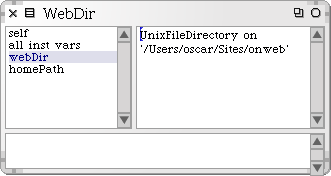
\includegraphics[width=0.8\textwidth]{aWebDir}
\caption{Une instance de WebDir.}
\figlabel{aWebDir}
\end{center}
\end{figure}

Ce serait bien de pouvoir instancier un \ct{WebDir} de façon
programmatique: ajoutons donc une autre méthode de création.

\dothis{Ajoutez les méthodes suivantes et essayez-les en inspectant le
  résultat de \mbox{\lct{WebDir onPath: '\emph{le chemin vers votre site web}'}}.}

\begin{code}{}
WebDir class>>>onPath: path home: homePath
	^ self new setDir: (FileDirectory on: path) home: homePath

WebDir class>>>onPath: homePath
	^ self onPath: homePath home: homePath
\end{code}

%-----------------------------------------------------------------
\subsection{Le \patmatch de fichiers HTML}

Pour l'instant, tout va bien.
%So far so good.
Nous aimerions utiliser maintenant les \expregs{} pour trouver quels
fichiers HTML ce site web contient.

Si nous naviguons dans la classe \ct{FileDirectory}, nous trouvons la
méthode \ct{fileNames} qui liste tous les fichiers dans un répertoire.
Nous voulons choisir uniquement ceux dont l'extension de fichier est
\ct{.html}. L'\expreg dont nous avons besoin est \ct{'.*\.html'}.
Le premier point correspond à n'importe quel caractère excepté le
retour-chariot (désignant une nouvelle ligne):
%The first dot will match any character except a newline:

% BUG HERE last should be false
\begin{code}{@TEST}
'x' matchesRegex: '.' --> true
' ' matchesRegex: '.'  --> true
Character cr asString matchesRegex: '.' --> false
\end{code}
%Character cr asString matchesRegex: '.' --> true

%\index{Regex syntax!@\ct{*}}
\index{Regex!syntaxe!@\ct{*}}
Le caractère \ct{*} (connu sous le nom de ``\ind{\kleenestar}'' ou ``étoile de Kleene'',
%``\ind{Kleene star}''
\seeindex{étoile de Kleene}{\kleenestar}
d'après Stephen Kleene, son inventeur)
définit une \expreg qui correspondra à la concordance de la
précédente \expreg zéro ou plusieurs fois.
% is a regex operator that will match the preceding regex any number of times (including zero).

\mthindex{String}{matchesRegex:}
\begin{code}{@TEST}
'' matchesRegex: 'x*'     --> true
'x' matchesRegex: 'x*'   --> true
'xx' matchesRegex: 'x*' --> true
'y' matchesRegex: 'x*'   --> false
\end{code}

\index{Regex!syntaxe!@\ct{.}}
Puisque le point est un caractère spécial dans les \expregs, 
nous devons le précéder d'un caractère d'échappement 
% ajout - vf
\lct{\symbol{92}} % backslash
si nous voulons avoir une concordance avec un vrai point dans la
chaîne de caractères.
%if we want to literally match a dot, then we must escape it.

\begin{code}{@TEST}
'.' matchesRegex: '.'   --> true
'x' matchesRegex: '.'  --> true
'.' matchesRegex: '\.'  --> true
'x' matchesRegex: '\.' --> false
\end{code}

Vérifiez maintenant que notre \expreg fonctionne pour trouver des fichiers
HTML.

\begin{code}{@TEST}
'index.html' matchesRegex: '.*\.html' --> true
'foo.html' matchesRegex: '.*\.html'    --> true
'style.css' matchesRegex: '.*\.html'   --> false
'index.htm' matchesRegex: '.*\.html' --> false
\end{code}

Cela semble bon! Nous pouvons l'essayer désormais dans notre application. 
%Looks good. Now let's try it out in our application.

\dothis{Ajoutez la méthode suivante à la classe \ct{WebDir} et
  essayez-la dans votre site web de test.}

\begin{code}{}
WebDir>>>htmlFiles
	^ webDir fileNames select: [ :each | each matchesRegex: '.*\.html' ]
\end{code}

Si vous envoyez le message \ct{htmlFiles} à une instance de
\ct{WebDir} et que vous l'imprimez via \menu{print it}, vous devriez
voir quelque chose de la sorte:

\begin{code}{}
(WebDir onPath: '...') htmlFiles --> #('index.html' ...)
\end{code}

%-----------------------------------------------------------------
\subsection{Mettre en cache l'\expreg}
%\subsection{Caching the regex}

Si vous naviguez dans la méthode \mthind{String}{matchesRegex:}, vous
découvrirez que c'est une extension de méthode de \ct{String}
qui crée une nouvelle instance de \clsind{RxParser} à chaque envoi.
C'est correct pour des requêtes \emph{ad hoc} mais si nous appliquons
la même \expreg pour chaque fichier du site web, créer une unique
instance de \ct{RxParser} pour la réutiliser est plus judicieux.
C'est ce que nous allons faire.
% you will discover that it is an extension method of \ct{String} that creates a fresh instance of \clsind{RxParser} every time it is sent.  That is fine for ad hoc queries, but if we are applying the same regex to every file in a web site, it is smarter to create just one instance of \ct{RxParser} and reuse it. Let's do that.

\dothis{Ajoutez à la classe \ct{WebDir} une nouvelle variable
  d'instance \ct{htmlRegex} et initialisez-la en envoyant le message
  \ct{asRegex} à notre chaîne de caractères d'\expreg.
Modifiez la méthode \ct{WebDir>>>htmlFiles} pour utiliser la même
\expreg tout le temps:}

\begin{code}{}
WebDir>>>initialize
	htmlRegex := '.*\.html' asRegex

WebDir>>>htmlFiles
	^ webDir fileNames select: [ :each | htmlRegex matches: each ]
\end{code}

Lister les fichiers HTML devrait fonctionner comme avant, à
l'exception de l'objet \emph{regex} que nous réutiliserons plusieurs
fois.

%-----------------------------------------------------------------
\subsection{Accéder aux pages web}

Accéder aux détails d'une page web seule devrait être la
responsabilité d'une classe distincte; définissons-la et faisons en
sorte que la classe \ct{WebDir} crée des instances de cette classe.

\dothis{Définissez une classe \ct{WebPage} avec les variables
  d'instance \ct{path} et \ct{homePath} pour identifier le fichier
  HTML et le répertoire racine du site respectivement (nous aurons
  besoin de générer les liens depuis le répertoire racine du site web jusqu'aux
  fichiers qu'il contient). Définissez une méthode d'initialisation
  côté instance et une méthode de création côté classe.}

% IMPORTANT: martial - dans la VO c'est #initializePath:homePath: , je
% préfère mettre comme dans le code source #setPath:homePath:
\begin{code}{}
WebPage>>>setPath: filePath homePath: dirPath 
	path := filePath.
	homePath := dirPath

WebPage class>>>on: filePath forHome: homePath
	^ self new setPath: filePath homePath: homePath
\end{code}

Une instance de \ct{WebDir} devrait être capable de retourner une
liste de toutes les pages web qu'elle contient.

\dothis{Ajoutez la méthode suivante à \ct{WebDir} et inspectez la
  valeur de retour pour vérifier que ça fonctionne.}

\begin{code}{}
WebDir>>>webPages
	^ self htmlFiles collect: 
		[ :each | WebPage 
			on: webDir pathName, '/', each
			forHome: homePath ]
\end{code}

\noindent{} Vous pouvez voir de la forme suivante:

\begin{code}{}
(WebDir onPath: '...') webPages --> an Array(a WebPage a WebPage ...)
\end{code}

%-----------------------------------------------------------------
\subsection{Substitutions de chaînes de caractères}
%String substitutions

Le précédent résultat ne nous informe pas beaucoup; utilisons une
\expreg pour récupérer le nom de fichier de chaque page web.
Pour ce faire, nous voulons extraire tous les caractères du chemin (ou
\emph{path name}) jusqu'au dernier répertoire. Sur le système de
fichiers Unix, les répertoires finissent par un \emph{slash} (\ct{/}),
donc nous avons besoin d'éliminer tout jusqu'au dernier \emph{slash}
dans le chemin.

La méthode d'extension de \ct{String}
\mthind{String}{copyWithRegex:matchesReplacedWith:} fait cela pour
nous:

\begin{code}{@TEST}
'hello' copyWithRegex: '[elo]+' matchesReplacedWith: 'i' --> 'hi'
\end{code}

\index{Regex!syntaxe!@\ct{+}}
Dans cet exemple, l'\expreg \ct{[elo]} correspond à un caractère
pouvant être \ct{e}, \ct{l} ou \ct{o}. % CHANGE : ajout - vf : "à un"
                                % plutôt que "n'importe qu'"
% matches any of the characters \ct{e}, \ct{l} or \ct{o}.
L'opérateur \ct{+} est comme la \kleenestar, mis à part qu'il
correspond exactement à \emph{une} ou plusieurs instances de l'\expreg
qui le précède. Il correspondra ici à la sous-chaîne \ct{'elo'} qui
sera remplacée par la lettre \ct{i} pour générer une nouvelle chaîne de
caractères.
\index{Regex!syntaxe!@\ct{+}}

\dothis{Ajoutez la méthode suivante et vérifiez qu'elle fonctionne
  comme attendu.}

\begin{code}{}
WebPage>>>fileName
	^ path copyWithRegex: '.*/' matchesReplacedWith: ''
\end{code}

\noindent{} Vous devriez voir quelque chose comme ça sur votre site de test: 

\begin{code}{}
(WebDir onPath: '...') webPages collect: [:each | each fileName ]
  --> #('index.html' ...)
\end{code}

%-----------------------------------------------------------------
\subsection{Extraire les \regexmatches}
%extracting regex matches

L'étape suivante est l'extraction de titre de chaque page HTML.

Tout d'abord, nous avons besoin de trouver une façon de récupérer le
contenu de chaque page. Vous allez voir que c'est simple.

\dothis{Ajoutez la méthode suivante et essayez-la.}

\mthindex{FileStream}{oldFileOrNoneNamed:}
\begin{code}{}
WebPage>>>contents
	^ (FileStream oldFileOrNoneNamed: path) contents
\end{code}

En fait, vous pourriez avoir des problèmes si vos pages web
contiennent des caractères non-ascii. Dans ce cas, il serait plus sûr
d'écrire la méthode ainsi:

\clsindex{Latin1TextConverter}
\begin{code}{}
WebPage>>>contents
	^ (FileStream oldFileOrNoneNamed: path)
		converter: Latin1TextConverter new;
		contents
\end{code}

\noindent{} Vous devriez maintenant pouvoir voir quelque chose semblable à ceci:

\begin{code}{}
(WebDir onPath: '...') webPages first contents --> '<head>
<title>Titre de la !\normcode{première}! page</title>
...
'
\end{code}

Passons à l'extraction du titre. Dans ce cas, nous chercherons le
texte situé \emph{entre} les balises HTML \ct{<title>} et \ct{</title>}. 

\index{Regex!syntaxe!@\ct{^}}
Nous avons besoin de trouver une manière d'extraire la \emph{partie}
d'une concordance dit aussi \ind{\regexmatch} d'une \expreg. Les
sous-expressions des \expregs sont délimitées par des parenthèses.
Considérons l'\expreg \ct{([CARETaeiou]+)([aeiou]+)}. 
Elle comprend deux sous-expressions; la première correspondera à une
séquence d'un ou plusieurs caractères qui n'est pas une voyelle et la
seconde correspondera à une ou plusieurs voyelles. \arelire{L'opérateur
\ct{CARET} au début de l'ensemble de caractères entre crochets
contredit cet ensemble \cad qu'il le transforme en l'ensemble
complémentaire~\footnote{NB: Dans \pharo,
  l'accent circonflexe (appelé aussi \emph{caret}) correspond aussi au
  mot-clé de \emph{retour} que nous écrivons \ct{^}. Pour éviter toute
  confusion, nous écrirons \ct{CARET} lorsque nous utiliserons
  l'accent circonflexe dans les expressions régulières pour les
  ensembles complémentaires mais vous devez vous souvenir que ces
  symboles sont en réalité les mêmes.}.}
  %  To avoid
  % confusion, we will write \ct{CARET} when we are using the caret
  % within regular expressions to negate sets of characters, but you
  % should not forget, they are actually the same thing.}}.

\arelire{Nous allons désormais essayer de faire correspondre l'\expreg
  à un \emph{préfixe}~\footnote{En anglais, \emph{prefix}.} de la chaîne de
caractères \ct{'pharo'} et extraire les sous-éléments de cette concordance:}
% Now we will try to match a \emph{prefix} of the string \ct{'pharo'}
% and extract the submatches:

\mthindex{RxMatcher}{matchesPrefix:}
\mthindex{RxMatcher}{subexpression:}
\begin{code}{| re |}
re := '([CARETaeiou]+)([aeiou]+)' asRegex.
re matchesPrefix: 'pharo' --> true
re subexpression: 1         --> 'pha'
re subexpression: 2         --> 'ph'
re subexpression: 3         --> 'a'
\end{code}

Après la concordance réussie entre une \expreg et une chaîne de
caractères, \arelire{vous pouvez toujours envoyer à cette concordance
  ou \emph{match} le message} \ct{subexpression: 1} pour extraire la
concordance entière.
Vous pouvez aussi envoyer \lct{subexpression: $n$} où $n-1$ est le
nombre de sous-expressions dans l'\expreg. L'\expreg ci-dessus a deux
sous-expressions, numérotées $2$ et $3$.

Nous utiliserons la même astuce pour extraire le titre dans un fichier
HTML.

\dothis{Définissez la méthode suivante:}

\mthindex{String}{asRegexIgnoringCase}
\begin{code}{}
WebPage>>>title
	| re |
	re := '[\w\W]*<title>(.*)</title>' asRegexIgnoringCase.
	^ (re matchesPrefix: self contents)
		ifTrue: [ re subexpression: 2 ]
		ifFalse: [ '(', self fileName, ' -- sans titre)' ]
\end{code} % ajout vf - remplacement de 'untitled'
% \begin{code}{}
% WebPage>>>title
% 	| re |
% 	re := '[\w\W]*<title>(.*)</title>' asRegexIgnoringCase.
% 	^ (re matchesPrefix: self contents)
% 		ifTrue: [ re subexpression: 2 ]
% 		ifFalse: [ '(', self fileName, ' -- untitled)' ]
% \end{code}

Deux cas subtils sont à prendre en compte ici.
Premièrement, le code HTML ne s'intéresse pas à savoir si les balises
sont en minuscule ou en majuscule donc nous devons faire en sorte que
notre \expreg soit insensible à la casse en l'instanciant avec le
message \mbox{\ct{asRegexIgnoringCase}.}

Deuxièmement, puisque le point correspond à n'importe quel caractère \arelire{%
\emph{à l'exception des retours-chariot}}, l'\expreg 
%\emph{except a newline}
\mbox{\lct{.*<title>(.*)</title>}} ne fonctionnera comme prévu que si
plusieurs lignes apparaissent avant le titre.
L'\expreg \ct{\w} correspond à \arevoir{n'importe quel caractère alpha-numérique} 
%matches any alphanumeric,
et \ct{\W} correspond à \arevoir{n'importe quel caractère non
  alpha-numérique}; \ct{[\w\W]} correspond donc à \arevoir{n'importe
  quel caractère \emph{incluant le retour-chariot}} (Si nous nous
  attendons à ce que les titres contiennent des
  \arelire{retours-chariot}, nous devrons utiliser la même technique
  dans la sous-expression).

Nous pouvons tester maintenant notre extracteur de titre et nous
devrions obtenir quelque chose comme ça:

\begin{code}{}
(WebDir onPath: '...') webPages first title --> 'Pharo By Example -- Home Page'
\end{code}
% \begin{code}{}
% (WebDir onPath: '...') webPages first title --> 'Home page'
% \end{code}

%-----------------------------------------------------------------
\subsection{Plus de substitutions de chaînes de caractères}
%\subsection{More string substitutions}

Pour générer notre \sitemap, nous aurons besoin de générer les liens
vers chaque page.
Nous pouvons utiliser le titre de la page comme nom de lien. Nous
aurons besoin simplement de générer le chemin correct vers la page web
depuis la racine du site web.
Par chance, c'est trivial\,---\,c'est tout simplement le chemin
complet de la page web moins le chemin complet vers le répertoire
racine du site web.

Nous devons tout de même faire attention à une chose. Comme la
variable \ct{homePath} ne se termine pas par un \ct{/}, nous devrons
veiller à l'ajouter, sinon le chemin relatif des liens commencera par
un \ct{/}.
Notez la différence entre les deux résultats suivants:

\mthindex{String}{copyWithRegex:matchesReplacedWith:}
\begin{code}{}
'/home/testweb/index.html' copyWithRegex: '/home/testweb' matchesReplacedWith: '' --> '/index.html'
'/home/testweb/index.html' copyWithRegex: '/home/testweb/' matchesReplacedWith: '' -->  'index.html'
\end{code}

Le premier résultat nous donne un chemin absolu; ce n'est pas ce que
nous voulons.

\dothis{Définissez les méthodes suivantes:}

\begin{code}{}
WebPage>>>relativePath
	^ path 
		copyWithRegex: homePath , '/'
		matchesReplacedWith: ''

WebPage>>>link
	^ '<a href="', self relativePath, '">', self title, '</a>'
\end{code}

Testez donc le code suivant pour voir votre premier lien:
% CHANGE - vf - martial : trop de 'you should now be able ...' 
%You should now be able to see something like this:

% \begin{code}{}
% (WebDir onPath: '...') webPages first link --> '<a href="index.html">Home Page</a>'
% \end{code}
\begin{code}{}
(WebDir onPath: '...') webPages first link --> '<a href="index.html">Pharo By Example -- Home Page</a>'
\end{code}

%-----------------------------------------------------------------
\subsection{Générer le \sitemap}

Voilà! Nous en avons fini avec les \expregs pour ce qui concerne notre
exemple de générateur de \sitemap.
% Actually, we are now done with the regular expressions we need to
% generate the site map.
Nous aurons besoin de quelques méthodes pour compléter l'application.

\dothis{Si vous voulez voir la génération du \sitemap, ajoutez
  simplement les méthodes suivantes.}

Si votre site web contient des sous-répertoires, nous avons besoin
d'une méthode pour y accéder:
\begin{code}{}
WebDir>>>webDirs
	^ webDir directoryNames
		collect: [ :each | WebDir onPath: webDir pathName , '/' , each home: homePath ]
\end{code}

Nous avons besoin aussi de générer la liste à puces contenant les
liens vers chaque page web d'un répertoire web.
\arevoir{Les sous-répertoires devraient être indentés dans leur propre liste à puces.}
% Subdirectories should be indented in their own bullet list.
\begin{code}{}
WebDir>>>printTocOn: aStream 
	self htmlFiles
		ifNotEmpty: [
			aStream nextPutAll: '<ul>'; cr.
			self webPages
				do: [:each | aStream nextPutAll: '<li>';
						 nextPutAll: each link;
						 nextPutAll: '</li>'; cr].
			self webDirs
				do: [:each | each printTocOn: aStream].
			aStream nextPutAll: '</ul>'; cr]
\end{code}

Nous créons un fichier appelé ``toc.html''\footnote{\arelire{NdT: ``toc'' est
  l'abrégé de \emph{Table Of Contents} \cad ``table des matières''.}}
dans le répertoire racine du site web et nous y déposerons notre
\sitemap.
% We create a file called ``toc.html'' in the root web directory and dump the site map there.
\begin{code}{}
WebDir>>>tocFileName
	^ 'toc.html'

WebDir>>>makeToc
	| tocStream |
	tocStream := webDir newFileNamed: self tocFileName.
	self printTocOn: tocStream.
	tocStream close.
\end{code}

Générons maintenant une table des matières pour un répertoire web de
votre choix!
\begin{code}{}
WebDir selectHome makeToc
\end{code}

\begin{figure}[tbh]
\begin{center}
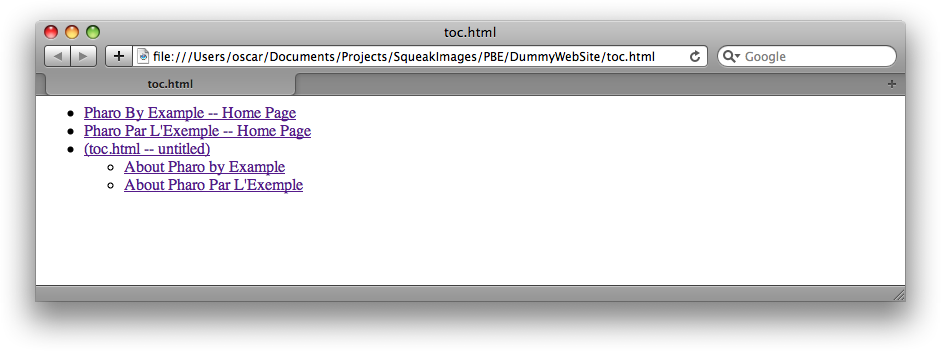
\includegraphics[width=\textwidth]{PBE-toc}
\caption{Un mini-\sitemap.}
\figlabel{PBE-toc}
\end{center}
\end{figure}

%=================================================================
\section{La syntaxe des \expregs}
\index{expression!syntaxe des \expregs}
%\section{Regex syntax}\indexmain{Regex syntax}

Nous allons voir plus en détail la syntaxe des \expreg telle qu'elle
est supportée par le paquetage \pkgregex.

L'\expreg la plus simple est un caractère unique. Elle correspond
exactement à ce caractère. Une séquence de caractères correspond à une
chaîne de caractères ayant exactement la même séquence de caractères:
\mthindex{String}{matchesRegex:}
\begin{code}{@TEST}
'a' matchesRegex: 'a'                  --> true
'foobar' matchesRegex: 'foobar'  --> true
'blorple' matchesRegex: 'foobar' --> false
\end{code}

Les opérateurs sont appliqués aux \expregs pour produire des \expregs
plus complexes.
\aretirer{Le séquençage (\cad l'ordonnancement des expressions les unes à la
  suite des autres) est, en un sens, ``invisible'' en ce qui concerne
  les opérateurs\,---\,quoique c'est le plus commun.} % REVOIR CHANGE
%  Sequencing (placing expressions one
% after another) as an operator is, in a certain sense,
% ``invisible''\,---\,yet it is arguably the most common.

\indexmain{Regex!syntaxe!@\ct{*}}
Nous avons déjà vu la \ind{\kleenestar} (\ct{*}) et l'opérateur \ct{+}.
Une \expreg suivie par une \kleenestar correspond à un certain nombre
(incluant $0$) de concordances de l'expression originale. Par exemple:
\begin{code}{@TEST}
'ab' matchesRegex: 'a*b'         --> true
'aaaaab' matchesRegex: 'a*b' --> true
'b' matchesRegex: 'a*b'           --> true
'aac' matchesRegex: 'a*b'	    --> false    "b ne correspond pas"
\end{code}

\index{Regex!priorité des opérateurs}
%\index{Regex!operator precedence}
La \kleenestar a une plus grand priorité que le séquençage. Une
\kleenestar s'applique à la sous-expression la plus 
\arevoir{courte possible qui la précède}.
%shortest possible subexpression that precedes it.
Par exemple, \ct{ab*} signifie \ct{a} suivi par zéro ou plusieurs
occurences de \ct{b} et non, ``zéro ou plusieurs fois \ct{ab}'':
occurrences of \ct{ab}'':
\begin{code}{@TEST}
'abbb' matchesRegex: 'ab*' --> true
'abab' matchesRegex: 'ab*' --> false
\end{code}

\indexmain{Regex!syntaxe!@\ct{()}}
Pour obtenir une \expreg qui correspond à ``zéro ou plusieurs
occurrences de \ct{ab}'', nous devons inclure \ct{ab} entre
parenthèses:
\begin{code}{@TEST}
'abab' matchesRegex: '(ab)*'   --> true
'abcab' matchesRegex: '(ab)*' --> false    "c joue les !trouble-fête!"
\end{code} % vf - note: trouble-fête au pluriel, c'est exact!

\indexmain{Regex!syntaxe!@\ct{+}}
\indexmain{Regex!syntaxe!@\ct{?}}
Deux autres opérateurs bien utiles, semblables à \ct{*}, sont \ct{+}
et \ct{?}. \ct{+} correspond à une ou plusieurs instances de l'\expreg
qu'il modifie. \ct{?} assurera la concordance avec zéro ou une
instance.
% ajout - vf - CHANGE
Ces trois opérateurs sont appelés des \emph{quantificateurs}.
\begin{code}{@TEST}
'ac' matchesRegex: 'ab*c'	   --> true
'ac' matchesRegex: 'ab+c'	  --> false    "besoin d'au moins un b"
'abbc' matchesRegex: 'ab+c' --> true
'abbc' matchesRegex: 'ab?c' --> false    "trop de b"
\end{code}

\indexmain{Regex!syntaxe!\escchar}
Comme nous l'avons vu, les caractères \ct{*}, \ct{+}, \ct{?}, \ct{(},
et \ct{)} ont un sens spécial dans les \expregs. Si nous avons besoin
de faire correspondre n'importe lequel d'entre eux de manière
littérale, il faudrait l'\emph{échapper} en précédant ce caractère par
un \escchar \cad un \mbox{\emph{antislash} (\lct{\symbol{92}}).} L'\emph{antislash} est
  aussi un caractère spécial et a donc besoin d'être précédé par
  \escchar pour qu'il y ait concordance. Ceci est aussi valable pour
  tous les caractères spéciaux que nous pourrions voir plus loin.
\begin{code}{@TEST}
'ab*' matchesRegex: 'ab*'  --> false    "l'!astérisque! est !spécial!"
'ab*' matchesRegex: 'ab\*' --> true
'a\c' matchesRegex: 'a\\c'  --> true
\end{code}

\indexmain{Regex!syntaxe!@\ct{|}}
Le dernier opérateur est \ct{|}; il exprime un choix entre deux
sous-expressions. Il correspond à une chaîne de caractères si l'une des
deux expressions concorde. Cet opérateur à la priorité la plus
basse\,---\,inférieure même au séquençage.
%It has the lowest precedence\,---\,even lower than sequencing.
Par exemple, \ct{ab*|ba*} signifie ``a suivi par un certain nombre de
b \emph{ou} b suivi par un certain nombre de a'':
\begin{code}{@TEST}
'abb' matchesRegex: 'ab*|ba*'   --> true
'baa' matchesRegex: 'ab*|ba*'	--> true
'baab' matchesRegex: 'ab*|ba*' --> false
\end{code}

Voici un exemple un peu plus compliqué. L'expression \ct{c(a|d)+r}
correspond au nom de n'importe quelle fonction
historique\footnote{NdT: voir \url{http://fr.wikipedia.org/wiki/Lisp}} du langage de programmation Lisp: 
 \ct{car}, \ct{cdr}, \ct{caar}, \ct{cadr}\ldots:
\begin{code}{@TEST}
'car' matchesRegex: 'c(a|d)+r'   --> true
'cdr' matchesRegex: 'c(a|d)+r'   --> true
'cadr' matchesRegex: 'c(a|d)+r' --> true
\end{code} % CHANGE - martial - note de bas de page sur Lisp

Il est possible d'écrire une expression qui correspond à une chaîne
vide; par exemple, l'\expreg \ct{a|} correspond à une chaîne vide.
Cependant, appliquer  \ct{*}, \ct{+} ou \ct{?} tel quel est une
erreur: \ct{(a|)*}, en revanche, est valide.

%\indexmain{Regex!syntaxe!character set}
\indexmain{Regex!syntaxe!classe de caractères}
Nous n'avons utilisé que des caractères comme \emph{plus petits}
composants des \expregs.
% So far, we have used only characters as the \emph{smallest}
% components of regular expressions.
Il y a d'autres composants plus intéressants encore. Une \emph{classe
de caractères} est une chaîne de caractères entre crochets: il
correspond à un simple caractère s'il apparaît entre les crochets. Par
exemple, \ct{[01]} correspond à \ct{0} ou \ct{1}:
\begin{code}{@TEST}
'0' matchesRegex: '[01]'   --> true
'3' matchesRegex: '[01]'   --> false
'11' matchesRegex: '[01]' --> false  "une classe correspond !à! un !caractère! seulement"
\end{code}

En utilisant l'opérateur \ct{+}, nous pouvons construire un outil de
reconnaissance de nombre binaire:
\begin{code}{@TEST}
'10010100' matchesRegex: '[01]+' --> true
'10001210' matchesRegex: '[01]+' --> false
\end{code}

Si le premier caractère après le crochet ouvrant est \ct{CARET},
la classe de caractères est inversée: la concordance se fait donc sur
un caractère qui \emph{n'est pas} entre les crochets:
% the set is inverted: it matches any single character \emph{not} appearing between the brackets:
\begin{code}{@TEST}
'0' matchesRegex: '[CARET01]' --> false
'3' matchesRegex: '[CARET01]' --> true
\end{code}

%\indexmain{Regex!syntaxe!character range}
\indexmain{Regex!syntaxe!intervalle de classe}
Pour des raisons de commodité, une classe de caractères peut inclure
des intervalles: deux caractères séparés par un tiret (\ct{-})
% separated by a hyphen (\ct{-}).
forment ce que nous appelons un intervalle de classe.
Cet intervalle est équivalent à la liste complète de tous les
caractères entre ces deux caractères:  \ct{'[0-9]'} est la même chose
que  \ct{'[0123456789]'}.
Les caractères spéciaux dans une classe de caractères sont 
\ct{CARET}, \ct{-}, et \ct{]}; ce dernier clôt la classe. 
Ci-dessous, nous avons \arelire{des exemples montrant comment les
  utiliser dans une classe pour en faire la concordance}:
% which closes the set. Below are examples how to literally match them
% in a set:
\begin{code}{@TEST}
'CARET' matchesRegex: '[01CARET]'   --> true    "mettre l'accent partout sauf au !début!"
'-' matchesRegex: '[01-]' --> true    "mettre le tiret !à! la fin"
']' matchesRegex: '[]01]'   --> true    "mettre le crochet fermant au !début!"
\end{code}

\noindent{} \arevoir{Les classes vides et universelles ne peuvent pas être
  définies.}
% Thus, empty and universal sets cannot be specified.

%-----------------------------------------------------------------
\subsection{Les classes de caractères abrégées}
%\subsection{Character classes}
Les \expregs{} peuvent aussi inclure les échappements avec
\emph{antislash} suivants appelés ``classes de caractères abrégées'':
\ct{\w} correspondant aux caractères alphanumériques (``w'' pour
\emph{word}), \ct{\d} correspondant aux chiffres (``d'' pour
\emph{digit}) et \ct{\s} correspondant à l'espace (``s'' pour
\emph{space}).
Les variantes majuscules, \ct{\W}, \ct{\D} et \ct{\S}, correspondent
aux caractères complémentaires (respectivement pour les caractères
non-alphanumeriques, les non-chiffres et tous les caractères qui ne
sont pas un espace).
Nous pouvons voir un résumé de la syntaxe \pkgregex dans
\tabref{regexsyntax}.

\indexmain{Regex!syntaxe}
\begin{table}
\centering
	\begin{tabular}{lp{8cm}}
		\toprule
		Syntaxe \pkgregex & Représentation \\
		\midrule
		\lct{a}				&	concorde avec le caractère \lct{a} \\
		\lct{.}				&	concorde avec n'importe quel caractère (sauf retour-chariot) \\
		\lct{($\cdots$)}		&	\arevoir{sous-expression groupée} \\ %group subexpression \\
		\lct{{\escape}}	&	caractère d'échappement \\ %escape following special character \\
		\midrule
		\lct{*}				&	\kleenestar\,---\,concorde avec zéro ou plusieurs \expregs précédentes \\
		\lct{+}				&	concorde avec une ou plusieurs \expregs précédentes \\
		\lct{?}				&	concorde avec zéro ou une \expreg précédente \\
		\lct{|}				&	concorde avec l'\expreg de droite ou de gauche \\
		\midrule
		\lct{[abcd]}		&	concorde avec un caractère de la liste \lct{abcd} \\ %match choice of characters \lct{abcd} \\
		\lct{[{\caret}abcd]}	&	concorde avec un caractère de la liste complémentaire \\%match negated choice of characters \\
		\lct{[0-9]}		&	concorde avec un caractère dans l'intervalle compris entre \lct{0} et \lct{9} \\
		\midrule
		\lct{{\escape}w}			&	concorde avec un caractère alphanumérique \\
		\lct{{\escape}W}			&	concorde avec un caractère non-alphanumérique \\
		\lct{{\escape}d}			&	concorde avec un chiffre \\
		\lct{{\escape}D}			&	concorde avec un non-chiffre \\
		\lct{{\escape}s}			&	concorde avec l'espace \\
		\lct{{\escape}S}			&	concorde avec un caractère qui n'est pas un espace \\
		\bottomrule
	\end{tabular}
	\caption{Résumé de la syntaxe \pkgregex{.}\tablabel{regexsyntax}}
\end{table}


Comme nous l'avons dit dans l'introduction, les \expregs sont surtout
utiles pour valider les saisies de l'utilisateur et les classes
abrégées sont particulièrement utiles pour définir de telles \expregs.
Par exemple, les nombres non-négatifs peuvent être filtrés avec
l'\expreg \ct{\d+}:

\begin{code}{@TEST}
'42' matchesRegex: '\d+' --> true
'-1' matchesRegex: '\d+' --> false
\end{code}

Nous pouvons encore vouloir préciser que les nombres non-négatifs ne
doivent pas commencer par le chiffre 0:
\tradalert{martial}{Better yet, we might want to specify that
  \textbf{non-zero numbers}}

\needlines{4}
\begin{code}{@TEST}
'0' matchesRegex: '0|([1-9]\d*)'     --> true
'1' matchesRegex: '0|([1-9]\d*)'     --> true
'42' matchesRegex: '0|([1-9]\d*)'   --> true
'099' matchesRegex: '0|([1-9]\d*)' --> false    "!débute! par !zéro!"
\end{code}

\noindent{} Nous pouvons vérifier l'expression avec des nombres négatifs et positifs:

\begin{code}{@TEST}
'0' matchesRegex: '(0|((\+|-)?[1-9]\d*))'     --> true
'-1' matchesRegex: '(0|((\+|-)?[1-9]\d*))'   --> true
'42' matchesRegex: '(0|((\+|-)?[1-9]\d*))'   --> true
'+99' matchesRegex: '(0|((\+|-)?[1-9]\d*))' --> true
'-0' matchesRegex: '(0|((\+|-)?[1-9]\d*))'   --> false    "!zéro! !négatif!"
'01' matchesRegex: '(0|((\+|-)?[1-9]\d*))'   --> false    "!débute! par !zéro!"
\end{code}

Les nombres à virgule flottante exigeraient au moins un chiffre après
le point\footnote{NdT: le point remplace la virgule dans la convention
  informatique de la notation informatique.}: 

\begin{code}{@TEST}
'0' matchesRegex: '(0|((\+|-)?[1-9]\d*))(\.\d+)?'      --> true
'0.9' matchesRegex: '(0|((\+|-)?[1-9]\d*))(\.\d+)?'   --> true
'3.14' matchesRegex: '(0|((\+|-)?[1-9]\d*))(\.\d+)?' --> true
'-42' matchesRegex: '(0|((\+|-)?[1-9]\d*))(\.\d+)?'  --> true
'2.' matchesRegex: '(0|((\+|-)?[1-9]\d*))(\.\d+)?'     --> false "manque des chiffres !après! ."
\end{code}

%Checking if aString is a fixed-point number, with at least one digit is required after a dot:
%\begin{code}{}
%'' matchesRegex: '(\+|-)?\d+(\.\d+)?'
%The same, but allow notation like '123.':
%'' matchesRegex: '(\+|-)?\d+(\.\d*)?'
%\end{code}
%Recognizer for a string that might be a name: one word with first capital letter, no blanks, no digits.  More traditional:
%\begin{code}{}
%'' matchesRegex: '[A-Z][A-Za-z]*'
%more Smalltalkish:
%'' matchesRegex: ':isUppercase::isAlphabetic:*'
%\end{code}
%A date in format MMM DD, YYYY with any number of spaces in between, in XX century:
%\begin{code}{}
%'' matchesRegex: '(Jan|Feb|Mar|Apr|May|Jun|Jul|Aug|Sep|Oct|Nov|Dec)[ ]+(\d\d?)[ ]*,[ ]*19(\d\d)'
%\end{code}
%Note parentheses around some components of the expression above. As the Usage Section shows, they will allow us to obtain the actual strings that have matched them (\ie month name, day number, and year number).

En bonus, voici un filtre pour un format générique de nombres, valable
pour des nombres comme \ct{999}, or \ct{999.999} ou \ct{-999.999e+21}.
\begin{code}{@TEST}
'-999.999e+21' matchesRegex: '(\+|-)?\d+(\.\d*)?((e|E)(\+|-)?\d+)?' --> true
\end{code}

Les classes abrégées peuvent aussi inclure les éléments compatibles
\ct{grep(1)} listés dans \tabref{charclasses}.
%Character classes can also include the grep(1)-compatible elements listed in \tabref{charclasses}.

\indexmain{Regex!syntaxe!classe de caractère abrégée}
\begin{table}[htb]
\centering
	\begin{tabular}{lp{8cm}}
		\toprule
	Syntaxe \pkgregex & Représentation \\
		\midrule
\lct{[:alnum:]} & alphanumérique \\
\lct{[:alpha:]} & caractère alphabétique\\
\lct{[:cntrl:]} & caractère Control (code ASCII \lct{< 32})\\
\lct{[:digit:]} & chiffre décimal\\
\lct{[:graph:]} & caractère graphique (code ASCII \lct{>= 32})\\
\lct{[:lower:]} & caractère en minuscule\\
\lct{[:print:]} & caractère imprimable (ici, le même que \lct{[:graph:]})\\
\lct{[:punct:]} & caractère de ponctuation\\
\lct{[:space:]} & caractère espace\\
\lct{[:upper:]} & caractère en majuscule\\
\lct{[:xdigit:]} & caractère hexadécimal\\
		\bottomrule
	\end{tabular}
	\caption{Les classes de caractères abrégées de \pkgregex.\tablabel{charclasses}}
\end{table}

Notez que ces éléments font partie des classes abrégées; ils doivent
être inclus dans un ensemble de crochets pour former une \expreg
valide. Par exemple, un filtrage de chaînes de caractères non-vides composées
uniquement de chiffres devrait être représenté par \ct{[[:digit:]]+}.
Les expressions et opérateurs primitifs précédemment vus sont communs
à de nombreuses implémentations d'\expregs.
% they have to be enclosed in an extra set of square brackets to form a valid regular expression.  For example, a non-empty string of digits would be represented as \ct{[[:digit:]]+}. The above primitive expressions and operators are common to many implementations of regular expressions.

\begin{code}{@TEST}
'42' matchesRegex: '[[:digit:]]+' --> true
\end{code}

%-----------------------------------------------------------------
%\subsection{Les classes de caractères spéciales}
%\subsection{Special character classes}
\subsection{Les classes spéciales}
L'expression simple suivante est unique à l'implémentation \st. Une
séquence de caractères entre \emph{deux-points} est traitée comme un
sélecteur unaire \arevoir{qui peut être compris par les caractères}.
% A sequence of characters between colons is treated as a unary
% selector which is supposed to be understood by characters
Un caractère correspond à une telle expression s'il répond \ct{true}
à un message formé par ce sélecteur.
% A character matches such an expression if it answers true to a
% message with that selector.
Ceci offre une façon plus lisible et plus efficace de spécifier les
classes de caractères. Par exemple, \ct{[0-9]} est équivalent à
\ct{:isDigit:}, mais la dernière est plus efficace. Par analogie aux
classes de caractères, les classes spéciales peuvent avoir un négatif:
\ct{:CARETisDigit:} concorde avec un caractère qui répond \ct{false} à
 \ct{isDigit} et est ainsi équivalent à  \ct{[CARET0-9]}.

Nous avons donc déjà vu les façons suivantes (toutes équivalentes) pour écrire une \expreg qui
correspond à une chaîne de caractères non-vide de chiffres:
\ct{[0-9]+}, \ct{\d+}, \ct{[\d]+}, \ct{[[:digit:]]+} et \ct{:isDigit:+}.

\begin{code}{@TEST}
'42' matchesRegex: '[0-9]+'      --> true
'42' matchesRegex: '\d+'           --> true
'42' matchesRegex: '[\d]+'         --> true
'42' matchesRegex: '[[:digit:]]+' --> true
'42' matchesRegex: ':isDigit:+'  --> true
\end{code}

%-----------------------------------------------------------------
%\subsection{Matching boundaries}
\subsection{Filtrage aux extrémités}
Le dernier groupe de primitives spéciales est visible dans
\tabref{boundaries} et est utilisé pour faire le filtrage aux
extrémités des chaînes de caractères.

\indexmain{Regex!syntaxe!filtrage aux extrémités}
\begin{table}[htb]
\centering
	\begin{tabular}{lp{8cm}}
		\toprule
        Syntaxe \pkgregex & Représentation \\
		\midrule
		\lct{\caret} & concorde avec une chaîne vide en début de ligne \\
		\lct{\$} & concorde avec une chaîne vide en fin de ligne \\
		\lct{{\escape}b} & concorde avec une chaîne vide à une extrémité du mot \\
		\lct{{\escape}B} & concorde avec une chaîne vide ailleurs qu'à une extrémité du mot \\
		\lct{{\escape}<} & concorde avec une chaîne vide en début de mot\\
		\lct{{\escape}>} & concorde avec une chaîne vide en fin de mot\\
		\bottomrule
	\end{tabular}
	\caption{Les primitives pour le filtrage aux extrémités.\tablabel{boundaries}}
\end{table}

\begin{code}{@TEST}
'hello world' matchesRegex: '.*\bw.*' --> true      "!extrémité! de mot avant w"
'hello world' matchesRegex: '.*\bo.*'  --> false    "pas !d'extrémité! avant o"
\end{code}

%=================================================================
\section{L'interface de programmation \pkgregex}

Nous nous sommes attardés jusqu'ici à la présentation de la syntaxe
des \expregs. Nous allons explorer maintenant les différents messages
compris par les chaînes de caractères et les \expregs.

%-----------------------------------------------------------------
%\subsection{Matching prefixes and ignoring case}
\subsection{Concordance des préfixes et l'ignorance de la casse}

La plupart de nos précédents exemples ont utilisé la méthode étendue
\ct{matchesRegex:} de la classe \ct{String}.
% So far most of our examples have used the \ct{String} extension method \ct{matchesRegex:}.

Les chaînes de caractères comprennent aussi les messages suivants:
\mthind{String}{prefixMatchesRegex:}, \mthind{String}{matchesRegexIgnoringCase:} et
\mbox{\mthind{String}{prefixMatchesRegexIgnoringCase:}.}

Le message \mthind{String}{prefixMatchesRegex:} se présente comme
\mthind{String}{matchesRegex} à l'exception que le \arelire{receveur complet}
n'est pas nécessaire pour faire la concordance avec l'\expreg passée
en argument; la concordance d'un préfixe du receveur est suffisant.
% , except that the whole receiver is not expected to match the regular expression passed as the argument; matching just a prefix of it is enough.
\begin{code}{@TEST}
'abacus' matchesRegex: '(a|b)+'                                --> false
'abacus' prefixMatchesRegex: '(a|b)+'                       --> true
'ABBA' matchesRegexIgnoringCase: '(a|b)+'            --> true
'Abacus' matchesRegexIgnoringCase: '(a|b)+'          --> false
'Abacus' prefixMatchesRegexIgnoringCase: '(a|b)+' --> true
\end{code}

% ajout vf - martial
\tradalert{martial}{j'ai complété d'un paragraphe pour le cas
  ignoringcase}
Les messages de la forme \ct{*IgnoringCase} (en français,
  ``ignorer la casse'') sont équivalents aux messages sans le suffixe
  à l'exception que les premiers ne respectent pas la casse (majuscule
ou minuscule).

%-----------------------------------------------------------------
%\subsection{Enumeration interface}
\subsection{Protocole d'énumération}

Certaines applications ont besoin d'accéder à \emph{toutes} les
concordances d'une certaine \expreg avec une chaîne de caractères.
Les concordances sont accessibles via un protocole inspiré par le
protocole d'énumeration 
% ajout vf
\prot{enumerating}
familier dans les classes des paquetages de la forme \pkg{Collection-*}.
% the familiar \ct{Collection}-like enumeration protocol.

\mthind{String}{regex:matchesDo:} évalue un bloc à un argument pour
chaque concordance d'une \expreg avec la chaîne-receveur.

\begin{code}{@TEST | list |}
list := OrderedCollection new.
'Pierre voit Pauline' regex: '\w+' matchesDo: [:word | list add: word].
list --> an OrderedCollection('Pierre' 'voit' 'Pauline')
\end{code}

\mthind{String}{regex:matchesCollect:} évalue un bloc à un argument
pour chaque concordance avec l'\expreg avec la chaîne-receveur. Il
collecte ensuite les résultats et les retourne sous la forme d'une
 \clsind{SequenceableCollection}.

\begin{code}{@TEST}
'Pierre voit Pauline' regex: '\w+' matchesCollect: [:word | word size]                          --> an OrderedCollection(6 4 7)
\end{code}

\mthind{String}{allRegexMatches:} renvoie une collection de toutes les
concordances (avec les sous-chaînes de la chaîne-receveur) de l'\expreg.

\begin{code}{@TEST}
'Pierre voit Pauline en hauteur' allRegexMatches: '\w+' --> an OrderedCollection('Pierre' 'voit' 'Pauline' 'en' 'hauteur')
\end{code}

%-----------------------------------------------------------------
\subsection{Remplacement et traduction}
% translation

Il est possible de remplacer toutes les concordances d'une \expreg
avec une certaine chaîne de caractères en utilisant le message  \mthind{String}{copyWithRegex:matchesReplacedWith:}.

\begin{code}{@TEST}
'Pierre hait Jean' copyWithRegex: '\<[[:lower:]]+\>' matchesReplacedWith: 'aime' -->  'Pierre aime Jean'
\end{code}

Une forme plus générale de substitution est la traduction de
concordance (ou \emph{match translation}). Le message suivant évalue
un bloc en lui passant chaque concordance de l'\expreg dans la
chaîne-receveur et retourne une copie du receveur avec les résultats
du bloc collé entre eux à la place des concordances respectives.
% A more general substitution is match translation. This message evaluates a block passing it each match of the regular expression in the receiver string and answers a copy of the receiver with the block results spliced into it in place of the respective matches.

\begin{code}{@TEST}
'Pierre aime Jean' copyWithRegex: '\b[a-z]+\b' matchesTranslatedUsing: [:each | each asUppercase] --> 'Pierre AIME Jean'
\end{code}

Tous les messages des protocoles d'énumération et de remplacement font
leur concordance en respectant la casse. Les versions insensibles à la
casse ne font pas partie d'un protocole de \ct{String}.
Ils sont accessibles cependant en utilisant l'interface bas niveau
présentée dans la section suivante.
%-----------------------------------------------------------------
%\subsection{Lower-level interface}
\subsection{Interface bas niveau}

Lorsque vous envoyez le message \mthind{String}{matchesRegex:} à une
chaîne de caractères, les étapes suivantes se produisent:

\begin{enumerate}
\item une nouvelle instance de \clsind{RxParser} est créée et la
  chaîne de caractères de l'\expreg lui est passée, donnant un arbre
  de syntaxe de l'expression;
\item  l'arbre de syntaxe est passé comme paramètre d'initialisation
  d'une instance de \clsind{RxMatcher}. L'instance configure une
  \arelire{certaine structure de données de sorte qu'elle facilite la
    reconnaissance de l'\expreg décrite par l'arbre};
% The instance sets up some data structure that will work as a recognizer for the regular expression described by the tree.
\item la chaîne de caractères originale est passée au \emph{matcher}
  % ajout - vf
  (ou concordeur)
  qui vérifie la concordance.
\end{enumerate}

%-----------------------------------------------------------------
%\subsection{The Matcher}
\subsection{La classe \ct{RxMatcher}}

Si vous testez la concordance d'un certain nombre de chaînes de
caractères plusieurs fois avec la même \expreg en utilisant un des
messages définis dans \clsind{String}, la chaîne de caractères de
l'\expreg est analysée syntaxiquement
% ajout - vf
(nous parlons de \emph{parsing})
et un nouveau \emph{matcher}
% ajout - vf
(instance de \ct{RxMatcher})
est créé pour chaque concordance. Vous pouvez éviter cette escalade en
construisant un \emph{matcher} pour l'\expreg et en le réutilisant
ensuite autant de fois que nécessaire. Vous pouvez créer par exemple
un \emph{matcher} durant la phase d'initialisation d'une classe ou
d'une instance et stocker celui-ci dans une variable pour un
prochain usage. Vous pouvez créer un \emph{matcher} en utilisant une
des méthodes suivantes:

\tradalert{martial}{grave erreur dans la version originale; manque les
class pour les mthind}
\begin{itemize}
\item vous pouvez envoyer \mthind{String}{asRegex} ou
  \mthind{String}{asRegexIgnoringCase} à la chaîne de caractères;
\item vous pouvez directement instancier la classe \ct{RxMatcher} via
  une de ses méthodes de classe \mthind{RxMatcher class}{forString:} ou
  \mthind{RxMatcher class}{forString:ignoreCase:} (ce que les méthodes
  utilitaires ci-dessus font).
% which is what the convenience methods above will do).

%
%The \mthind{RxMatcher}{forString:} method is equivalent to \mthind{RxMatcher class}{forString: regexString ignoreCase: false}. A more convenient way is using one of the two matcher-created messages understood by \clsind{String}. 	 \cmind{RxMatcher}{regexString asRegex} is equivalent to \mthind{RxMatcher class}{forString: regexString}. 	 \ct{regexString asRegexIgnoringCase} is equivalent to \cmind{RxMatcher class}{forString: regexString ignoreCase: true}.

%\item Sending a \mthind{RxMatcher class}{forString:ignoreCase:} message to \clsind{RxMatcher} class, with the regular expression string and a Boolean indicating whether case is ignored as arguments.
\end{itemize}

Nous envoyons ici \mthind{RxMatcher}{matchesIn:} pour collecter toutes
les concordances trouvées dans une chaîne de caractères:

\begin{code}{@TEST | octal hex |}
octal := '8r[0-9A-F]+' asRegex.
octal matchesIn: '8r52 = 16r2A' --> an OrderedCollection('8r52')

hex := '16r[0-9A-F]+' asRegexIgnoringCase.
hex matchesIn: '8r52 = 16r2A'   --> an OrderedCollection('16r2A')

hex := RxMatcher forString: '16r[0-9A-Fa-f]+' ignoreCase: true.
hex matchesIn: '8r52 = 16r2A'   --> an OrderedCollection('16r2A')
\end{code}

%-----------------------------------------------------------------
%\subsection{Matching}
\subsection{La concordance}

Un \emph{matcher} (ou concordeur) comprend ces messages suivants\,---\,tous
retournant \ct{true} ou \ct{false} pour indiquer le succès ou l'échec
d'une concordance ou d'une recherche:

\mthind{RxMatcher}{matches:} \ct{aString} -- \ct{true} si l'argument-chaîne de
caractères \ct{aString} correspond complètement.
% if the whole argument string (aString) matches.

\begin{code}{@TEST}
'\w+' asRegex matches: 'Pierre' --> true
\end{code}

\mthind{RxMatcher}{matchesPrefix:} \ct{aString} -- \ct{true} si certains préfixes
de l'argument-chaîne de caractères \ct{aString} correspondent (et pas
nécessairement la chaîne complète).

\begin{code}{@TEST}
'\w+' asRegex matchesPrefix: 'Pierre aime Pauline' --> true
\end{code}

\mthind{RxMatcher}{search:} \ct{aString} -- recherche dans la chaîne de
caractères la première occurrence d'une sous-chaîne
correspondante\footnote{Remarquez que les deux premières méthodes
  testent la concordance seulement depuis le début de la chaîne de caractères.}.
% (Note that the first two methods only try matching from  the very
beginning of the string).
En utilisant l'exemple ci-dessus avec un \emph{matcher} pour \ct{a+},
ce message pourrait répondre avec succès avec une chaîne comme
\ct{'baaa'} alors que les deux précédents échoueraient. % REVOIR -
                                % martial - je fatigue, à reprendre
% Using the above example with a  matcher for \ct{a+}, this method
% would answer success given a string \ct{'baaa'}, while the previous two would fail.

\begin{code}{@TEST}
'\b[a-z]+\b' asRegex search: 'Pierre aime Pauline' --> true    "trouve 'aime'"
\end{code}

Le \emph{matcher} stocke aussi les résultats des dernières tentatives
de concordance et peut les rapporter.
% The matcher also stores the outcome of the last match attempt and
% can report it:
\mthind{RxMatcher}{lastResult} retourne un \ct{Boolean}: le résultat
de l'essai le plus récent. Si aucune concordance n'a été essayée, \arelire{la
réponse n'est pas spécifiée}.
% the outcome of the most recent match attempt. If no matches were attempted, the answer is unspecified.

\begin{code}{@TEST | number |}
number := '\d+' asRegex.
number search: 'Pauline lance 3 ballons'.
number lastResult --> true
\end{code}

\mthind{RxMatcher}{matchesStream:},
\mthind{RxMatcher}{matchesStreamPrefix:} et
\mthind{RxMatcher}{searchStream:} sont semblables aux trois messages
précédents mais ils prennent un flux de données comme argument.

\begin{code}{@TEST | ignatz |}
pauline := ReadStream on: 'Pauline lance des ballons sur Pierre'.
names := '\<[A-Z][a-z]+\>' asRegex.
names matchesStreamPrefix: pauline --> true
\end{code}

%-----------------------------------------------------------------
%\subsection{Subexpression matches}
\subsection{Les filtres de sous-expressions}

Suite à une tentative de concordance réussie, vous pouvez demander
quelle partie de la chaîne de caractères originale a correspondu à
telle partie de l'\expreg. Une sous-expression est une partie
parenthésée d'une \expreg ou l'expression entière.
Lorsqu'une \expreg est compilée, ses sous-expressions sont affectées à
des indices comptant à partir de 1, par ordre de profondeur
  vers le plus profond, et de gauche à droite. 
%When a regular expression is compiled, its subexpressions are assigned indices starting from 1, depth-first, left-to-right.

\index{Regex!filtre de sous-expressions}
Par exemple, l'\expreg \ct{((\d+)\s*(\w+))} a quatre sous-expressions
incluant l'expression entière elle-même.
\begin{code}{}
1:    ((\d+)\s*(\w+))    "l'expression !\normcode{entière}!"
2:    (\d+)\s*(\w+)       "la sous-expression !\normcode{supérieure}!"
3:    \d+                      "la !\normcode{première}! branche"
4:    \w+                     "la seconde branche"
\end{code}

L'indice valide le plus élevé est égal à 1 plus le nombre de
parenthèses de filtres (ainsi, 1 est toujours un indice valide même
s'il n'y a pas de sous-expressions parenthésées).
%The highest valid index is equal to 1 plus the number of matching parentheses.  (So, 1 is always a valid index, even if there are no parenthesized subexpressions.)

Après une concordance réussie, le \emph{matcher} peut dire quelle
partie de la chaîne de caractères originale a correspondu à quelle
sous-expression. Il comprend les messages suivants:

\mthind{RxMatcher}{subexpressionCount} renvoie le nombre total de
sous-expressions \ie la plus grande valeur pouvant être utilisé comme
indice de sous-expression avec ce \emph{matcher}. Cette valeur est
disponible dès l'initialisation et ne peut jamais changer.

\mthind{RxMatcher}{subexpression:} prend une valeur d'indice valide
comme argument et peut être envoyé seulement après une concordance
réussie. La méthode retourne une sous-chaîne de caractères de la
chaîne originale avec laquelle la sous-expression a correspondu.
% takes a valid index as its argument, and may be sent only after a successful match attempt. The method answers a substring of the original string the corresponding subexpression has matched to.

\mthind{RxMatcher}{subBeginning:} et \mthind{RxMatcher}{subEnd:}
répondent les positions dans l'argument-chaîne de caractères ou dans
l'argument-flux de données où la concordance avec la sous-expression
donnée a débuté et fini, respectivement.
% where the given subexpression match has started and ended,
% respectively.
Ce service offre un bon moyen d'extraire des parties d'une chaîne de
caractères dans un format complexe.
% This facility provides a convenient way of extracting parts of input strings of complex format.

% BUG here
\begin{code}{@TEST | items |}
items := '((\d+)\s*(\w+))' asRegex.
items search: 'Pauline lance 1 ballon !\normcode{à}! Pierre'.
items subexpressionCount --> 4
items subexpression: 1      --> '1 ballon'    "expression !complète!"
items subexpression: 2      --> '1 ballon'    "sous-expression racine"
items subexpression: 3      --> '1'             "!première! branche"
items subexpression: 4      --> 'ballon'       "seconde branche"
items subBeginning: 3       --> 14
items subEnd: 3                 --> 15
items subBeginning: 4       --> 16
items subEnd: 4                 --> 22
\end{code}
%items subBeginning: 3       --> an OrderedCollection(14)
%items subEnd: 3                 --> an OrderedCollection(15)
%items subBeginning: 4       --> an OrderedCollection(16)
%items subEnd: 4                 --> an OrderedCollection(22)

Comme exemple plus élaboré, le morceau de code suivant utilise un
détecteur de format de date,
% ajout - vf
en notation anglo-saxonne,
de la forme \mbox{\ct{MMM DD,}} \lct{YYYY} pour convertir une date en un tableau à
trois éléments contenant les chaînes de caractères pour l'année
(\ct{YYYY}), le mois (\ct{MMM}) et le jour (\ct{DD}):

\needlines{7}
\begin{code}{@TEST | date result |}
date := '(Jan|Feb|Mar|Apr|May|Jun|Jul|Aug|Sep|Oct|Nov|Dec)\s+(\d\d?)\s*,\s*19(\d\d)' asRegex.
result := (date matches: 'Aug 6, 1996')
       ifTrue: [{ (date subexpression: 4) .
				(date subexpression: 2) .
				(date subexpression: 3) } ]
        ifFalse: ['no match'].
result --> #('96' 'Aug' '6')
\end{code}

%-----------------------------------------------------------------
%\subsection{Enumeration and Replacement}
\subsection{Énumération et remplacement}

Les protocoles de la classe \ct{String} pour l'énumeration
 et le remplacement que nous avons vus plus tôt
dans cette section sont en fait implémentés par le \emph{matcher}. 
\lct{RxMatcher} implémente les méthodes suivantes pour itérer les
concordances dans les chaînes de caractères:
%iterating over matches within strings:
\mthind{RxMatcher}{matchesIn:},
\mbox{\mthind{RxMatcher}{matchesIn:do:},}
\mthind{RxMatcher}{matchesIn:collect:},
\mthind{RxMatcher}{copy:replacingMatchesWith:} et
\mbox{\mthind{RxMatcher}{copy:translatingMatchesUsing:}.}
Le texte de l'exemple suivant est issu de livre du docteur Seuss, ``Le Chat chapeauté''~\footnote{NdT: voir \url{http://fr.wikipedia.org/wiki/Le_Chat_chapeauté_(livre)}}.

\begin{code}{@TEST | seuss aWords |}
seuss := 'The cat in the hat is back'.
aWords := '\<([^aeiou]|[a])+\>' asRegex.    "concorde avec des mots avec un 'a' dedans"
aWords matchesIn: seuss                                                                         --> an OrderedCollection('cat' 'hat' 'back')
aWords matchesIn: seuss collect: [:each | each asUppercase ]                                    --> an OrderedCollection('CAT' 'HAT' 'BACK')
aWords copy: seuss replacingMatchesWith: 'grinch'                                               --> 'The grinch in the grinch is grinch'
aWords copy: seuss translatingMatchesUsing: [ :each | each asUppercase ]                        --> 'The CAT in the HAT is BACK'
\end{code} % REVOIR à franciser peut-être - martial

Nous avons aussi à notre disposition les méthodes suivantes pour
itérer sur les concordances dans les flux de données:
\mthind{RxMatcher}{matchesOnStream:},
\mthind{RxMatcher}{matchesOnStream:do:},
\mthind{RxMatcher}{matchesOnStream:collect:},
\mthind{RxMatcher}{copyStream:to:replacingMatchesWith:} et
\mthind{RxMatcher}{copyStream:to:translatingMatchesUsing:}.
La phrase de l'exemple suivant s'inspire de la contine
``Douze tambours battant''~\footnote{NdT: voir \url{http://fr.wikipedia.org/wiki/Twelve_Days_Of_Christmas}}, bien connue des anglophones.

\needlines{8}
\begin{code}{@TEST | in out numMatch |}
in := ReadStream on: '12 drummers, 11 pipers, 10 lords, 9 ladies, etc.'.
out := WriteStream on: ''.
numMatch := '\<\d+\>' asRegex.
numMatch
  copyStream: in
  to: out
  translatingMatchesUsing: [:each | each asNumber asFloat asString ].
out close; contents --> '12.0 drummers, 11.0 pipers, 10.0 lords, 9.0 ladies, etc.'
\end{code} % REVOIR à franciser peut-être - martial


%-----------------------------------------------------------------
%\subsection{Error Handling}
\subsection{Gestion des erreurs}

Plusieurs exceptions peuvent être levées par \ct{RxParser} durant la
construction des \expregs. Les exceptions ont un parent commun
\ct{RegexError}.
Vous pouvez utiliser le mécanisme de gestion des exceptions habituel
en \st pour les capturer et gérer.

\begin{itemize}
\item \clsind{RegexSyntaxError} est levé si une erreur de syntaxe est
  détectée durant l'analyse syntaxe (ou \emph{parsing}) d'une \expreg;
\item \clsind{RegexCompilationError} est levé si une erreur est
  détectée à la construction d'un \emph{matcher};
\item \clsind{RegexMatchingError} est levé si une erreur se produit
  durant la concordance (par exemple, si un mauvais sélecteur a été
  spécifié via la syntaxe \lct{':<sélecteur>:'} ou pour une quelconque
  erreur interne du \emph{matcher}).

%\item If a syntax error is detected while parsing expression, \cmind{RxParser}{signalSyntaxException:} is raised/signaled;

%\item If an error is detected while building a matcher, \cmind{RxParser}{signalCompilationException:} is raised/signaled;

%\item If an error is detected while matching (for example, if a bad selector was specified using \ct{':<selector>:'} syntax, or because of the matcher's internal error), \cmind{RxParser}{signalMatchException:} is raised.
\end{itemize}

%The parent class of these three exception is \clsind{RegexError}. Since any of the three signals can be raised within a call to \mthind{matchesRegex:}, it is handy if you want to catch them all.  For example:

\begin{code}{@TEST}
['+' asRegex] on: RegexError do: [:ex | ^ ex printString ]                                        --> 'RegexSyntaxError:  nullable closure'
\end{code}
%=================================================================
\section{Les notes de programme de Vassili Bykov}
%Implementation Notes by Vassili Bykov
% Edited by ON

\index{Bykov, Vassili}
\paragraph{Où regarder pour commencer.}
Dans 90\% des cas, la méthode \cmind{String}{matchesRegex:} est tout
ce dont vous aurez besoin pour accéder au paquetage.
% is all you need to access the package.

\clsind{RxParser} accepte une chaîne de caractères ou un flux de
données contenant une \expreg et produit un arbre de syntaxe
correspondant à l'expression. L'arbre est composé d'instances des
classes de la forme \clsind{Rxs*}.

\clsind{RxMatcher} accepte un arbre de syntaxe d'une \expreg construit
par l'analyseur syntaxique et le compile sous la forme d'un
\emph{matcher} (ou concordeur): ce dernier est une structure composée
d'instances de classes de la forme \ct{Rxm*}. 
L'instance \clsind{RxMatcher} peut tester si une chaîne de caractères
ou \arevoir{un \emph{positionable stream}} % REVOIR trouver mieux
de caractères concorde avec l'\expreg originale. Elle peut aussi
rechercher une chaîne ou un flux pour une sous-chaîne concordant avec
l'expression. Après qu'une concordance soit trouvée, le \emph{matcher}
peut rapporter une chaîne spécifique correspondant à l'expression
complète ou à n'importe laquelle de ses sous-expressions parenthésées.
Toutes les autres classes supportent la même fonctionalité et sont
utilisées par \clsind{RxParser}, \clsind{RxMatcher} ou les deux.
%  All other classes support the same functionality and are used by \clsind{RxParser}, \clsind{RxMatcher}, or both.

\paragraph{Avertissement.} Le \emph{matcher} est similaire dans
l'esprit, mais \emph{pas} en \emph{design}
%The matcher is similar in spirit, but \emph{not} in design
à l'implémentation originale de \expreg par Henry Spencer en langage
C. Le point important est la simplicité et non l'efficacité. Je n'ai
rien optimisé ni \emph{profilé}.
% I didn't optimize or profile anything.
Le \emph{matcher} passe la suite de tests de H.~Spencer (voir le
protocole ``test suite'') et quelques tests additionnels, donc il y a
de bonnes chances qu'il n'y ait pas beaucoup de bogues. Faîtes
attention tout de même. 

\paragraph{Remerciements.}
Depuis la première sortie du \emph{matcher}, je souhaiterais remercier
les nombreux \emph{Smalltalkers} pour leurs messages; je suis
convaincu qu'un \emph{matcher} d'\expreg natif en \st vaut l'effort 
d'être gardé en vie. Pour les conseils et l'encouragement qui ont rendu
possible cette version, j'aimerais remercier:
% Since the first release of the matcher, thanks to the input from
% several fellow Smalltalkers, I became convinced a native Smalltalk
% regular expression matcher was worth the effort to keep it alive. For
% the advice and encouragement that made this release possible, I want
% to thank:
Felix Hack, Eliot Miranda, Robb Shecter, David N. Smith, Francis
Wolinski et tout ceux que je n'ai pas rencontré ou entendu mais qui sont
d'accord que cet effort n'aura pas été une perte de temps.
% and anyone whom I haven't yet met or heard from, but who agrees this has not been a complete waste of time.
% (Coding the same ''the hard way'' is an exercise to a curious reader).

%=================================================================
\section{Résumé du chapitre}

Les \expregs sont un outil essentiel pour manipuler des chaînes de
caractères de façon relativement simple.
Ce chapitre présente le paquetage \pkgregex pour \pharo. Les points
principaux abordés dans ce chapitre sont:

\begin{itemize}
\item pour une simple concordance (ou \emph{matching}), envoyez
  simplement \ct{matchesRegex:} à une chaîne de caractères;
\item lorsque les performances comptent, envoyez \ct{asRegex} à la
  chaîne de caractères représentant l'\expreg et réutilisez le
  \emph{matcher} (ou concordeur) résultant pour de multiples
  concordances ou filtrages;
\item \arevoir{la sous-expression d'une \expreg correspondante peut être
  facilement récupérée dans une certaine profondeur};
%Subexpression of a matching regex may be easily retrieved to an arbitrary depth
\item un \regexmatch peut aussi remplacer ou traduire des
  sous-expressions dans une nouvelle copie de la chaîne de caractères correspondante;
\item une interface d'énumération est fournie pour accéder à toutes
  les concordances d'une certaine \expreg;
\item les \expregs fonctionnent aussi bien avec les flux de données
  qu'avec les chaînes de caractères.
\end{itemize}


%=============================================================
\ifx\wholebook\relax\else
   \bibliographystyle{jurabib}
   \nobibliography{scg}
   \end{document}
\fi
%=============================================================


%-----------------------------------------------------------------
%%% Local Variables:
%%% coding: utf-8
%%% mode: latex
%%% TeX-master: t
%%% TeX-PDF-mode: t
%%% End:

